\documentclass[11pt,oneside]{book}
\usepackage{fontspec}
\setmainfont{Noto Serif}
\setsansfont{Noto Sans}
\setmonofont{Noto Sans Mono}
\newfontfamily\proseunicodefont{DejaVu Serif}
\usepackage[margin=1in]{geometry}
\usepackage{microtype}
\usepackage{amsmath,amssymb,amsthm,mathtools,bm}
\usepackage{graphicx}
\usepackage{xcolor}
\usepackage{booktabs}
\usepackage{array}
\usepackage{longtable}
\usepackage{enumitem}
\usepackage{float}
\usepackage{caption}
\usepackage{hyperref}
\usepackage{fancyhdr}
\usepackage{tikz}
\usetikzlibrary{arrows.meta,positioning,calc,decorations.pathmorphing}

\hypersetup{
  colorlinks=true,
  linkcolor=blue!50!black,
  urlcolor=blue!50!black,
  citecolor=blue!50!black
}

\setlength{\parskip}{0.5em}
\setlength{\parindent}{0pt}
\setlist[itemize]{topsep=0.25em,itemsep=0.2em}
\setlist[enumerate]{topsep=0.25em,itemsep=0.2em}
\setlength{\headheight}{40pt}
\numberwithin{equation}{chapter}

\newtheorem{theorem}{Théorème}[chapter]
\newtheorem{proposition}[theorem]{Proposition}
\newtheorem{lemma}[theorem]{Lemme}
\newtheorem{corollary}[theorem]{Corollaire}
\theoremstyle{definition}
\newtheorem{definition}[theorem]{Définition}
\newtheorem{example}[theorem]{Exemple}
\theoremstyle{remark}
\newtheorem{remark}[theorem]{Remarque}

\providecommand{\ket}[1]{\left\lvert#1\right\rangle}
\providecommand{\bra}[1]{\left\langle#1\right\rvert}
\providecommand{\braket}[2]{\left\langle#1\,\middle|\,#2\right\rangle}
\providecommand{\expect}[1]{\left\langle#1\right\rangle}
\newcommand{\lectureoverview}[1]{\paragraph{Vue d’ensemble.} #1}
\newenvironment{classroomqa}{%
  \par\medskip
  \begin{minipage}{0.96\textwidth}
}{%
  \end{minipage}
  \par\medskip
}
\newcommand{\audiencequestion}[1]{\noindent\textbf{Question du public.} #1\par\smallskip}
\newcommand{\lecturerresponse}[1]{\noindent\textbf{Réponse.} #1\par}
\newcommand{\lecturetimestamp}[1]{\footnote{Horodatage du cours : #1.}}
\newcommand{\lectureframe}[1]{\par\smallskip{\centering\footnotesize\itshape Image du cours : #1.\par}}
\newcommand{\editorialnote}[1]{\footnote{Précision éditoriale : #1}}

\makeatletter
\newcommand{\course@headerfont}{\normalfont\small\itshape}
\newcommand{\course@pagefont}{\normalfont\small}
\newcommand{\course@headerraise}{14pt}
\newlength{\course@headerboxheight}
\setlength{\course@headerboxheight}{\dimexpr\headheight-\course@headerraise-9pt\relax}
\newcommand{\course@leftheadbox}[1]{%
  \raisebox{\course@headerraise}{%
    \parbox[t][\course@headerboxheight][t]{0.82\textwidth}{%
      \raggedright\course@headerfont\strut\MakeUppercase{#1}\strut%
    }%
  }%
}
\newcommand{\course@rightheadbox}[1]{%
  \raisebox{\course@headerraise}{%
    \parbox[t][\course@headerboxheight][t]{0.82\textwidth}{%
      \raggedleft\course@headerfont\strut\MakeUppercase{#1}\strut%
    }%
  }%
}
\renewcommand{\chaptermark}[1]{\markboth{\MakeUppercase{\chaptername\ \thechapter.\ #1}}{}}
\renewcommand{\sectionmark}[1]{\markright{\MakeUppercase{\thesection\hspace{0.4em}#1}}}
\fancyhf{}
\fancyhead[L]{\course@leftheadbox{\leftmark}}
\fancyhead[R]{\course@pagefont\thepage}
\renewcommand{\headrulewidth}{0.5pt}
\pagestyle{fancy}
\fancypagestyle{plain}{%
  \fancyhf{}
  \fancyhead[L]{\course@leftheadbox{\leftmark}}
  \fancyhead[R]{\course@pagefont\thepage}
  \renewcommand{\headrulewidth}{0.5pt}
}
\makeatother

\usepackage{polyglossia}
\setdefaultlanguage{french}
\usepackage{sectsty}
\renewcommand{\contentsname}{Table des matières}
\renewcommand{\chaptername}{Chapitre}
\renewcommand{\figurename}{Figure}
\renewcommand{\tablename}{Tableau}
\renewcommand{\proofname}{Démonstration}
\renewcommand{\bibname}{Références}
\sectionfont{\raggedright}
\subsectionfont{\raggedright}
\makeatletter
\renewcommand{\@pnumwidth}{2.2em}
\renewcommand{\@tocrmarg}{3.2em}
\makeatother
\usepackage{tocloft}
\renewcommand{\cftchapfont}{\small\bfseries}
\renewcommand{\cftchappagefont}{\small\bfseries}
\renewcommand{\cftsecfont}{\small}
\renewcommand{\cftsecpagefont}{\small}
\setlength{\cftsecnumwidth}{3em}
\emergencystretch=6em
\pdfstringdefDisableCommands{\def\proseunicodefont{}}

\geometry{paperwidth=177.6mm,paperheight=252mm,left=16mm,right=16mm,
 top=18mm,bottom=18mm,includeheadfoot,headheight=28pt,headsep=7mm,footskip=9mm}
\usepackage{scrextend}
\changefontsizes[17pt]{12pt}
\raggedbottom
\renewenvironment{classroomqa}{\par\medskip\begingroup}{\par\endgroup\medskip}
\fancyhf{}
\setlength{\headwidth}{\textwidth}
\fancyhead[L]{\parbox{\textwidth}{\raggedright\fontsize{9}{11}\selectfont\nouppercase{\leftmark}}}
\fancyfoot[C]{\small\thepage}
\renewcommand{\headrulewidth}{0.3pt}
\fancypagestyle{plain}{\fancyhf{}\fancyfoot[C]{\small\thepage}\renewcommand{\headrulewidth}{0pt}}

\hypersetup{
  pdftitle={Quantum Entanglement, Part 3},
  pdfauthor={Lectures by Leonard Susskind; companion edition by LazyingArt LLC},
  pdfsubject={Independently edited companion notes for the 2006 Fall lecture course},
  pdfcreator={LaTeX with hyperref}
}
\graphicspath{{../../../generated_course_notes/supplementary/quantum_entanglement/2006_fall_part_3/figures/}{../../../generated_course_notes/supplementary/quantum_entanglement/2006_fall_part_3/assets/}}
\begin{document}
\frontmatter
\hypersetup{pageanchor=false}
\begin{titlepage}
\thispagestyle{empty}
\begin{tikzpicture}[remember picture,overlay]
  \node[anchor=center,inner sep=0] at (current page.center) {%
    \includegraphics[height=\paperheight,keepaspectratio]{../../../generated_course_notes/supplementary/quantum_entanglement/2006_fall_part_3/assets/cover-art.png}%
  };
  \node[
    anchor=north west,
    align=left,
    text width=0.78\paperwidth,
    fill=white,
    fill opacity=0.9,
    rounded corners=8pt,
    inner xsep=10pt,
    inner ysep=8pt
  ] at ([xshift=0.08\paperwidth,yshift=-0.06\paperheight]current page.north west) {%
    {\fontsize{30}{33}\selectfont\bfseries\color{black!88} Intrication quantique, troisième partie\\[0.85em]}
    {\large\color{black!72} Édition française / automne 2006, troisième partie}
  };
  \node[
    anchor=south west,
    align=left,
    text width=0.68\paperwidth,
    fill=white,
    fill opacity=0.82,
    text opacity=1,
    rounded corners=6pt,
    inner sep=12pt
  ] at ([xshift=0.08\paperwidth,yshift=0.08\paperheight]current page.south west) {%
    {\normalsize\color{black!78} Cours originaux : Leonard Susskind\\[0.35em]}
    {\small\color{black!72} Édition d’accompagnement : \href{https://lazying.art}{LazyingArt LLC} / \href{https://github.com/lachlanchen/Video2Book}{Video2Book}}
  };
\end{tikzpicture}
\mbox{}
\end{titlepage}
\hypersetup{pageanchor=true}

\clearpage
\chapter{À propos de ces notes}
Ces notes complémentaires, éditées indépendamment, suivent la troisième partie du cours de conférences de Leonard Susskind sur l’intrication quantique, donné en 2006. Elles ont été reconstituées à partir de transcriptions automatiques, de sous-titres et de certaines images du tableau, puis vérifiées à l’aide des sources disponibles. Elles ne constituent pas un manuscrit original du professeur Susskind et n’ont été ni relues ni approuvées par lui.

L’édition a été préparée par \href{https://lazying.art}{LazyingArt LLC} à l’aide de la boîte à outils libre \href{https://github.com/lachlanchen/Video2Book}{Video2Book}. Les transcriptions automatiques restent disponibles séparément et peuvent comporter des erreurs de reconnaissance. Les clarifications éditoriales et les reconstitutions substantielles sont signalées en notes de bas de page.
\clearpage
\tableofcontents
\mainmatter
\chapter{Relativité restreinte : référentiels, simultanéité et transformation de Lorentz}

La relativité est le principe selon lequel les lois de la physique ne dépendent pas du référentiel inertiel choisi pour les décrire. Notre première tâche relève de la cinématique : il s’agit de comprendre l’espace, le temps, le mouvement, la synchronisation et la transformation qui fait passer d’un référentiel inertiel à un autre. Nous étudierons ensuite la dynamique, avec l’énergie relativiste, la quantité de mouvement, la force, l’analogue de l’équation du mouvement de Newton et le sens de \(E=mc^2\). Une fois ces bases établies, nous pourrons aborder la relativité générale sous un angle conceptuel, à travers l’espace-temps courbe, le mouvement de particules dans un champ gravitationnel donné, les trous noirs et l’expansion de l’Univers, sans commencer par le difficile problème de la résolution des équations de champ d’Einstein.

Il convient de distinguer la rigueur conceptuelle de la rigueur mathématique. Nous n’utiliserons pas d’approximation dont nous savons qu’elle est fausse. Nous mettrons plutôt l’accent sur les effets d’un champ gravitationnel sur les horloges, les particules et la géométrie, tout en reportant l’étude des outils nécessaires à la construction de solutions arbitraires des équations de champ. La relativité restreinte doit être traitée plus explicitement, car toute la réflexion qui suit repose sur sa cinématique.

Il faut donc commencer non par une formule célèbre, mais par une description précise de ce qu’un observateur entend par lieu et par instant.

\section{Un référentiel est un système de coordonnées physique}

Imaginons l’espace rempli d’un réseau arbitrairement fin de règles graduées en mètres. Chaque nœud du réseau est repéré par trois coordonnées spatiales et porte une horloge. Ensemble, les règles et les horloges constituent un référentiel.

\begin{definition}Un \emph{événement} est quelque chose qui se produit en un lieu et à un instant. Dans une dimension spatiale, ses coordonnées s’écrivent \((x,t)\) ; dans trois dimensions, elles s’écrivent \((x,y,z,t)\).\end{definition}

La physique newtonienne ajoute une hypothèse forte : toutes les horloges idéales peuvent être synchronisées une fois pour toutes. Le temps est universel. On peut déplacer une horloge, ou un observateur peut porter une montre, mais tout le monde est censé s’accorder sur le même \(t\) partout. On parle parfois de temps absolu ; on peut se le représenter comme le temps de Dieu, une horloge unique pour le monde entier.

Le principe de relativité est antérieur à Einstein. On peut se le représenter par un train roulant à vitesse parfaitement uniforme sur des rails si lisses que rien ne cahote ni ne tremble. À l’intérieur, on peut lancer et rattraper des balles exactement comme dans un train à l’arrêt en gare. Jongler constitue une expérience de mécanique étonnamment complète : elle exige de mesurer le temps, de tenir compte de la gravité, de viser juste et de contrôler à plusieurs reprises les trajectoires. Si le train se déplace à vitesse constante, aucune de ces règles ne change. Une balle lancée verticalement retombe dans la même main ; le train ne se dérobe pas sous elle. Galilée a reconnu ce fait, et Newton l’a formulé systématiquement dans ses lois du mouvement.

Avant Galilée, on pouvait être tenté de penser que le train en mouvement avançait pendant que la balle était en l’air, obligeant le jongleur à tendre le bras vers l’arrière ou vers l’avant pour la rattraper. L’erreur consiste à oublier que la balle possède déjà la vitesse horizontale du train au moment où elle quitte la main. Aucune expérience réalisée à bord du wagon qui roule sans à-coups ne révèle un état privilégié de repos absolu. Seul le mouvement relatif entre les deux trains est observable.

Le train immobile et le train en mouvement uniforme constituent donc deux référentiels inertiels. Avant Einstein, ils étaient reliés par des transformations galiléennes.

\section{Représenter l’espace-temps}

Pour l’instant, nous laissons de côté \(y\) et \(z\) et représentons le temps verticalement et la position \(x\) horizontalement. Chaque point du dessin correspond à un événement. La droite \(x=0\) représente l’histoire, ou la \emph{ligne d’univers}, de l’origine spatiale. Les droites verticales voisines \(x=1,2,3,\ldots\) représentent les lignes d’univers des autres nœuds du réseau. Les droites horizontales regroupent les événements qui ont un même instant.

\begin{figure}[H]\centering
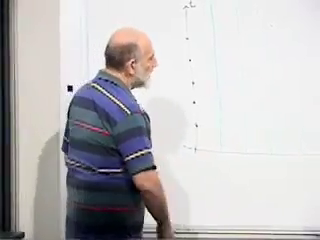
\includegraphics[width=0.62\textwidth]{lecture_01_figure_02.png}\caption{L’axe du temps dans le référentiel au repos et les premières lignes d’univers du réseau spatial.}\lectureframe{00:16:38}\end{figure}

On voit mieux cette même construction dans un schéma idéalisé :

\begin{figure}[H]\centering
\begin{tikzpicture}[scale=0.95]
\draw[->] (-1.2,0) -- (5.2,0) node[right] {$x$};
\draw[->] (0,-0.2) -- (0,4.8) node[above] {$t$};
\foreach \x in {-1,1,2,3,4}
  \draw[gray!65] (\x,0) -- (\x,4.4);
\foreach \y in {1,2,3,4}
  \draw[gray!65] (-1.0,\y) -- (4.4,\y);
\fill (0,0) circle (1.5pt);
\node[below left] at (0,0) {$0$};
\node[left] at (0,1) {$1$};
\node[left] at (0,2) {$2$};
\node[left] at (0,3) {$3$};
\node[below] at (1,0) {$1$};
\node[below] at (2,0) {$2$};
\node[below] at (3,0) {$3$};
\end{tikzpicture}\caption{Un réseau d’espace-temps au repos. Les droites verticales correspondent à une position constante ; les droites horizontales, à un instant constant.}\end{figure}

Le réseau est imaginaire et son espacement est arbitraire. On peut utiliser des mètres, des centimètres, des microns ou tout intervalle encore plus petit qui ait un sens physique. Il sert à attribuer des coordonnées précises à chaque événement.

L’expression « référentiel » prend maintenant un sens opérationnel. Elle ne désigne pas simplement un point de vue ou une personne qui regarde dans une direction donnée. C’est un dispositif de coordonnées étendu. Pour un événement donné, les règles locales indiquent où il s’est produit et l’horloge locale, quand. On peut alors comparer d’autres grandeurs physiques entre référentiels : la position et la vitesse d’une particule, son énergie, éventuellement la température d’un corps et, par la suite, sa quantité de mouvement et la force. La comparaison la plus simple porte sur \(x\) et \(t\) ; c’est par là que nous commencerons.

Plaçons maintenant un second réseau sur un train qui se déplace dans la direction positive de \(x\) à vitesse constante \(v\). Faisons coïncider les origines à \(t=0\). L’origine mobile suit alors la trajectoire
\begin{equation}
x=vt.
\end{equation}
Tout autre point fixe dans le train suit une ligne d’univers inclinée parallèle. Cette inclinaison exprime simplement le fait que le train change de position au fil du temps.

Supposons que le point arrière du train soit l’origine primée. À \(t=0\), elle coïncide avec l’origine de la gare. À un instant ultérieur \(t\), sa coordonnée dans le référentiel de la gare est \(vt\). Un événement voisin de coordonnée \(x\) ne se trouve donc qu’à une distance \(x-vt\) de l’origine du train. C’est pourquoi la transformation fait intervenir une soustraction, et non une règle algébrique arbitraire.

Notons \((x,t)\) les coordonnées d’un événement dans le référentiel de la gare et \((x',t')\) celles du même événement dans le référentiel du train. Pour Galilée et Newton, le temps reste universel :
\begin{equation}
t'=t.
\end{equation}
Pendant le temps \(t\), l’origine mobile avance de \(vt\) ; la distance entre cette origine et l’événement vaut donc
\begin{equation}
x'=x-vt.
\end{equation}
En réunissant ces relations,
\begin{align}
t'&=t, & x'&=x-vt.
\label{eq:galilean-forward}
\end{align}
On obtient la transformation inverse en isolant les coordonnées non primées :
\begin{align}
t&=t', & x&=x'+vt'.
\label{eq:galilean-inverse}
\end{align}

\begin{figure}[H]\centering
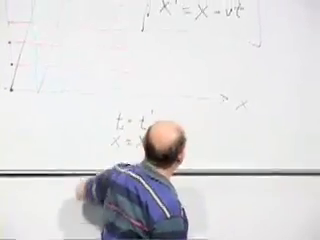
\includegraphics[width=0.72\textwidth]{lecture_01_figure_03.png}\caption{La transformation galiléenne, écrite à côté des deux réseaux d’espace-temps.}\lectureframe{00:21:57}\end{figure}

Le premier couple d’équations indique à l’observateur mobile comment convertir les coordonnées données par l’observateur au repos. Le couple inverse effectue la conversion en sens contraire. Cette conversion réciproque entre descriptions constitue le contenu mathématique de la relativité galiléenne.

Dans la formule spatiale inverse, la substitution \(t\to t'\) ne pose pas de problème uniquement parce que la théorie galiléenne a déjà posé \(t=t'\). Il est utile de relever cette hypothèse dès maintenant. Dans la théorie d’Einstein, les deux coordonnées temporelles différeront, et de telles substitutions ne seront plus automatiques.

\begin{classroomqa}\audiencequestion{Si l’on emporte une horloge puis qu’on la ramène, comment savoir que son mouvement ne l’a pas d’abord accélérée puis ralentie, masquant ainsi l’effet lorsqu’on compare les horloges ?\lecturetimestamp{00:23:09}}\lecturerresponse{Galilée n’aurait pas pu établir le caractère universel du temps avec la précision moderne ; il s’agissait d’une hypothèse physique. On peut la mettre à l’épreuve de nombreuses façons : transporter de bonnes horloges dans des directions opposées, refaire le trajet vers le nord--le sud autant que vers l’est--l’ouest, faire tourner une horloge autour de l’autre ou échanger des signaux horaires sans rapprocher les horloges. Aux vitesses ordinaires, tous ces tests concordent avec une très grande précision. Avec des horloges suffisamment précises ou des vitesses assez élevées, un faible écart apparaît. La défaillance du temps universel n’est pas un défaut de l’expérience : c’est un phénomène que la relativité restreinte doit expliquer.}\end{classroomqa}

\section{Invariants galiléens et loi de Newton}

Un invariant est une grandeur sur laquelle s’accordent tous les observateurs inertiels considérés. Les coordonnées elles-mêmes ne sont pas nécessairement invariantes. Il importe de savoir si les lois qu’on formule à partir d’elles conservent la même forme.

Le terme s’emploie comme nom et comme adjectif. Un nombre peut être un invariant, tout comme une équation peut être invariante sous une transformation. Distinguer les grandeurs invariantes des lois invariantes évite une confusion fréquente : la relativité ne prétend pas que tous les observateurs obtiennent les mêmes coordonnées pour tout. Elle affirme que la loi physique qui relie leurs mesures conserve la même forme.

Considérons deux événements simultanés situés aux positions \(x_1\) et \(x_2\). L’équation~\eqref{eq:galilean-forward} donne
\begin{align}
x_1'&=x_1-vt,\\
x_2'&=x_2-vt.
\end{align}
Leur séparation vaut donc
\begin{equation}
x_2'-x_1'=(x_2-vt)-(x_1-vt)=x_2-x_1.
\end{equation}
En physique galiléenne, la distance entre des événements qui se produisent au même instant est invariante, même si leurs positions respectives ne le sont pas.

\begin{classroomqa}\audiencequestion{Les deux occurrences de \(t\) dans cette soustraction représentent-elles vraiment le même instant ?\lecturetimestamp{00:28:16}}\lecturerresponse{Oui. Nous avons délibérément choisi deux événements \((x_1,t)\) et \((x_2,t)\) simultanés. Ils se trouvent sur une même droite horizontale de temps constant. Le terme commun \(vt\) s’annule donc. Si les événements se produisaient à des instants différents, ce raisonnement ne permettrait pas d’établir l’invariance de leur séparation spatiale.}\end{classroomqa}

Décrivons maintenant une particule par une trajectoire \(x(t)\). L’observateur du train lui attribue
\begin{equation}
x'(t)=x(t)-vt.
\end{equation}
En dérivant une fois, on obtient la règle usuelle d’addition des vitesses :
\begin{equation}
\frac{dx'}{dt}=\frac{dx}{dt}-v.
\end{equation}
La position et la vitesse dépendent du référentiel. Un observateur qui accompagne une flèche la voit se déplacer moins vite qu’un observateur placé au bord de la voie.

Dérivons une seconde fois. Comme la vitesse relative \(v\) est constante,
\begin{equation}
\frac{d^2x'}{dt^2}=\frac{d^2x}{dt^2}.
\end{equation}
L’accélération est invariante sous une transformation galiléenne. Cela suggère fortement pourquoi la loi de Newton s’exprime en fonction de l’accélération plutôt que de la position ou de la vitesse.

Il s’agit de l’accélération d’un objet observé, et non de celle de l’observateur dans le train. Les deux référentiels sont inertiels ; aucun n’accélère par rapport à l’autre. Dans chaque description, des objets peuvent accélérer vers la gauche ou vers la droite, et les deux observateurs s’accordent sur la valeur de cette accélération, même s’ils ne s’accordent pas sur la position ni sur la vitesse de l’objet.

Supposons que deux particules exercent l’une sur l’autre une force qui dépend uniquement de leur séparation mesurée au même instant. Cette séparation étant invariante, la force l’est aussi. Si la masse est également une propriété intrinsèque, indépendante du référentiel, chaque observateur inertiel peut écrire
\begin{equation}
F=ma
\end{equation}
exactement sous la même forme. La mécanique newtonienne est invariante sous les transformations galiléennes. Ce n’est pas seulement plausible : dans le domaine des vitesses ordinaires, elle est extraordinairement précise.

Le raisonnement s’applique aux forces centrales usuelles, comme la gravitation newtonienne ou l’électrostatique, dont l’intensité dépend de la distance. Tous les observateurs galiléens s’accordant sur cette distance à un instant donné, ils s’accordent aussi sur la force. Puisque la force et l’accélération sont fixées, la cohérence exige alors qu’ils s’accordent également sur la masse : un objet d’un kilogramme reste un objet d’un kilogramme lorsqu’il passe dans un train. Chaque symbole de \(F=ma\) s’inscrit dans la même structure invariante.

\section{La lumière ne suit pas la règle galiléenne}

L’électromagnétisme pose problème. Les équations de Maxwell prédisent des ondes qui se propagent dans le vide à une vitesse bien déterminée \(c\). Si les équations de Maxwell sont des lois de la nature et que celles-ci sont les mêmes dans chaque référentiel inertiel, alors tous les observateurs inertiels doivent mesurer la même valeur de \(c\).

La cinématique galiléenne prédit autre chose. Dans le référentiel au repos, une impulsion lumineuse qui se déplace vers la droite satisfait
\begin{equation}
x=ct.
\end{equation}
En appliquant la transformation spatiale, on obtient
\begin{equation}
x'=x-vt=(c-v)t.
\end{equation}
Comme \(t'=t\), l’observateur du train mesurerait la vitesse \(c-v\).

La contradiction peut se formuler sans ambiguïté. Si les équations de Maxwell conservent leur forme, elles prédisent \(c\) dans le référentiel primé. Si l’on conserve la transformation galiléenne, celle-ci prédit \(c-v\). Ces deux prédictions ne peuvent être exactes simultanément lorsque \(v\ne0\).

Ce résultat semble tout à fait naturel si la lumière se comporte comme une onde ordinaire dans un milieu. Un bateau porté par une vague mesure une vitesse de l’onde plus faible par rapport à lui. Un auditeur qui se déplace dans de l’air immobile mesure une vitesse du son décalée par rapport à son mouvement vis-à-vis de l’air. Les physiciens du XIXᵉ siècle ont donc envisagé un état de repos privilégié : le référentiel de l’éther, dans lequel les équations de Maxwell auraient leur forme la plus simple et où la lumière se propagerait à \(c\). Les expériences conçues pour détecter le mouvement par rapport à ce référentiel privilégié n’ont mis en évidence aucun effet correspondant.

Plusieurs dispositifs expérimentaux étaient possibles, mais tous visaient à comparer la propagation de la lumière pour des observateurs dont les mouvements différaient par leur état ou leur direction. Aucun n’a révélé le décalage galiléen attendu. Cet échec n’était pas une petite difficulté technique. Il imposait de choisir entre le principe de relativité, les équations de Maxwell et les conceptions héritées de l’espace et du temps.

Einstein a abordé le conflit plus directement. Jeune homme, il s’est imaginé poursuivant une onde lumineuse. S’il parvenait à la rattraper, son motif électromagnétique oscillant semblerait figé dans l’espace ; or les équations de Maxwell n’autorisent aucune onde lumineuse stationnaire de ce type. Il a choisi de considérer la théorie de Maxwell et le principe de relativité comme fondamentaux, puis de réexaminer les hypothèses dissimulées dans nos coordonnées.

La reconstruction repose sur deux postulats :
\begin{enumerate}\item Les lois de la physique ont la même forme dans tous les référentiels inertiels.
\item La lumière dans le vide se propage à la même vitesse \(c\) dans tous les référentiels inertiels.
\end{enumerate}

Le second postulat ne peut coexister avec la transformation galiléenne. Il faut modifier quelque chose de plus profond que la règle d’addition des vitesses. Einstein choisit, par souci d’économie, de conserver les deux postulats et de réexaminer l’équation galiléenne en apparence anodine \(t'=t\).

\section{Synchroniser des horloges éloignées}

On peut établir les distances spatiales à l’aide de règles, mais la synchronisation d’horloges éloignées nécessite une convention. Plaçons deux horloges à égale distance d’un observateur situé au milieu. Lorsque chaque horloge extrême indique l’instant convenu, faisons-lui émettre un éclair lumineux. Si les deux éclairs atteignent ensemble l’observateur, nous dirons que les horloges extrêmes sont synchronisées. Si l’un des éclairs arrive en premier, réglons l’horloge correspondante et recommençons la procédure.

Le terme \emph{milieu} est défini à l’aide des règles déjà disposées dans ce référentiel. Le test comporte donc deux éléments distincts : la même distance spatiale aux deux extrémités et le même instant d’arrivée des signaux. Il ne faut omettre ni l’un ni l’autre. En répétant la procédure sur tout le réseau, on établit les droites horizontales de temps constant que Newton avait simplement postulées.

Cette définition fait appel à la lumière parce que le postulat lui attribue la même vitesse dans tous les référentiels inertiels. Une fois que la procédure a été appliquée à toutes les paires voisines, l’ensemble du réseau est doté d’une famille d’horloges synchronisées.

Faisons maintenant traverser le premier réseau par un second réseau mobile. Dans son propre référentiel, le milieu du dispositif mobile reste à égale distance de ses deux extrémités. Par rapport au dispositif immobile, il se déplace toutefois en direction d’un éclair incident et s’éloigne de l’autre. Des éclairs émis simultanément selon les horloges du référentiel au repos n’arrivent donc pas ensemble au milieu du dispositif mobile. Comme l’observateur mobile applique la même règle du milieu et de la lumière, il ne peut pas considérer ces émissions comme simultanées. Chaque référentiel synchronise ses propres horloges de manière cohérente, mais les deux synchronisations ne concordent pas.

Il ne s’agit pas d’une illusion d’optique due au temps de parcours fini de la lumière. Chaque observateur sait que la lumière met du temps à arriver et en tient compte en utilisant la même vitesse \(c\). Le désaccord subsiste après cette correction, car les observateurs ne choisissent pas les mêmes événements éloignés comme paire simultanée. C’est la simultanéité elle-même qui est relative, et non pas seulement son apparence.

\begin{classroomqa}\audiencequestion{Pourrait-on éviter cette conclusion en synchronisant les horloges au moyen du son plutôt que de la lumière ?\lecturetimestamp{00:49:03}}\lecturerresponse{Le son peut servir de signal de synchronisation dans un référentiel où l’air est au repos, mais sa vitesse mesurée n’est pas la même dans tous les référentiels inertiels. Un train découvert qui roule dans de l’air immobile se déplace par rapport au milieu de propagation du son ; les signaux sonores vers l’avant et vers l’arrière ne s’y comportent donc pas symétriquement. Le postulat distingue la lumière : aucun milieu optique détectable ne définit un référentiel au repos qui privilégierait un observateur. Nous utilisons donc la lumière et en suivons les conséquences.}\end{classroomqa}

Le désaccord qualitatif est clair. Calculons maintenant précisément quels événements l’observateur mobile considère comme simultanés.

\section{Construction à l’aide de rayons lumineux}

Pour effectuer la construction, il est commode de choisir des unités telles que
\begin{equation}
c=1.
\end{equation}
Une unité de distance correspond alors à la distance parcourue par la lumière pendant une unité de temps : des secondes-lumière associées à des secondes, ou des années-lumière associées à des années. L’espace et le temps ont ainsi les mêmes unités, les vitesses sont sans dimension et les rayons lumineux apparaissent à \(45^\circ\). Un rayon dirigé vers la droite suit
\begin{equation}
x=t+d,
\end{equation}
tandis qu’un rayon dirigé vers la gauche suit
\begin{equation}
x=-t+d'.
\end{equation}
Les deux rayons qui passent par l’origine sont simplement \(x=t\) et \(x=-t\). Les trajectoires de genre temps, celles d’objets plus lents que la lumière, sont plus proches de l’axe vertical. Une trajectoire hypothétique supraluminique serait plus proche de l’axe horizontal.

L’angle du schéma n’a de sens qu’après ce choix d’unités. En mètres et en secondes, un rayon lumineux semblerait presque horizontal, puisqu’il parcourt environ \(3\times10^8\) mètres en une seconde. En choisissant la seconde-lumière comme unité de distance, on change l’échelle de l’axe horizontal et la géométrie causale devient visible.

Considérons trois lignes d’univers parallèles du réseau mobile,
\begin{equation}
x=vt,\qquad x=vt+L,\qquad x=vt+2L.
\label{eq:moving-worldlines}
\end{equation}
La ligne d’univers centrale est celle de l’observateur qui teste la simultanéité entre les deux points extrêmes. Les trois points se déplacent uniformément et conservent leur disposition relative dans le référentiel primé.

\begin{figure}[H]\centering
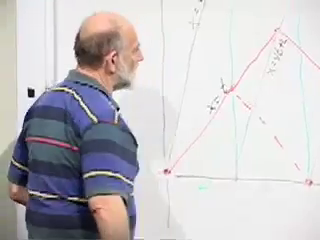
\includegraphics[width=0.72\textwidth]{lecture_01_figure_04.png}\caption{Le rayon lumineux vers l’avant \(x=t\) rencontre la ligne d’univers centrale du référentiel mobile.}\lectureframe{01:02:33}\end{figure}

On peut représenter la géométrie complète sans l’obstruction d’une personne devant le tableau :

\begin{figure}[H]\centering
\begin{tikzpicture}[scale=0.95]
\draw[->] (-0.5,0) -- (6.5,0) node[right] {$x$};
\draw[->] (0,-0.2) -- (0,4.3) node[above] {$t$};
\draw[blue] (0,0) -- (1.4,4.0);
\draw[blue] (2.0,0) -- (3.4,4.0);
\draw[blue] (4.0,0) -- (5.4,4.0);
\draw[red] (0,0) -- (3.08,3.08);
\draw[red] (3.08,3.08) -- (4.56,1.60);
\draw[red,dashed] (2.0,0) -- (4.56,1.60);
\fill (0,0) circle (1.5pt);
\fill (2.0,0) circle (1.5pt);
\fill (4.0,0) circle (1.5pt);
\fill (3.08,3.08) circle (1.5pt);
\fill (4.56,1.60) circle (1.5pt);
\node[left] at (0.55,1.55) {$x=vt$};
\node[left] at (2.45,1.9) {$x=vt+L$};
\node[right] at (4.72,1.9) {$x=vt+2L$};
\node[left] at (1.88,2.28) {$x=t$};
\node[above right] at (3.08,3.08) {$A$};
\end{tikzpicture}\caption{Les signaux lumineux déterminent la ligne de simultanéité du référentiel mobile.}\end{figure}

Émettons un rayon lumineux vers la droite depuis l’origine. Notons \(A\) son intersection avec la ligne d’univers centrale. Les deux équations en \(A\) sont
\begin{align}
x&=t,\\
x&=vt+L.
\end{align}
En substituant, on obtient
\begin{equation}
t=vt+L,
\end{equation}
d’où
\begin{equation}
t_A=x_A=\frac{L}{1-v}.
\label{eq:point-a}
\end{equation}

À partir de \(A\), suivons en arrière un rayon lumineux dirigé vers la gauche jusqu’à la ligne d’univers mobile la plus à droite. Son équation est de la forme
\begin{equation}
x+t=b.
\end{equation}
Comme il passe par \(A\), l’équation~\eqref{eq:point-a} détermine la constante :
\begin{equation}
b=x_A+t_A=\frac{2L}{1-v}.
\end{equation}
Le rayon suivi vers l’arrière satisfait donc
\begin{equation}
x+t=\frac{2L}{1-v}.
\label{eq:backward-ray}
\end{equation}

Son intersection avec la ligne d’univers la plus à droite est donnée par
\begin{align}
x+t&=\frac{2L}{1-v},\\
x&=vt+2L.
\end{align}
Éliminons \(x\) :
\begin{align}
(1+v)t
  &=2L\left(\frac{1}{1-v}-1\right)\\
  &=\frac{2Lv}{1-v},
\end{align}
d’où
\begin{equation}
t=\frac{2Lv}{1-v^2}.
\end{equation}
En substituant dans \(x=vt+2L\), on obtient
\begin{equation}
x=\frac{2L}{1-v^2}.
\end{equation}
Les coordonnées elles-mêmes importent moins que leur rapport :
\begin{equation}
\frac{t}{x}=v.
\end{equation}
Ainsi, tout événement simultané avec l’origine selon les horloges mobiles se trouve sur
\begin{equation}
t=vx,
\label{eq:simultaneity-c-one}
\end{equation}
tandis que l’origine mobile suit
\begin{equation}
x=vt.
\label{eq:moving-time-axis}
\end{equation}
Les deux axes sont inclinés symétriquement autour du rayon lumineux à \(45^\circ\).

Tous les points de \(x=vt\) ont la même position primée, \(x'=0\), tandis que leur temps primé varie. Tous les points de \(t=vx\) ont le même temps primé, \(t'=0\), tandis que leur position primée varie. L’une de ces droites est donc l’axe du temps primé et l’autre, l’axe de l’espace primé. Cette longue construction à l’aide de signaux était nécessaire pour déterminer la seconde droite ; on ne pouvait pas la déduire de la seule ligne d’univers mobile.

Pour rétablir les unités usuelles dans l’équation~\eqref{eq:simultaneity-c-one}, il faut écrire
\begin{equation}
t=\frac{v}{c^2}x.
\label{eq:simultaneity-dimensional}
\end{equation}
Le facteur \(c^2\) explique pourquoi la représentation newtonienne fonctionne si bien dans la vie quotidienne. Pour des vitesses très faibles devant \(c\), la pente de la ligne de simultanéité mobile est extrêmement petite.

\begin{figure}[H]\centering
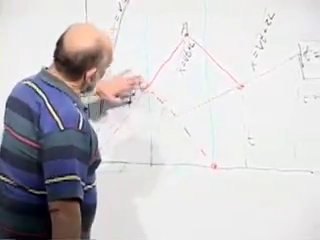
\includegraphics[width=0.72\textwidth]{lecture_01_figure_05.png}\caption{Pour \(c=1\), les axes primés du temps et de la simultanéité sont symétriques par rapport au rayon lumineux.}\lectureframe{01:15:40}\end{figure}

\begin{figure}[H]\centering
\begin{tikzpicture}[scale=1.0]
\draw[->] (-2.2,0) -- (5.2,0) node[right] {$x$};
\draw[->] (0,-0.2) -- (0,4.9) node[above] {$t$};
\draw[red] (0,0) -- (3.9,3.9);
\draw[red] (0,0) -- (-1.8,1.8);
\draw[blue] (0,0) -- (1.8,4.5);
\draw[blue,dashed] (0,0) -- (4.5,1.8);
\node[right] at (3.9,3.9) {$x=t$};
\node[left] at (-1.8,1.8) {$x=-t$};
\node[above] at (1.8,4.5) {$x'=0$};
\node[right] at (4.5,1.8) {$t'=0$};
\end{tikzpicture}\caption{Les axes primés et les rayons lumineux invariants en unités où \(c=1\).}\end{figure}

\section{Dérivation de la transformation de Lorentz}

La géométrie fixe les lieux où chaque coordonnée primée s’annule. Sur l’axe du temps mobile \(x=vt\), il faut que \(x'=0\). Sur l’axe de simultanéité mobile \(t=vx\), il faut que \(t'=0\). Les relations linéaires les plus générales ayant ces ensembles de zéros peuvent s’écrire
\begin{align}
x'&=\frac{x-vt}{F(v)},\\
t'&=\frac{t-vx}{G(v)}.
\label{eq:fg-ansatz}
\end{align}
Les facteurs \(F\) et \(G\) permettent aux échelles des coordonnées primées de différer des échelles galiléennes, bien que les axes aient déjà été localisés. La linéarité découle de l’homogénéité de l’espace et du temps : une translation de l’expérience ne peut modifier la loi de transformation.\editorialnote{Cet argument succinct sur la linéarité explicite une hypothèse utilisée implicitement dans la dérivation au tableau.}

À ce stade, la géométrie nous a appris beaucoup, mais pas tout. Les numérateurs déterminent l’inclinaison des axes. Ils ne déterminent pas l’espacement des unités le long de ces axes. C’est précisément cette information d’échelle restante que représentent \(F(v)\) et \(G(v)\).

Imposons maintenant l’invariance de la vitesse de la lumière. Un rayon dirigé vers la droite, qui satisfait \(x=t\), doit aussi satisfaire \(x'=t'\). Le long de ce rayon,
\begin{align}
x'&=\frac{(1-v)t}{F(v)},\\
t'&=\frac{(1-v)t}{G(v)}.
\end{align}
L’égalité doit tenir en chaque point du rayon, ce qui impose
\begin{equation}
F(v)=G(v).
\end{equation}
Nous pouvons donc écrire
\begin{align}
x'&=\frac{x-vt}{F(v)},\\
t'&=\frac{t-vx}{F(v)}.
\label{eq:common-f}
\end{align}

Cette étape fait intervenir, pour la première fois dans le calcul, une exigence proprement einsteinienne. Une même droite géométrique représente un rayon lumineux pour les deux observateurs ; les deux coordonnées primées doivent donc augmenter à la même vitesse le long de cette droite lorsque \(c=1\). Des facteurs différents dans les deux équations donneraient une vitesse primée différente de l’unité.

Il reste une fonction inconnue. Multiplions l’équation~\eqref{eq:common-f} par \(F(v)\) :
\begin{align}
F(v)x'&=x-vt,\\
F(v)t'&=t-vx.
\end{align}
En multipliant la seconde équation par \(v\), puis en l’ajoutant à la première, on élimine \(t\) et l’on obtient
\begin{equation}
(1-v^2)x=F(v)(x'+vt').
\end{equation}
De même,
\begin{equation}
(1-v^2)t=F(v)(t'+vx').
\end{equation}
La transformation inverse est donc
\begin{align}
x&=\frac{F(v)}{1-v^2}(x'+vt'),\\
t&=\frac{F(v)}{1-v^2}(t'+vx').
\end{align}

Le principe de relativité rend les deux référentiels réciproques. Si la gare voit le train se déplacer à \(+v\), le train voit la gare se déplacer à \(-v\). Les équations inverses doivent donc avoir la même forme que les équations directes, avec le signe de \(v\) inversé. Leurs facteurs de proportionnalité doivent satisfaire
\begin{equation}
\frac{F(v)}{1-v^2}=\frac{1}{F(v)}.
\end{equation}
D’où
\begin{equation}
F(v)^2=1-v^2,
\end{equation}
et la continuité avec la transformation identité pour \(v=0\) sélectionne la racine positive :
\begin{equation}
F(v)=\sqrt{1-v^2}.
\end{equation}

Aucun rayon lumineux particulier n’a servi à ajuster le résultat. Celui-ci découle des axes fixés par la synchronisation, de l’universalité de la vitesse de la lumière et de l’exigence qu’aucun des deux référentiels inertiels ne soit privilégié par rapport à l’autre.

La transformation de Lorentz en unités où \(c=1\) s’écrit
\begin{align}
x'&=\frac{x-vt}{\sqrt{1-v^2}},\\
t'&=\frac{t-vx}{\sqrt{1-v^2}}.
\label{eq:lorentz-c-one}
\end{align}
Sa transformation inverse est
\begin{align}
x&=\frac{x'+vt'}{\sqrt{1-v^2}},\\
t&=\frac{t'+vx'}{\sqrt{1-v^2}}.
\end{align}

\begin{figure}[H]\centering
\includegraphics[width=0.76\textwidth]{lecture_01_figure_06.png}\caption{La transformation de Lorentz complète en unités où \(c=1\), écrite au tableau.}\lectureframe{01:32:38}\end{figure}

La nouveauté essentielle apparaît déjà dans l’équation du temps. Le temps n’est pas simplement transmis sans changement d’un référentiel à l’autre. La coordonnée temporelle primée combine le temps et la position non primés. Par conséquent, \(t=\text{constant}\) et \(t'=\text{constant}\) décrivent des ensembles différents d’événements.

Le terme de mélange n’est pas une correction facultative ajoutée après coup. Sans lui, la droite \(t'=0\) resterait horizontale, la simultanéité à distance demeurerait universelle et la transformation ne pourrait pas préserver la vitesse de la lumière.

\section{Rétablir la vitesse de la lumière et vérifier le résultat}

Lorsque \(c\ne1\), la cohérence dimensionnelle rétablit les facteurs manquants. Le rapport \(v^2/c^2\) est sans dimension, tandis que \((v/c^2)x\) a les dimensions d’un temps. On a donc
\begin{align}
x'&=\frac{x-vt}{\sqrt{1-v^2/c^2}},\\
t'&=\frac{t-(v/c^2)x}{\sqrt{1-v^2/c^2}}.
\label{eq:lorentz-dimensional}
\end{align}
On obtient la transformation inverse en inversant le signe de \(v\) :
\begin{align}
x&=\frac{x'+vt'}{\sqrt{1-v^2/c^2}},\\
t&=\frac{t'+(v/c^2)x'}{\sqrt{1-v^2/c^2}}.
\end{align}
En introduisant
\begin{equation}
\gamma=\frac{1}{\sqrt{1-v^2/c^2}}
\end{equation}
on obtiendrait la forme compacte usuelle, mais l’écriture avec le dénominateur permet de suivre la dérivation.

Numériquement, \(c\simeq3\times10^8\,\mathrm{m/s}\), donc \(c^2\simeq9\times10^{16}\,\mathrm{m^2/s^2}\). Le grand dénominateur rend imperceptibles, dans la plupart des expériences mécaniques, l’inclinaison de la simultanéité et le facteur \(v^2/c^2\). Leur petitesse explique le succès de Galilée ; elle ne rétablit pas le temps absolu.

\begin{figure}[H]\centering
\includegraphics[width=0.76\textwidth]{lecture_01_figure_07.png}\caption{La transformation de Lorentz après rétablissement des facteurs de \(c\).}\lectureframe{01:35:58}\end{figure}

Deux vérifications s’imposent immédiatement. Commençons par \(v\ll c\). Alors, \(v^2/c^2\) est négligeable et, pour des distances ordinaires, le terme de relativité de la simultanéité \(vx/c^2\) l’est aussi. L’équation~\eqref{eq:lorentz-dimensional} se réduit à
\begin{equation}
t'\approx t,\qquad x'\approx x-vt.
\end{equation}
On retrouve la relativité galiléenne comme approximation aux faibles vitesses.

Deuxièmement, considérons un rayon lumineux. Une fois \(c\) rétabli, un rayon se propageant vers la droite obéit à \(x=ct\), et non à \(x=t\). La substitution donne
\begin{align}
x'&=\frac{(c-v)t}{\sqrt{1-v^2/c^2}},\\
t'&=\frac{(1-v/c)t}{\sqrt{1-v^2/c^2}}.
\end{align}
Puisque \(c-v=c(1-v/c)\),
\begin{equation}
x'=ct'.
\end{equation}
L’observateur primé mesure la même vitesse \(c\). Pour un rayon se propageant vers la gauche, la substitution de \(x=-ct\) donne de même
\begin{equation}
x'=-ct'.
\end{equation}
La transformation décrit correctement la lumière se propageant dans les deux directions.

La distinction entre \(x=t\) et \(x=ct\) constitue une vérification dimensionnelle instructive. La première expression n’est correcte que dans un système d’unités où \(c=1\). Rétablir les unités usuelles dans la transformation tout en laissant l’équation du rayon en unités naturelles reviendrait à mélanger deux conventions et conduirait à un résultat erroné. La cohérence dimensionnelle permet de repérer immédiatement l’erreur.

\section{Le critère du point milieu}

\begin{classroomqa}
\audiencequestion{Un observateur reçoit deux éclairs lumineux au même instant, mais il ne se trouve pas à mi-distance de leurs sources. Peut-il en conclure que les éclairs ont été émis simultanément ?
\lecturetimestamp{01:42:55}}
\lecturerresponse{Non. Des temps d’arrivée égaux impliquent des temps d’émission égaux uniquement pour l’observateur situé à mi-distance spatiale des deux sources dans le référentiel considéré. Un récepteur plus proche de l’une des sources peut recevoir les deux éclairs en même temps alors que l’éclair le plus éloigné a été émis plus tôt. Dans la construction en mouvement, la ligne d’univers du point milieu \(x=vt+L\) est donc essentielle. On suit le rayon lumineux dirigé vers l’avant \(x=t\) jusqu’à ce qu’il rencontre ce point milieu, puis on trace un rayon lumineux vers l’arrière jusqu’à \(x=vt+2L\). Cet événement à la seconde extrémité, et non un événement quelconque d’arrivée simultanée ailleurs, est simultané à l’origine selon le référentiel en mouvement.}
\end{classroomqa}

Nous sommes parvenus à la transformation complète des coordonnées, mais pas encore à ses conséquences les plus connues. Nous examinerons ensuite la contraction des longueurs, la dilatation du temps et le temps propre, puis la quantité de mouvement et l’énergie relativistes. Les bases sont déjà posées : chaque référentiel inertiel ne peut appliquer les mêmes lois et mesurer la même vitesse de la lumière que parce que l’espace et le temps se mélangent, et parce que la simultanéité à distance est propre à un référentiel, et non au monde en soi.

\chapter{Équations de Maxwell, covariance et ondes électromagnétiques}

\lectureoverview{Les champs électrique et magnétique agissent sur la matière chargée par l’intermédiaire de la force de Lorentz, mais la matière doit aussi créer et réorganiser les champs. Nous formulerons cette réciprocité de l’électromagnétisme, montrerons que les équations de Maxwell sont covariantes de Lorentz, en dériverons les solutions ondulatoires, puis réintroduirons la charge et le courant sous une forme qui rend manifeste la conservation locale. Dans tout ce cours, nous utilisons des unités telles que \(c=1\).}

\section{L’autre aspect de l’électromagnétisme}

Commençons par la partie du sujet déjà étudiée. Si une particule de charge \(q\) se déplace à la vitesse \(\mathbf v\) dans des champs électrique et magnétique, la force est
\begin{equation}
\mathbf F=q\bigl(\mathbf E+\mathbf v\times\mathbf B\bigr).
\label{eq:lorentz-force-three}
\end{equation}
Le facteur \(q\) est indispensable. Une particule non chargée ne subit pas la force électromagnétique. Le champ électrique contribue même lorsque la particule est momentanément au repos, tandis que la contribution magnétique dépend de son mouvement.

L’équation~\eqref{eq:lorentz-force-three} nous indique l’effet de champs prescrits sur la matière. Elle ne nous dit pas ce qui détermine les champs. Qu’est-ce qui produit un champ électrique autour d’un objet, un champ magnétique autour d’un autre, ou une onde qui se propage dans le vide ? Les équations qui répondent à ces questions sont les équations de Maxwell.

\begin{figure}[H]
\centering
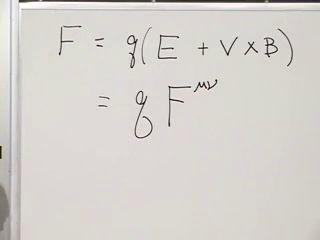
\includegraphics[width=0.62\textwidth]{lecture_58_figure_02.png}
\caption{La force de Lorentz en trois dimensions et le début de sa reformulation tensorielle.}
\lectureframe{00:05:49}
\end{figure}

La forme relativiste de la loi de force annonce les notations dont nous aurons besoin :
\begin{equation}
f^\mu=qF^\mu{}_{\nu}u^\nu.
\label{eq:lorentz-force-four}
\end{equation}
Ici, \(u^\nu\) est la quadrivitesse, \(f^\mu\) la quadri-force, et \(F^{\mu\nu}\) un tenseur antisymétrique construit à partir de \(\mathbf E\) et \(\mathbf B\). Au tableau, on n’en écrit d’abord que le début schématique ; la contraction avec \(u^\nu\) fournit le vecteur manquant et laisse un indice de force libre.

Il y a une raison physique pour laquelle la matière doit agir en retour sur le champ. Une onde électromagnétique peut frapper une charge, l’accélérer et lui transférer de l’énergie. Si le champ pouvait agir sur la charge sans que celle-ci puisse jamais agir sur le champ, il n’y aurait aucune source à laquelle retirer cette énergie. L’action et la réaction ne suffisent pas tout à fait à expliquer cela, mais la conservation de l’énergie rend inévitable ce couplage réciproque.

\section{Une source variable émet une perturbation}

Une charge ponctuelle produit un champ électrique dirigé vers l’extérieur ou vers l’intérieur à partir de sa position. Un courant dans un fil--un flux de particules chargées--produit un champ magnétique qui circule autour du fil. Ces images familières de situations statiques montrent déjà deux configurations géométriques différentes : le flux électrique émane des charges, tandis que les lignes de champ magnétique s’enroulent autour du courant.

Déplaçons maintenant brusquement la charge ponctuelle. Près de sa nouvelle position, le champ électrique doit commencer à se réorganiser, mais un observateur éloigné ne peut pas apprendre instantanément que la charge s’est déplacée. Au loin, l’ancien champ persiste jusqu’à l’arrivée du signal. Entre les régions proche et lointaine se trouve un front mobile où le champ est en train de changer. Cette réorganisation qui se propage est une perturbation électromagnétique.

Si la charge est animée d’un mouvement de va-et-vient, des réorganisations successives se suivent et forment une onde électromagnétique. C’est le fonctionnement élémentaire d’une antenne : un courant électrique oscillant émet une perturbation du champ vers l’extérieur. Inverser le sens du courant dans un fil conduit au même raisonnement pour le champ magnétique. Le sens de circulation de \(\mathbf B\) doit s’inverser, mais cette inversion se propage au lieu d’apparaître partout à la fois.

Cette image causale fixe deux objectifs aux équations de Maxwell. Elles doivent décrire comment la charge et le courant sont à l’origine des champs, et permettre aux variations de ces champs de se propager à une vitesse qui ne dépasse pas celle de la lumière. Le second objectif met aussi la relativité à l’épreuve. Si les équations de Maxwell ont la même forme dans tous les référentiels inertiels et impliquent une vitesse d’onde bien déterminée, alors elles doivent conduire chaque référentiel inertiel à déduire la même vitesse.

\section{Rappel sur l’équation d’onde relativiste}

Avant de passer aux champs vectoriels, considérons un champ scalaire \(\phi(\mathbf x,t)\), qui prend une valeur numérique en chaque point de l’espace-temps. Une équation du premier ordre,
\begin{equation}
\partial_\mu\phi=0
\end{equation}
signifierait que toutes les dérivées spatio-temporelles s’annulent. Le champ serait constant et ne pourrait donc pas porter d’onde. Une équation d’onde relativiste non triviale fait intervenir deux dérivées :
\begin{equation}
\partial_\mu\partial^\mu\phi=0.
\end{equation}
Avec la convention de signe utilisée ici,
\begin{equation}
\left(\partial_t^2-\partial_x^2-\partial_y^2-\partial_z^2\right)\phi=0,
\label{eq:scalar-wave-four}
\end{equation}
ou, sous une forme plus compacte,
\begin{equation}
\left(\partial_t^2-\nabla^2\right)\phi=0.
\end{equation}
Le choix \(c=1\) permet d’exprimer le temps et les distances dans des unités compatibles. Si l’on rétablit les unités usuelles, le facteur \(1/c^2\) apparaît devant la dérivée temporelle seconde.

Pour une onde qui se propage le long de l’axe \(z\), le champ dépend de \(z\) et de \(t\), mais ni de \(x\) ni de \(y\). L’équation~\eqref{eq:scalar-wave-four} se réduit à
\begin{equation}
\left(\partial_t^2-\partial_z^2\right)\phi=0.
\label{eq:scalar-wave-one}
\end{equation}

\begin{figure}[H]
\centering
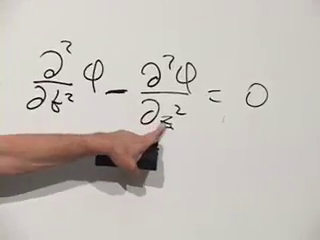
\includegraphics[width=0.56\textwidth]{lecture_58_figure_04.png}
\caption{L’équation d’onde scalaire à une dimension, modèle des ondes électromagnétiques.}
\lectureframe{00:47:03}
\end{figure}

La forme générale d’une onde progressive est
\begin{equation}
\phi(z,t)=f(z-t)+g(z+t).
\end{equation}
Le profil \(f(z-t)\) se propage dans le sens des \(z\) croissants, car un point de phase constante vérifie \(z-t=\text{constant}\). Le profil \(g(z+t)\) se propage dans le sens opposé. Rien n’impose que l’un ou l’autre profil soit sinusoïdal ; toute forme suffisamment régulière se translate sans se déformer.

Les sinusoïdes sont néanmoins commodes :
\begin{equation}
\phi(z,t)=A\cos\!\bigl(k(z-t)\bigr).
\end{equation}
Le nombre d’onde \(k\) détermine la longueur d’onde :
\begin{equation}
\lambda=\frac{2\pi}{k}.
\end{equation}
Une grande valeur de \(k\) produit des oscillations spatiales rapides et une courte longueur d’onde ; une petite valeur de \(k\) produit une longue longueur d’onde. Ces mêmes profils deviendront bientôt des composantes de \(\mathbf E\) et de \(\mathbf B\).

\section{Les outils de calcul vectoriel nécessaires aux équations de Maxwell}

Les équations de Maxwell font intervenir des produits scalaires, des produits vectoriels, la divergence et le rotationnel. Il est utile de reprendre une fois ces notations, car les calculs en composantes qui suivent reposent précisément sur ces opérations.

Pour les vecteurs usuels \(\mathbf a\) et \(\mathbf b\), le produit scalaire est le scalaire
\begin{equation}
\mathbf a\cdot\mathbf b
=a_xb_x+a_yb_y+a_zb_z.
\end{equation}
Le produit vectoriel est un autre vecteur :
\begin{align}
(\mathbf a\times\mathbf b)_x&=a_yb_z-a_zb_y,\\
(\mathbf a\times\mathbf b)_y&=a_zb_x-a_xb_z,\\
(\mathbf a\times\mathbf b)_z&=a_xb_y-a_yb_x.
\end{align}
Les autres composantes s’obtiennent en suivant l’ordre cyclique \(x\to y\to z\to x\).

Introduisons l’opérateur différentiel
\begin{equation}
\boldsymbol\nabla=
\left(\partial_x,\partial_y,\partial_z\right).
\end{equation}
Ses composantes sont des opérateurs, et non des nombres ordinaires, mais on peut tout de même utiliser les schémas du produit scalaire et du produit vectoriel. Pour un champ vectoriel \(\mathbf A\),
\begin{equation}
\boldsymbol\nabla\cdot\mathbf A
=\partial_xA_x+\partial_yA_y+\partial_zA_z
\label{eq:divergence}
\end{equation}
est la divergence, tandis que
\begin{align}
(\boldsymbol\nabla\times\mathbf A)_x
 &=\partial_yA_z-\partial_zA_y,\\
(\boldsymbol\nabla\times\mathbf A)_y
 &=\partial_zA_x-\partial_xA_z,\\
(\boldsymbol\nabla\times\mathbf A)_z
 &=\partial_xA_y-\partial_yA_x
\label{eq:curl}
\end{align}
en donne les composantes du rotationnel.

La géométrie compte autant que les formules. La divergence d’un champ vectoriel est positive là où le champ semble s’écouler vers l’extérieur à partir d’une source. Son rotationnel est non nul là où le champ circule. Le champ électrique radial d’une charge ponctuelle illustre la divergence ; le champ magnétique qui s’enroule autour d’un fil parcouru par un courant illustre le rotationnel. Un champ vectoriel uniforme n’a ni l’un ni l’autre.

\section{Les équations de Maxwell dans le vide}

En l’absence de charge et de courant, les équations de Maxwell sont
\begin{align}
\boldsymbol\nabla\times\mathbf E&=-\partial_t\mathbf B,
\label{eq:faraday-vac}\\
\boldsymbol\nabla\cdot\mathbf B&=0,
\label{eq:gauss-b-vac}\\
\boldsymbol\nabla\times\mathbf B&=\partial_t\mathbf E,
\label{eq:ampere-vac}\\
\boldsymbol\nabla\cdot\mathbf E&=0.
\label{eq:gauss-e-vac}
\end{align}
Les deux équations faisant intervenir le rotationnel échangent presque \(\mathbf E\) et \(\mathbf B\), mais un signe moins essentiel les distingue. Les deux équations de divergence indiquent qu’aucun des deux champs n’a de source dans la région de vide considérée. La divergence du champ magnétique reste nulle même lorsque l’on réintroduit les sources électriques ; l’électromagnétisme usuel ne comporte pas de charge magnétique.

\begin{figure}[H]
\centering
\includegraphics[width=0.76\textwidth]{lecture_58_figure_06.png}
\caption{Les quatre équations de Maxwell dans le vide, disposées de manière à faire ressortir la quasi-symétrie entre les champs électrique et magnétique.}
\lectureframe{00:27:30}
\end{figure}

La densité de charge \(\rho\) remplacera finalement le zéro à droite de l’équation~\eqref{eq:gauss-e-vac}, et la densité de courant \(\mathbf J\) apparaîtra dans l’équation~\eqref{eq:ampere-vac}. Nous mettons provisoirement ces termes de côté. Les équations sans sources font apparaître la structure des transformations et le mécanisme de propagation des ondes avec le moins de termes possible.

Elles précisent aussi l’énigme d’Einstein. Un observateur galiléen qui suit une onde s’attendrait à soustraire des vitesses et à mesurer une vitesse d’onde plus faible. Pourtant, si les mêmes équations de Maxwell valent dans tous les référentiels inertiels, chacun déduit une vitesse d’onde égale à l’unité. La solution ne consiste pas à modifier l’équation d’onde d’un référentiel à l’autre. Elle consiste à utiliser la transformation de Lorentz et à exprimer les équations de Maxwell au moyen d’objets dont les lois de transformation sont déjà connues.

\section{Les champs électrique et magnétique réunis en un seul tenseur}

Les champs électrique et magnétique se réunissent dans le tenseur de champ antisymétrique
\begin{equation}
F^{\mu\nu}=
\begin{pmatrix}
0   & -E_x & -E_y & -E_z\\
E_x & 0    & -B_z & B_y\\
E_y & B_z  & 0    & -B_x\\
E_z & -B_y & B_x  & 0
\end{pmatrix},
\label{eq:l0203-field-tensor}
\end{equation}
où l’ordre des lignes et des colonnes est \(t,x,y,z\). L’antisymétrie,
\begin{equation}
F^{\mu\nu}=-F^{\nu\mu},
\end{equation}
impose l’annulation des éléments diagonaux et détermine la moitié inférieure de la matrice à partir de la moitié supérieure. Les composantes temps-espace contiennent \(\mathbf E\) ; les composantes purement spatiales contiennent \(\mathbf B\).

\begin{figure}[H]
\centering
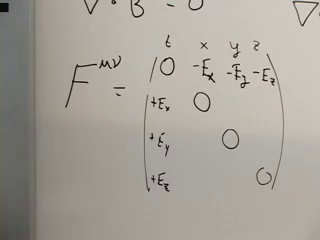
\includegraphics[width=0.58\textwidth]{lecture_58_figure_03.png}
\caption{Le tenseur électromagnétique complet, avec ses composantes électrique et magnétique.}
\lectureframe{00:32:05}
\end{figure}

L’importance de \(F^{\mu\nu}\) ne tient pas seulement au fait que six composantes du champ tiennent dans une même matrice. Sous une transformation de Lorentz, il se transforme comme un tenseur de rang deux. Les champs électrique et magnétique mesurés par des observateurs différents se mélangent donc exactement comme il le faut pour que l’ensemble se transforme de manière cohérente.

Il existe un second tenseur antisymétrique, le tenseur dual du champ \(\widetilde F^{\mu\nu}\). Avec la convention adoptée ici, on l’obtient à partir de l’équation~\eqref{eq:l0203-field-tensor} en effectuant le remplacement
\begin{equation}
\mathbf E\longmapsto-\mathbf B,
\qquad
\mathbf B\longmapsto\mathbf E.
\label{eq:dual-replacement}
\end{equation}
On obtient ainsi
\begin{equation}
\widetilde F^{\mu\nu}=
\begin{pmatrix}
0    & B_x  & B_y  & B_z\\
-B_x & 0    & -E_z & E_y\\
-B_y & E_z  & 0    & -E_x\\
-B_z & -E_y & E_x  & 0
\end{pmatrix}.
\label{eq:dual-tensor}
\end{equation}
Le signe dans l’équation~\eqref{eq:dual-replacement} est important. Pendant le cours, l’échange est d’abord énoncé verbalement ; on repère ensuite l’incohérence de signe et on la corrige avant de compléter la matrice.

\begin{figure}[H]
\centering
\includegraphics[width=0.58\textwidth]{lecture_58_figure_07.png}
\caption{Construction du tenseur dual par échange des composantes électrique et magnétique, avec le signe nécessaire.}
\lectureframe{00:35:45}
\end{figure}

\section{Les équations covariantes dans le vide}

Chaque équation de Maxwell contient une dérivée. La contraction d’un indice de dérivée avec un tenseur de rang deux laisse un indice libre ; les formes covariantes naturelles sont donc
\begin{align}
\partial_\mu F^{\mu\nu}&=0,
\label{eq:maxwell-covariant-vac}\\
\partial_\mu\widetilde F^{\mu\nu}&=0.
\label{eq:maxwell-dual-vac}
\end{align}
Pour chaque valeur fixée de \(\nu\), l’équation~\eqref{eq:maxwell-covariant-vac} constitue une équation. Comme \(\nu\) peut prendre les valeurs \(t,x,y,z\), elle regroupe quatre équations scalaires. L’équation~\eqref{eq:maxwell-dual-vac} en regroupe quatre autres. Cela correspond aux deux équations vectorielles faisant intervenir le rotationnel et aux deux équations scalaires de divergence de la liste initiale.

Une notation compacte n’est utile que si elle reproduit les équations familières. Prenons \(\nu=z\) :
\begin{align}
\partial_\mu F^{\mu z}
&=\partial_tF^{tz}
  +\partial_xF^{xz}
  +\partial_yF^{yz}
  +\partial_zF^{zz}\\
&=-\partial_tE_z+\partial_xB_y-\partial_yB_x\\
&=-\partial_tE_z+
  \bigl(\boldsymbol\nabla\times\mathbf B\bigr)_z.
\end{align}
Le terme \(F^{zz}\) s’annule par antisymétrie. En égalant le résultat à zéro, on obtient la composante \(z\) de
\begin{equation}
\boldsymbol\nabla\times\mathbf B=\partial_t\mathbf E.
\end{equation}
Les composantes \(x\) et \(y\) s’obtiennent par permutation cyclique des indices.

\begin{figure}[H]
\centering
\includegraphics[width=0.76\textwidth]{lecture_58_figure_08.png}
\caption{Développement en composantes de l’équation de champ covariante ; l’élément diagonal du tenseur s’annule et les termes restants reconstituent les équations de Maxwell.}
\lectureframe{00:43:30}
\end{figure}

Considérons maintenant la composante temporelle :
\begin{align}
\partial_\mu F^{\mu t}
&=\partial_tF^{tt}
  +\partial_xF^{xt}
  +\partial_yF^{yt}
  +\partial_zF^{zt}\\
&=\partial_xE_x+\partial_yE_y+\partial_zE_z\\
&=\boldsymbol\nabla\cdot\mathbf E.
\end{align}
On obtient donc l’équation~\eqref{eq:gauss-e-vac}. Les mêmes vérifications appliquées au tenseur dual donnent
\(\boldsymbol\nabla\cdot\mathbf B=0\) ainsi que
\(\boldsymbol\nabla\times\mathbf E=-\partial_t\mathbf B\).

Les équations compactes sont maintenant établies, et non simplement conjecturées. La structure de leurs indices libres en fait des équations à quatre composantes ; une transformation de Lorentz modifie donc leurs composantes, mais pas leur forme. C’est en ce sens précis que les équations de Maxwell dans le vide sont les mêmes dans tous les référentiels inertiels.

\section{Des équations du premier ordre aux ondes}

Les équations de Maxwell ne contiennent que des dérivées du premier ordre, tandis qu’une équation d’onde fait intervenir des dérivées secondes. Cette différence apparente s’explique par le couplage entre deux champs dans la théorie de Maxwell. En combinant deux équations du premier ordre pour \(\mathbf E\) et \(\mathbf B\), on peut obtenir une équation du second ordre pour chacun des champs pris séparément.

Dérivons l’équation~\eqref{eq:ampere-vac} par rapport au temps :
\begin{equation}
\partial_t^2\mathbf E
=\boldsymbol\nabla\times\partial_t\mathbf B.
\end{equation}
La loi de Faraday fournit la dérivée temporelle de \(\mathbf B\) :
\begin{equation}
\partial_t\mathbf B=-\boldsymbol\nabla\times\mathbf E,
\end{equation}
et donc
\begin{equation}
\partial_t^2\mathbf E
=-\boldsymbol\nabla\times
  \bigl(\boldsymbol\nabla\times\mathbf E\bigr).
\label{eq:double-curl}
\end{equation}

Le calcul au tableau développe une composante plutôt que de faire appel à une identité apprise par cœur. Pour la composante \(x\),
\begin{align}
\bigl[\boldsymbol\nabla\times
(\boldsymbol\nabla\times\mathbf E)\bigr]_x
&=\partial_y(\boldsymbol\nabla\times\mathbf E)_z
 -\partial_z(\boldsymbol\nabla\times\mathbf E)_y\\
&=\partial_y(\partial_xE_y-\partial_yE_x)\\
&\quad-\partial_z(\partial_zE_x-\partial_xE_z)\\
&=\partial_x(\partial_yE_y+\partial_zE_z)
 -\partial_y^2E_x\\
&\quad-\partial_z^2E_x.
\end{align}
Ajoutons et retranchons \(\partial_x^2E_x\) afin de faire apparaître la divergence :
\begin{align}
\bigl[\boldsymbol\nabla\times
(\boldsymbol\nabla\times\mathbf E)\bigr]_x
&=\partial_x(\boldsymbol\nabla\cdot\mathbf E)
 -\nabla^2E_x.
\label{eq:double-curl-x}
\end{align}
Dans le vide, \(\boldsymbol\nabla\cdot\mathbf E=0\). En combinant les équations~\eqref{eq:double-curl} et \eqref{eq:double-curl-x}, on obtient
\begin{equation}
\left(\partial_t^2-\nabla^2\right)E_x=0.
\label{eq:ex-wave}
\end{equation}

\begin{figure}[H]
\centering
\includegraphics[width=0.72\textwidth]{lecture_58_figure_09.png}
\caption{Le calcul en composantes aboutit à l’équation d’onde pour \(E_x\).}
\lectureframe{00:57:10}
\end{figure}

Le même calcul s’applique à \(E_y\) et \(E_z\), et une élimination analogue donne
\begin{equation}
\left(\partial_t^2-\nabla^2\right)\mathbf B=0.
\end{equation}
Les champs électrique et magnétique peuvent donc se propager dans le vide sous forme d’ondes. Dans les unités utilisées ici, leur vitesse vaut un ; en rétablissant les unités usuelles, elle vaut \(c\).

\section{Onde plane et polarisation}

Construisons une onde simple qui se propage dans la direction positive de \(z\) :
\begin{equation}
\mathbf E(z,t)
=\widehat{\mathbf x}\,E_0
  \cos\!\bigl(k(z-t)\bigr).
\label{eq:plane-e}
\end{equation}
Son profil se propage le long de \(z\) sans changer de forme. Le champ électrique étant orienté selon l’axe \(x\), l’onde est polarisée linéairement dans la direction \(x\). Nous avons choisi \(E_y=0\) uniquement pour simplifier l’exemple ; on pourrait y ajouter une seconde polarisation transverse.

La composante longitudinale n’est pas tout aussi libre. Puisque l’onde ne dépend que de \(z\) et de \(t\),
\begin{equation}
\boldsymbol\nabla\cdot\mathbf E
=\partial_zE_z=0.
\end{equation}
Ainsi, \(E_z\) peut être constant, mais ne peut pas contenir le profil ondulatoire variable. On peut ajouter ou supprimer indépendamment un champ uniforme de fond ; il ne fait pas partie du rayonnement qui se propage. L’onde elle-même est transverse :
\begin{equation}
\mathbf E_{\mathrm{wave}}\cdot\widehat{\mathbf z}=0.
\end{equation}

La loi de Faraday détermine le champ magnétique. Pour l’équation~\eqref{eq:plane-e}, la seule composante non nulle de \(\boldsymbol\nabla\times\mathbf E\) est la composante \(y\) :
\begin{equation}
(\boldsymbol\nabla\times\mathbf E)_y=\partial_zE_x.
\end{equation}
Par conséquent, \(\partial_t\mathbf B\) est orienté selon \(y\), et un choix compatible est
\begin{equation}
\mathbf B(z,t)
=\widehat{\mathbf y}\,E_0
  \cos\!\bigl(k(z-t)\bigr).
\label{eq:plane-b}
\end{equation}
Dans ces unités, les amplitudes électrique et magnétique sont égales. Leur orientation vérifie
\begin{equation}
\mathbf E\perp\mathbf B,
\qquad
\mathbf E\perp\widehat{\mathbf z},
\qquad
\mathbf B\perp\widehat{\mathbf z},
\qquad
\mathbf E\times\mathbf B\parallel\widehat{\mathbf z}.
\end{equation}

\begin{figure}[H]
\centering
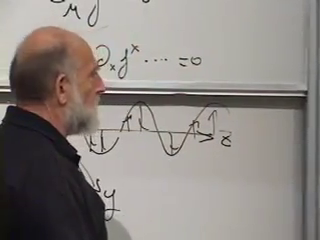
\includegraphics[width=0.70\textwidth]{lecture_58_figure_05.png}
\caption{Schéma complet au tableau d’une onde électromagnétique transverse : les oscillations électrique et magnétique sont perpendiculaires l’une à l’autre et à la direction de propagation.}
\lectureframe{01:05:25}
\end{figure}

\begin{figure}[H]
\centering
\scalebox{0.90}{%
\begin{tikzpicture}[x=1cm,y=1cm,>=Latex]
  \draw[->,thick] (0,0) -- (8.2,0) node[right] {$z$};
  \draw[->,thick] (0,-1.6) -- (0,1.7) node[above] {$x$};
  \draw[->,thick] (0,0) -- (-1.15,-0.8) node[below left] {$y$};
  \draw[blue!70!black,thick,domain=0:7.5,samples=120]
    plot (\x,{0.95*sin(90*\x)});
  \foreach \z/\s in {0.8/1,2.8/-1,4.8/1,6.8/-1}{
    \draw[->,green!45!black,thick]
      (\z,0) -- ++({-0.55*\s},{-0.38*\s});
  }
  \node[blue!70!black] at (6.9,1.25) {$\mathbf E$};
  \node[green!45!black] at (5.2,-1.05) {$\mathbf B$};
  \draw[->,very thick] (6.2,1.55) -- (7.7,1.55)
    node[midway,above] {propagation};
\end{tikzpicture}
}
\caption{Les champs \(\mathbf E\) et \(\mathbf B\) sont perpendiculaires l’un à l’autre et à la direction de propagation.}
\end{figure}

C’est le caractère de la lumière et de tout rayonnement électromagnétique dans le vide. Comme les équations qui produisent l’onde sont covariantes de Lorentz, un autre observateur inertiel décrit lui aussi une onde électromagnétique se déplaçant à \(c\), avec des champs électrique et magnétique transverses.

\section{Densité de charge et densité de courant}

Réintroduisons maintenant les sources que nous avions provisoirement mises de côté. Lorsqu’une région contient de nombreuses particules chargées, il est utile de les décrire à une échelle macroscopique par une densité de charge continue :
\begin{equation}
\rho(\mathbf x,t)=\frac{dQ}{dV}.
\end{equation}
Cette approximation revient à traiter l’eau comme un fluide continu, bien qu’elle soit constituée de molécules. Les charges positives et négatives contribuent avec des signes opposés ; \(\rho\) est donc la charge nette par unité de volume.

La charge contenue dans une région donnée \(V\) est
\begin{equation}
Q_V(t)=\int_V\rho(\mathbf x,t)\,dV.
\label{eq:charge-volume}
\end{equation}
La densité peut varier dans l’espace et au cours du temps. Une accumulation de charges peut quitter un point, ce qui modifie la densité locale à cet endroit. Cette variation ne peut toutefois pas être arbitraire. La nature conserve la charge électrique.

La seule conservation globale serait trop peu contraignante. Elle permettrait à la charge de disparaître de la Terre et de réapparaître sur Mars au même instant, tout en laissant la charge totale inchangée. L’énoncé plus fort est local : la charge ne peut quitter un endroit pour en atteindre un autre qu’en circulant dans l’espace intermédiaire.

Pour décrire cet écoulement, considérons un élément de surface orienté infinitésimal :
\begin{equation}
d\boldsymbol\sigma=\widehat{\mathbf n}\,d\sigma.
\end{equation}
Sa norme est l’aire, et sa direction est normale à la surface. La densité de courant \(\mathbf J\) est définie de sorte que la charge traversant cet élément par unité de temps soit
\begin{equation}
\frac{dQ}{dt}=\mathbf J\cdot d\boldsymbol\sigma.
\label{eq:current-flux-element}
\end{equation}
La norme de \(\mathbf J\) correspond à une charge par unité d’aire et de temps, et sa direction indique le sens d’écoulement des charges positives.

\begin{figure}[H]
\centering
\includegraphics[width=0.64\textwidth]{lecture_58_figure_10.png}
\caption{Élément de surface orienté et facteur de flux \(d\boldsymbol\sigma\cdot\mathbf J\).}
\lectureframe{01:18:15}
\end{figure}

Le produit scalaire sélectionne la composante normale à la surface. Un courant tangent à la surface ne la traverse ni d’un côté ni de l’autre et contribue donc pour zéro. Pour une norme donnée, le courant parallèle à la normale produit le flux maximal. Le courant dans un fil n’est qu’un cas particulier ; \(\mathbf J\) peut aussi décrire un écoulement de charge à travers une feuille ou dans tout un espace tridimensionnel.

\section{Conservation locale et équation de continuité}

Fixons une région \(V\) de l’espace et orientons vers l’extérieur chaque élément de sa frontière fermée \(\partial V\). Si le courant net sortant est positif, la charge contenue dans la région diminue :
\begin{equation}
\frac{dQ_V}{dt}
=-\oint_{\partial V}\mathbf J\cdot d\boldsymbol\sigma.
\label{eq:integral-conservation}
\end{equation}
Le signe moins traduit une réalité physique, il n’est pas dû à une convention : un flux positif sortant retire de la charge positive de la région. En utilisant l’équation~\eqref{eq:charge-volume},
\begin{equation}
\int_V\partial_t\rho\,dV
=-\oint_{\partial V}\mathbf J\cdot d\boldsymbol\sigma.
\label{eq:integral-continuity-one}
\end{equation}

\begin{figure}[H]
\centering
\includegraphics[width=0.72\textwidth]{lecture_58_figure_11.png}
\caption{Loi de conservation dans une région fixe, après conversion du flux à travers la surface en une intégrale de volume.}
\lectureframe{01:29:00}
\end{figure}

Le théorème de Gauss, aussi appelé théorème de la divergence, relie le flux à travers une surface fermée à la divergence à l’intérieur de celle-ci :
\begin{equation}
\oint_{\partial V}\mathbf A\cdot d\boldsymbol\sigma
=\int_V\boldsymbol\nabla\cdot\mathbf A\,dV.
\label{eq:divergence-theorem}
\end{equation}
On peut imaginer des conduits cachés qui injectent de l’eau en différents points à l’intérieur d’un récipient. La divergence mesure le débit local auquel l’eau sort des extrémités des conduits ; l’intégrale de surface mesure la quantité totale d’eau qui quitte le récipient. Toute l’eau qui s’écoule vers l’extérieur depuis l’intérieur doit finir par traverser la frontière.

En appliquant l’équation~\eqref{eq:divergence-theorem} à \(\mathbf J\), on obtient
\begin{equation}
\int_V
\left(\partial_t\rho+\boldsymbol\nabla\cdot\mathbf J\right)dV=0.
\end{equation}
Cette relation vaut pour toute région possible \(V\). L’intégrande doit donc s’annuler en chaque point :
\begin{equation}
\boxed{\partial_t\rho+\boldsymbol\nabla\cdot\mathbf J=0.}
\label{eq:continuity-three}
\end{equation}

\begin{figure}[H]
\centering
\includegraphics[width=0.72\textwidth]{lecture_58_figure_12.png}
\caption{Équation locale de continuité écrite composante par composante.}
\lectureframe{01:29:50}
\end{figure}

L’équation~\eqref{eq:continuity-three} exprime exactement ce qu’exige la conservation locale. Si la densité de charge diminue en un point ou dans une petite région, le courant doit diverger vers l’extérieur. Si le courant converge vers l’intérieur, la densité de charge augmente.

La densité et le courant forment naturellement le quadri-courant
\begin{equation}
J^\mu=(\rho,J_x,J_y,J_z)
\label{eq:four-current}
\end{equation}
dans les unités \(c=1\). L’équation de continuité prend la forme de l’équation scalaire de Lorentz
\begin{equation}
\partial_\mu J^\mu=0.
\label{eq:continuity-four}
\end{equation}
Le flux associé à une distribution relativiste doit se transformer comme un quadrivecteur, tout comme la quadrivitesse d’une particule. L’équation~\eqref{eq:continuity-four} garantit la conservation locale de la charge dans tous les référentiels inertiels.

\section{Les équations de Maxwell avec sources}

En réintroduisant la charge et le courant, on obtient
\begin{align}
\boldsymbol\nabla\cdot\mathbf E&=\rho,
\label{eq:gauss-e-source}\\
\boldsymbol\nabla\cdot\mathbf B&=0,\\
\boldsymbol\nabla\times\mathbf E&=-\partial_t\mathbf B,\\
\boldsymbol\nabla\times\mathbf B&=\partial_t\mathbf E+\mathbf J.
\label{eq:ampere-source}
\end{align}
Les équations faisant intervenir les sources électriques se condensent en
\begin{equation}
\boxed{\partial_\mu F^{\mu\nu}=J^\nu,}
\label{eq:maxwell-source-covariant}
\end{equation}
tandis que la paire magnétique sans source reste
\begin{equation}
\boxed{\partial_\mu\widetilde F^{\mu\nu}=0.}
\label{eq:maxwell-dual-source}
\end{equation}

\begin{figure}[H]
\centering
\includegraphics[width=0.78\textwidth]{lecture_58_figure_13.png}
\caption{Les équations de Maxwell avec sources, accompagnées de leur forme covariante \(\partial_\mu F^{\mu\nu}=J^\nu\).}
\lectureframe{01:34:00}
\end{figure}

La composante temporelle de l’équation~\eqref{eq:maxwell-source-covariant} s’écrit
\begin{equation}
\partial_\mu F^{\mu t}=J^t=\rho,
\end{equation}
et le calcul en composantes déjà effectué transforme son membre de gauche en
\(\boldsymbol\nabla\cdot\mathbf E\). Les trois composantes spatiales redonnent
\(\boldsymbol\nabla\times\mathbf B=\partial_t\mathbf E+\mathbf J\).

On dispose également d’une vérification utile de cohérence. Appliquons \(\partial_\nu\) à l’équation~\eqref{eq:maxwell-source-covariant} :
\begin{equation}
\partial_\nu J^\nu
=\partial_\nu\partial_\mu F^{\mu\nu}=0,
\end{equation}
car les deux dérivées sont symétriques sous l’échange \(\mu\leftrightarrow\nu\), tandis que \(F^{\mu\nu}\) est antisymétrique.\editorialnote{Cette courte vérification de cohérence découle de l’équation covariante et montre explicitement pourquoi les équations de Maxwell avec sources respectent automatiquement l’équation de continuité.}

La structure réciproque est maintenant complète. La loi de force tensorielle
\(f^\mu=qF^\mu{}_\nu u^\nu\)
décrit l’action des champs sur les charges, et l’équation~\eqref{eq:maxwell-source-covariant} décrit comment les charges et les courants produisent les champs. Ces deux relations sont des équations tensorielles. Dans le vide, les mêmes équations de champ conduisent à des ondes transverses se propageant à \(c\). La covariance de Lorentz et l’équation d’onde électromagnétique se rejoignent donc au point qui a motivé toute cette construction : tous les observateurs inertiels obtiennent les mêmes lois de l’électromagnétisme et la même vitesse de la lumière.

\chapter{Temps propre, dilatation du temps et contraction des longueurs}

Nous choisirons souvent des unités dans lesquelles la vitesse de la lumière vaut $c=1$. Dans ces unités, on peut comparer directement une année de temps à une année-lumière de distance, et les formules sont beaucoup plus lisibles. Chaque fois que $c$ intervient physiquement, nous le rétablissons. L’analyse dimensionnelle suffit à le retrouver.

\section{La grille galiléenne de l’espace-temps}

Commençons par la relation pré-einsteinienne entre un référentiel au repos et un train qui se déplace à la vitesse $v$ le long de l’axe $x$ :
\begin{align}
x' &= x-vt, & t'&=t.
\label{eq:l4-galilean}
\end{align}
La deuxième équation exprime l’hypothèse newtonienne d’un temps universel. Tous les observateurs utilisent les mêmes tranches de simultanéité, même si leurs origines spatiales sont en mouvement l’une par rapport à l’autre.

Supposons que l’observateur non primé se trouve à côté de la voie ferrée et que l’observateur primé voyage dans le train. L’origine du train a pour coordonnée $x'=0$ ; sa ligne d’univers dans les coordonnées non primées est donc
\begin{equation}
x=vt.
\end{equation}
Cette droite inclinée est l’axe $t'$. En revanche, $t'=t$ signifie que toutes les lignes de valeur constante de $t'$ sont les mêmes droites horizontales que celles de valeur constante de $t$.

\begin{figure}[H]
\centering
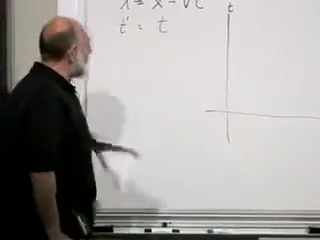
\includegraphics[width=0.72\textwidth]{lecture_04_figure_02.png}
\caption{La transformation galiléenne et la grille initiale $t$-$x$. L’origine mobile décrit $x=vt$, tandis que les deux référentiels conservent des lignes de temps constant communes.}
\lectureframe{00:03:06}
\end{figure}

En résolvant l’équation~\eqref{eq:l4-galilean} par rapport aux coordonnées non primées, on obtient
\begin{align}
x&=x'+vt'=x'+vt, & t&=t'.
\end{align}
La transformation inverse a la même forme, avec $v$ remplacé par $-v$. Si le train avance par rapport à la gare, la gare recule par rapport au train. Cette réciprocité subsiste en relativité restreinte, contrairement au temps universel.

\section{La correction de Lorentz}

Les transformations galiléennes ne peuvent pas rendre la vitesse de la lumière identique dans tous les référentiels inertiels. Les relations corrigées s’écrivent d’abord dans les unités où $c=1$ :
\begin{align}
x'&=\frac{x-vt}{\sqrt{1-v^2}}, &
t'&=\frac{t-vx}{\sqrt{1-v^2}}.
\label{eq:l4-lorentz-natural}
\end{align}
En rétablissant les unités usuelles, on obtient
\begin{align}
x'&=\frac{x-vt}{\sqrt{1-v^2/c^2}}, &
t'&=\frac{t-vx/c^2}{\sqrt{1-v^2/c^2}}.
\label{eq:l4-lorentz-c}
\end{align}

\begin{figure}[H]
\centering
\includegraphics[width=0.74\textwidth]{lecture_04_figure_05.png}
\caption{La transformation de Lorentz avec les facteurs de $c$ rétablis.}
\lectureframe{00:09:10}
\end{figure}

Pour $v\ll c$, $v^2/c^2$ et $vx/c^2$ sont tous deux très petits dans les situations où l’on utilise la mécanique newtonienne. L’équation~\eqref{eq:l4-lorentz-c} se réduit alors au résultat galiléen. La relativité n’abandonne pas la cinématique newtonienne ; elle en délimite le domaine de validité.

Pour $v=c$, le dénominateur s’annule. Un référentiel inertiel ne peut pas se déplacer à la vitesse de la lumière par rapport à un autre référentiel inertiel. Bien en dessous de cette limite, les corrections sont faibles, mais à proximité, le mélange de $x$ et de $t$ devient inévitable.

Le mouvement étant choisi selon $x$, les coordonnées transversales ne changent pas :
\begin{equation}
y'=y,\qquad z'=z.
\end{equation}
On peut comprendre pourquoi en plaçant des règles identiques dans la direction transversale, l’une dans le train et l’autre sur le quai. Un observateur se déplaçant à mi-chemin entre les deux référentiels voit les règles s’approcher à des vitesses égales et opposées. Rien dans cette configuration ne peut faire paraître l’une des règles transversales plus courte que l’autre.

\section{Transformations de Lorentz le long du cône de lumière}

L’équation~\eqref{eq:l4-lorentz-natural} se prête à une lecture géométrique. Additionnons ses deux équations :
\begin{align}
t'+x'
&=\frac{(t-vx)+(x-vt)}{\sqrt{1-v^2}}\\
&=(t+x)\frac{1-v}{\sqrt{1-v^2}}\\
&=(t+x)\sqrt{\frac{1-v}{1+v}}.
\label{eq:l4-null-plus}
\end{align}
Soustrayons-les dans l’ordre inverse :
\begin{align}
t'-x'
&=\frac{(t-vx)-(x-vt)}{\sqrt{1-v^2}}\\
&=(t-x)\frac{1+v}{\sqrt{1-v^2}}\\
&=(t-x)\sqrt{\frac{1+v}{1-v}}.
\label{eq:l4-null-minus}
\end{align}

\begin{figure}[H]
\centering
\includegraphics[width=0.75\textwidth]{lecture_04_figure_06.png}
\caption{La transformation de Lorentz réécrite à l’aide des combinaisons nulles $t+x$ et $t-x$. Leurs facteurs d’échelle sont inverses l’un de l’autre.}
\lectureframe{00:18:45}
\end{figure}

Les combinaisons $t+x$ et $t-x$ sont des coordonnées le long des deux directions de lumière à $45^\circ$. Un boost comprime l’une de ces directions et étire l’autre selon le facteur inverse. Il n’écarte ni l’une ni l’autre de $45^\circ$. Ainsi, les rayons lumineux restent des rayons lumineux : c’est la représentation de l’invariance de la vitesse de la lumière dans l’espace-temps.

\begin{classroomqa}\audiencequestion{L’observateur à mi-chemin voit une expérience symétrique, mais en quoi cela établit-il le résultat pour les observateurs du train et du quai ?\lecturetimestamp{00:20:48}}\lecturerresponse{On fait appel à un fait supplémentaire : la coïncidence de deux événements est invariante. Si les extrémités des règles se rencontrent, cette rencontre constitue un événement unique dans l’espace-temps. Chaque observateur inertiel peut lui attribuer des coordonnées différentes, mais aucun ne peut scinder une coïncidence en deux lieux distincts. Des éclairs émis au point de rencontre des extrémités correspondantes rendent ces événements détectables expérimentalement. La symétrie dans le référentiel à mi-chemin et l’invariance des deux coïncidences aux extrémités établissent l’égalité des longueurs transversales.}
\end{classroomqa}

\begin{classroomqa}\audiencequestion{Le cycliste qui représente le référentiel à mi-chemin doit-il se trouver physiquement au milieu des règles ?\lecturetimestamp{00:22:25}}\lecturerresponse{Non. Un référentiel est un réseau entier d’observateurs et d’horloges, pas un œil placé en un point donné. Le cycliste peut recevoir plus tard les éclairs émis aux extrémités et déduire leur lieu d’émission. Ce qui compte, c’est la position dans l’espace-temps de chaque événement d’émission, et non le lieu où la lumière est finalement reçue.}
\end{classroomqa}

La composition de vitesses successives est une autre conséquence de cette même transformation, mais nous la réserverons délibérément au cours suivant. Pour l’instant, il s’agit d’identifier la grandeur invariante mesurée par une horloge en mouvement.

\section{L’intervalle invariant}

Pour une rotation des axes cartésiens usuels, la grandeur $x^2+y^2$ reste inchangée. Les transformations de Lorentz conservent une autre forme quadratique. D’après l’équation~\eqref{eq:l4-lorentz-natural},
\begin{align}
t'^2-x'^2
&=\frac{(t-vx)^2-(x-vt)^2}{1-v^2}\\
&=\frac{t^2-2vtx+v^2x^2-x^2+2vtx-v^2t^2}{1-v^2}\\
&=t^2-x^2.
\label{eq:l4-interval}
\end{align}
Les termes croisés s’annulent, et le numérateur restant contient le facteur commun $1-v^2$.

\begin{figure}[H]
\centering
\includegraphics[width=0.76\textwidth]{lecture_04_figure_07.png}
\caption{La dérivation au tableau de $t'^2-x'^2=t^2-x^2$.}
\lectureframe{00:33:15}
\end{figure}

Avec trois dimensions spatiales, l’invariant est
\begin{equation}
t'^2-x'^2-y'^2-z'^2=t^2-x^2-y^2-z^2
\end{equation}
dans les unités où $c=1$. Plus généralement, pour deux événements, nous utilisons les différences de coordonnées :
\begin{equation}
\Delta s^2
=c^2\Delta t^2-\Delta x^2-\Delta y^2-\Delta z^2.
\label{eq:l4-spacetime-interval}
\end{equation}
Tous les observateurs inertiels s’accordent sur cette valeur, même s’ils ne s’accordent pas sur ses termes temporel et spatial pris séparément.

\section{Temps propre et horloges en mouvement}

Imaginons un réseau d’observateurs immobiles dont les horloges ont été synchronisées par échange de signaux lumineux. Leurs indications définissent le temps coordonné $t$. Transportons maintenant une montre-bracelet à travers ce réseau. Son indication propre accompagne la montre le long de sa ligne d’univers : c’est le temps propre.

Pour deux événements séparés par un intervalle de genre temps, définissons
\begin{equation}
c^2\Delta\tau^2
=c^2\Delta t^2-\Delta x^2-\Delta y^2-\Delta z^2.
\label{eq:l4-proper-time}
\end{equation}
Dans une dimension spatiale et avec $c=1$, cela donne simplement
\begin{equation}
\Delta\tau=\sqrt{\Delta t^2-\Delta x^2}.
\end{equation}
La racine carrée rappelle la formule de la distance usuelle, mais le signe moins change la géométrie.

Il y a trois cas :
\begin{align}
\Delta t^2-\Delta x^2 &>0 &&\text{timelike},\\
\Delta t^2-\Delta x^2 &=0 &&\text{lightlike},\\
\Delta t^2-\Delta x^2 &<0 &&\text{spacelike}.
\end{align}
À l’intérieur du cône de lumière, le temps propre est réel. Sur le cône, où $x=\pm t$, il est nul, même si les événements ne coïncident pas. Un rayon lumineux peut relier précisément de tels événements. À l’extérieur du cône, la séparation est de genre espace ; il vaut mieux la décrire par la distance propre réelle $\sqrt{\Delta x^2-\Delta t^2}$ que par un temps d’horloge imaginaire.

\begin{figure}[H]
\centering
\includegraphics[width=0.73\textwidth]{lecture_04_figure_08.png}

\vspace{0.8em}

\begin{tikzpicture}[x=1.0cm,y=1.0cm]
\draw[->] (-3.3,0) -- (3.3,0) node[right] {$x$};
\draw[->] (0,-0.4) -- (0,4.0) node[above] {$t$};
\draw[thick] (0,0) -- (3.0,3.0) node[above right] {$x=t$};
\draw[thick] (0,0) -- (-3.0,3.0) node[above left] {$x=-t$};
\node at (0,2.0) {timelike};
\node at (2.25,1.05) {spacelike};
\node at (-2.25,1.05) {spacelike};
\end{tikzpicture}\caption{Le cône de lumière au tableau et une classification claire des séparations de genre temps, de genre lumière et de genre espace.}
\lectureframe{00:38:40}
\end{figure}

Pourquoi l’équation~\eqref{eq:l4-proper-time} donne-t-elle l’indication d’une horloge ? Pour une horloge au repos, $\Delta x=0$, donc $\Delta\tau=\Delta t$. Pour une horloge en mouvement uniforme, choisissons le référentiel primé dans lequel elle est au repos. Dans ce référentiel, $\Delta x'=0$, et l’invariance donne
\begin{equation}
\Delta\tau
=\sqrt{\Delta t'^2-\Delta x'^2}
=\Delta t'.
\end{equation}
Les horloges en mouvement mesurent donc le temps propre.

\begin{classroomqa}\audiencequestion{``l’intervalle entre les événements'' et ``l’indication de l’horloge'' sont-ils deux noms pour une même chose ?\lecturetimestamp{00:44:49}}\lecturerresponse{Ils coïncident lorsqu’une horloge idéale se déplace inertiellement d’un événement à l’autre. L’intervalle invariant est une grandeur géométrique ; la différence entre les indications de l’horloge comobile aux deux extrémités en est la mesure physique. Une horloge coordonnée immobile enregistre généralement un intervalle de temps coordonné différent.}
\end{classroomqa}

\section{Dilatation du temps et simultanéité}

Considérons l’origine du référentiel en mouvement. Sa ligne d’univers vérifie
\begin{equation}
x'=0,\qquad x=vt.
\end{equation}
Cette même droite inclinée est à la fois la trajectoire de l’horloge mobile et l’axe $t'$.

\begin{figure}[H]
\centering
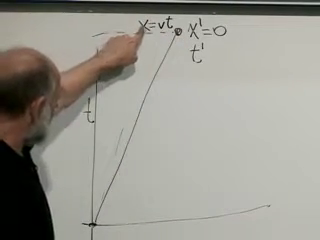
\includegraphics[width=0.72\textwidth]{lecture_04_figure_03.png}
\caption{L’origine mobile : $x=vt$, $x'=0$ et l’axe $t'$ sont trois descriptions d’une même ligne d’univers.}
\lectureframe{00:48:18}
\end{figure}

Appliquons l’intervalle invariant entre l’origine commune et un point ultérieur de cette ligne d’univers :
\begin{align}
t'^2-x'^2&=t^2-x^2,\\
t'^2&=t^2-v^2t^2,\\
t'&=t\sqrt{1-v^2}.
\label{eq:l4-time-dilation-natural}
\end{align}
En rétablissant $c$,
\begin{equation}
\Delta\tau=\Delta t\sqrt{1-\frac{v^2}{c^2}}
=\frac{\Delta t}{\gamma},
\qquad
\gamma=\frac{1}{\sqrt{1-v^2/c^2}}.
\label{eq:l4-time-dilation}
\end{equation}

\begin{figure}[H]
\centering
\includegraphics[width=0.73\textwidth]{lecture_04_figure_09.png}
\caption{Le résultat de dilatation du temps au tableau : l’horloge mobile accumule $t'=t\sqrt{1-v^2}$ dans les unités où $c=1$.}
\lectureframe{00:50:45}
\end{figure}

L’observateur immobile dit que l’horloge mobile retarde. Par réciprocité, l’observateur mobile doit dire la même chose des horloges immobiles. Il n’y a pas de contradiction, car les deux descriptions comparent des paires différentes d’événements éloignés.

En effet, une valeur constante de $t'$ dans l’équation~\eqref{eq:l4-lorentz-natural} vérifie
\begin{equation}
t-vx=\text{constant}.
\label{eq:l4-simultaneity}
\end{equation}
Les lignes de simultanéité de l’observateur mobile sont inclinées par rapport aux lignes horizontales $t=\text{constant}$. Chaque observateur considère comme simultanés des ensembles différents d’indications d’horloges éloignées. Dès lors que cette différence reste présente à l’esprit, le ralentissement réciproque des horloges est cohérent.

\begin{figure}[H]
\centering
\begin{tikzpicture}[x=1cm,y=1cm]
\draw[->] (0,0) -- (0,4.2) node[above] {$t$};
\draw[->] (0,0) -- (5.2,0) node[right] {$x$};
\draw[thick,->] (0,0) -- (2.4,3.8) node[above] {$x'=0$};
\draw[dashed] (0,2.8) -- (4.8,2.8)
  node[right] {$t=\mathrm{const}$};
\draw[thick] (0.15,1.05) -- (4.7,2.35)
  node[right] {$t'=\mathrm{const}$};
\draw[thick] (3.4,0) -- (3.4,3.8);
\fill (3.4,2.8) circle (0.045);
\fill (3.4,1.98) circle (0.045);
\end{tikzpicture}
\caption{La dilatation réciproque du temps compare des indications d’horloges sur des tranches de simultanéité différentes.}
\end{figure}

\section{Les trajectoires des jumeaux}

Deux jumeaux partent du même événement. L’un reste en $x=0$. L’autre s’éloigne à la vitesse $v$, fait demi-tour et revient à la même vitesse. Lorsqu’ils se retrouvent, ils comparent tous les processus physiques pouvant servir d’horloge : montres, battements du cœur, métabolisme ou vieillissement lui-même.

Supposons que chaque moitié du voyage dure $T$ en temps coordonné dans le référentiel du jumeau resté chez lui. Son temps propre est
\begin{equation}
\tau_{\mathrm{home}}=2T.
\end{equation}
L’événement du demi-tour a pour coordonnées $(vT,T)$. La première étape du voyage contribue donc à
\begin{align}
\tau_{\mathrm{leg}}
&=\sqrt{T^2-v^2T^2}
=T\sqrt{1-v^2}.
\end{align}
L’étape du retour apporte la même durée, d’où
\begin{equation}
\tau_{\mathrm{travel}}=2T\sqrt{1-v^2}<2T.
\label{eq:l4-twin}
\end{equation}

\begin{figure}[H]
\centering
\includegraphics[width=0.73\textwidth]{lecture_04_figure_10.png}

\vspace{0.8em}

\begin{tikzpicture}[x=1.1cm,y=1cm]
\draw[->] (-0.2,0) -- (3.4,0) node[right] {$x$};
\draw[->] (0,-0.1) -- (0,4.4) node[above] {$t$};
\draw[very thick] (0,0) -- (0,4);
\draw[very thick] (0,0) -- (2.2,2) -- (0,4);
\draw[dashed] (0,2) -- (2.2,2);
\node[left] at (0,2) {$T$};
\node[left] at (0,4) {$2T$};
\node[below right] at (1.1,1.0) {$v$};
\node[above right] at (1.1,3.0) {$-v$};
\end{tikzpicture}\caption{La ligne d’univers du jumeau resté chez lui et les deux étapes du voyage. Leurs temps propres diffèrent parce que leurs trajectoires dans l’espace-temps sont différentes.}
\lectureframe{00:59:35}
\end{figure}

L’inégalité des âges n’a rien de contradictoire. La trajectoire du voyageur comporte un demi-tour et n’est pas liée à la ligne droite du jumeau resté chez lui par une unique symétrie de référentiel inertiel. En géométrie euclidienne ordinaire, un trajet rectiligne et un trajet brisé entre deux points ont également des longueurs différentes. La géométrie de Minkowski inverse la trajectoire dont l’intervalle est le plus grand, mais la comparaison reste géométrique.

\section{Accélération et horloge idéale}

\begin{classroomqa}\audiencequestion{Au moment du demi-tour, la situation physique est différente et le voyageur accélère. Cela invalide-t-il le calcul des horloges ?\lecturetimestamp{01:02:19}}\lecturerresponse{L’accélération est réelle et contribue à révéler l’asymétrie ; il ne faut pas chercher à l’écarter du raisonnement. Le coin pointu n’est qu’une représentation idéalisée et peut être arrondi en un demi-tour de durée finie. L’autre hypothèse physique est qu’une horloge suffisamment petite et bien conçue est insensible à une accélération modérée et continue de mesurer le temps propre. Une horloge grande ou fragile risque de se déformer ou de se briser, mais ce serait un défaut de son mécanisme, et non de l’intervalle d’espace-temps.}
\end{classroomqa}

Cette hypothèse de l’horloge idéale ne découle pas de la seule transformation de Lorentz. Elle est mise à l’épreuve par le comportement des mécanismes d’horlogerie réels. Un atome en constitue une bien meilleure approximation qu’une horloge large de plusieurs centaines de miles, car un mécanisme compact est plus difficile à déformer sous l’effet de l’accélération ou de la gravité. Invoquer la relativité générale ne résoudrait pas cette difficulté physique : il faudrait toujours savoir comment le mécanisme choisi réagit à son environnement.

\begin{classroomqa}\audiencequestion{Peut-on décomposer une trajectoire accélérée en courts intervalles sur lesquels l’analyse inertielle reste valable ?\lecturetimestamp{01:09:08}}\lecturerresponse{Oui. Découpons la courbe en segments courts, presque rectilignes, calculons le temps propre sur chaque segment, puis additionnons les résultats. C’est l’analogue dans l’espace-temps du calcul de la longueur d’une courbe ordinaire à partir d’une multitude de petits segments de droite. À la limite continue,
\[
\tau=\int \sqrt{1-\frac{v(t)^2}{c^2}}\,dt,
\]
pour un mouvement dans un espace-temps plat décrit dans un système de coordonnées inertiel.}
\end{classroomqa}

\section{Ce que voient les jumeaux}

On peut rendre opérationnelles les indications finales des horloges en envoyant des impulsions lumineuses. Marquons des intervalles de temps propre d’une seconde sur les deux lignes d’univers et faisons émettre une impulsion par chaque jumeau à chaque marque. Pendant l’étape de l’aller, les impulsions reçues de l’autre jumeau sont de plus en plus espacées. Au retour, elles arrivent de plus en plus rapprochées. C’est l’effet Doppler relativiste représenté directement sur le diagramme d’espace-temps.

\begin{figure}[H]
\centering
\includegraphics[width=0.73\textwidth]{lecture_04_figure_11.png}
\caption{Signaux lumineux échangés entre la ligne d’univers du jumeau resté chez lui et celle du voyageur. Les arrivées espacées pendant l’aller puis rapprochées pendant le retour rendent compte de toutes les impulsions émises.}
\lectureframe{01:12:55}
\end{figure}

Aucune partie de l’histoire ne disparaît. Chaque observateur finit par recevoir toutes les impulsions émises par l’autre, mais leur fréquence de réception dépend du mouvement relatif. Les effets de décalage vers le rouge à l’aller et vers le bleu au retour n’ont pas la même durée pour les deux trajectoires ; le décompte de toutes les impulsions reçues concorde donc avec la comparaison des temps propres.

\begin{classroomqa}\audiencequestion{Si le voyageur de retour reçoit une lumière décalée vers le bleu, pourrait-il recueillir plus d’énergie que la source n’en a émise ?\lecturetimestamp{01:13:50}}\lecturerresponse{Pour répondre, il faut avoir développé la définition relativiste de l’énergie et sa dépendance au référentiel. La question est légitime, mais les coordonnées et le décompte des impulsions ne suffisent pas à établir le bilan énergétique, surtout pour un observateur accéléré. Il vaut donc mieux différer la réponse que la deviner.}
\end{classroomqa}

\section{Une direction spatiale fermée}

\begin{classroomqa}\audiencequestion{Supposons qu’une direction spatiale soit compacte. Un jumeau pourrait-il s’y déplacer uniformément, revenir à son point de départ et éviter toute accélération ? Qu’est-ce qui distinguerait alors les jumeaux ?\lecturetimestamp{01:15:14}}\lecturerresponse{Il faut concevoir l’espace intrinsèquement comme un cylindre, et non comme une feuille courbée dans un espace plus vaste ; il n’y a pas nécessairement d’accélération radiale. L’observateur qui revient rencontre néanmoins le fait global que les mêmes lieux se répètent. Cela indique une asymétrie, mais une réponse complète exige un traitement rigoureux de la relativité restreinte avec l’identification spatiale. Nous laissons ici la question ouverte au lieu d’improviser une réponse.}
\end{classroomqa}

\begin{figure}[H]
\centering
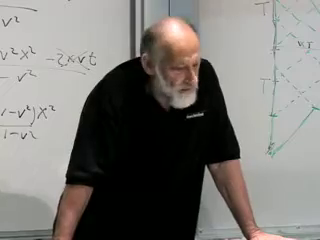
\includegraphics[width=0.72\textwidth]{lecture_04_figure_04.png}

\vspace{0.8em}

\begin{tikzpicture}[x=1cm,y=1cm]
\draw[thick] (0,0) ellipse (1.3 and 0.35);
\draw[thick] (-1.3,0) -- (-1.3,-3.1);
\draw[thick] (1.3,0) -- (1.3,-3.1);
\draw[thick] (0,-3.1) ellipse (1.3 and 0.35);
\draw[->,very thick] (0.0,0.38) arc (90:-210:1.38 and 0.42);
\node[right] at (1.65,-1.5) {compact spatial direction};
\end{tikzpicture}\caption{La question de l’espace compact telle qu’elle est dessinée au tableau, avec un cylindre intrinsèque net. Elle porte sur une identification globale, et non sur un mouvement autour d’un cylindre plongé dans une dimension radiale supplémentaire.}
\lectureframe{01:17:56}
\end{figure}

\section{La longueur se mesure sur une tranche de simultanéité}

Pour un problème de relativité restreinte, commençons par dessiner le diagramme d’espace-temps. Prenons une règle d’un mètre au repos dans le référentiel non primé, dont les extrémités se trouvent en $x=0$ et $x=1$. Au fil du temps, les deux extrémités décrivent des lignes d’univers verticales. La règle balaie un ruban dans l’espace-temps.

L’observateur mobile doit mesurer les deux extrémités à une même valeur du temps mobile $t'$. D’après l’équation~\eqref{eq:l4-simultaneity}, la tranche qui passe par l’origine et vérifie $t'=0$ satisfait
\begin{equation}
t=vx
\end{equation}
dans les unités où $c=1$. Elle coupe la ligne d’univers de l’extrémité droite $x=1$ en $t=v$.

\begin{figure}[H]
\centering
\includegraphics[width=0.73\textwidth]{lecture_04_figure_12.png}

\vspace{0.8em}

\begin{tikzpicture}[x=1.55cm,y=1.15cm]
\draw[->] (-0.5,0) -- (3.1,0) node[right] {$x$};
\draw[->] (0,0) -- (0,3.8) node[above] {$t$};
\draw[very thick,red] (0,0) -- (0,3.3);
\draw[very thick,red] (2.15,0) -- (2.15,3.3);
\fill[red!12] (0,0) rectangle (2.15,3.3);
\draw[very thick,green!50!black] (0,0) -- (1.2,3.1)
  node[above] {$x=vt$};
\draw[very thick,blue] (0,0) -- (2.15,1.15)
  node[right] {$t'=0$};
\fill (2.15,1.15) circle (0.045);
\node[right] at (2.22,1.35) {$(x,t)=(1,v)$};
\node[below] at (2.15,0) {$1$};
\end{tikzpicture}\caption{Une règle au repos balaie un ruban dans l’espace-temps. Pour l’observateur mobile, la longueur est la distance entre ses extrémités sur une tranche $t'=\mathrm{const}$.}
\lectureframe{01:24:20}
\end{figure}

La séparation choisie entre les extrémités est de genre espace ; utilisons donc la forme spatiale positive de l’invariant :
\begin{equation}
x'^2-t'^2=x^2-t^2.
\end{equation}
À l’extrémité choisie, $t'=0$, $x=1$ et $t=v$. On a donc
\begin{align}
x'^2&=1-v^2,\\
x'&=\sqrt{1-v^2}.
\end{align}
Ainsi, une longueur au repos $L$ est mesurée dans le référentiel mobile comme
\begin{equation}
L'=L\sqrt{1-v^2/c^2}=\frac{L}{\gamma}.
\label{eq:l4-length-contraction}
\end{equation}

\begin{figure}[H]
\centering
\includegraphics[width=0.76\textwidth]{lecture_04_figure_13.png}
\caption{La construction complète de la contraction des longueurs et le résultat au tableau $x'=\sqrt{1-v^2}$ pour une longueur au repos unitaire.}
\lectureframe{01:28:10}
\end{figure}

La réciproque est également vraie : l’observateur sur le quai attribue une longueur plus courte à la règle longitudinale d’un mètre du train. Une fois encore, les deux observateurs choisissent des événements simultanés différents aux extrémités, si bien que cette réciprocité n’est pas contradictoire.

\section{Questions de fin de cours}

\begin{classroomqa}
\audiencequestion{À part la lumière, quelque chose se propage-t-il à la vitesse de la lumière ? Qu’en est-il en particulier de la gravité ?\lecturetimestamp{01:29:29}}
\lecturerresponse{La relativité générale prédit que les ondes gravitationnelles se propagent à $c$. À l’époque de ce cours, les indices étaient indirects et provenaient de systèmes tels que les pulsars binaires ; les ondes gravitationnelles n’avaient pas encore été détectées directement.\editorialnote{La situation expérimentale a changé après ce cours de 2006. LIGO a détecté directement GW150914 en 2015, et l’observation conjointe de GW170817 et de son homologue électromagnétique en 2017 a montré que les vitesses de propagation de la gravité et de la lumière concordent à quelques parties près sur $10^{15}$. Voir \url{https://ligo.org/detections/gw150914/} et
\url{https://doi.org/10.1103/PhysRevLett.119.251302}.}}
\end{classroomqa}

\begin{classroomqa}\audiencequestion{Un astronaute peut-il parcourir une distance de plusieurs années-lumière en un temps propre inférieur à cette distance exprimée en années-lumière ? Cela signifierait-il qu’il se déplace plus vite que la lumière ?\lecturetimestamp{01:30:38}}\lecturerresponse{Le temps propre de l’astronaute est $\sqrt{\Delta t^2-\Delta x^2}$, une durée inférieure au temps coordonné $\Delta t$. Dans le référentiel inertiel de l’astronaute, la distance entre les étoiles est contractée par Lorentz. Les étoiles se déplacent à la vitesse $-v$, et non plus vite que la lumière ; la distance à parcourir est simplement plus courte après contraction.}
\end{classroomqa}

Si l’astronaute part du repos et accélère, la description change au fil d’une succession de référentiels inertiels instantanés. La distance attribuée aux étoiles peut varier pendant cette transition. On ne peut pas appliquer une unique transformation de Lorentz à toute l’histoire accélérée, mais le temps propre total s’obtient toujours en additionnant les contributions le long de la ligne d’univers. Il en va de même pour un jumeau réaliste qui démarre, fait demi-tour et décélère, au lieu de naître à la vitesse de croisière.

\begin{classroomqa}\audiencequestion{Ces paradoxes viennent-ils du fait que le temps est traité comme une notion particulière ? Faut-il parler d’une quatrième dimension ?\lecturetimestamp{01:36:43}}\lecturerresponse{Il n’est pas nécessaire de commencer par affirmer que le temps est une quatrième dimension. La transformation de Lorentz impose à elle seule le mélange de l’espace et du temps, tandis que l’intervalle $t^2-x^2-y^2-z^2$ les traite comme des composantes d’une même géométrie, avec un signe différent pour le temps et pour l’espace. À faible vitesse, le mélange devient négligeable et l’intuition newtonienne familière reprend ses droits. Aux vitesses relativistes, en revanche, on ne peut pas considérer l’espace et le temps comme fondamentalement découplés.}
\end{classroomqa}

La dilatation du temps, la contraction des longueurs, la comparaison des jumeaux et la réduction du temps de voyage ne sont donc pas des astuces distinctes. Elles découlent toutes de trois habitudes : repérer les événements comparés, représenter leur géométrie dans l’espace-temps et utiliser l’intervalle invariant.
\chapter{Boules de feu, référentiels et quadrivecteurs}

Nous partons d’une question laissée en suspens après la discussion des collisions à haute énergie. La collision de deux noyaux lourds crée un objet qui évolue violemment, et non un trou noir astronomique au repos. Que peut donc signifier décrire la collision au moyen d’un horizon ? La réponse passe par une représentation en cinq dimensions de la matière fortement couplée, par quelques questions pratiques sur les accélérateurs, puis nous ramène à la géométrie de la relativité restreinte. À la fin, vitesse et quantité de mouvement sont devenues des quadrivecteurs, et l’énergie a pris place aux côtés des trois composantes de la quantité de mouvement.

\section{Une boule de feu dans une cinquième dimension}

\begin{classroomqa}\audiencequestion{L’objet produit par la collision est instable et change de forme. Comment peut-on appeler trou noir un objet aussi complexe ?}\lecturerresponse{Imaginons une cinquième direction spatiale qui s’étend entre un plancher et un plafond. La gravité dans cette direction attire les excitations vers le plancher. La collision y dépose une masse d’énergie chaude ; celle-ci s’étale et change de forme, mais elle peut tout de même posséder un horizon, une température et une entropie.}\end{classroomqa}

Imaginons des particules — ou, de façon plus imagée, de petites cordes — qui se déplacent dans ce monde à cinq dimensions. Les excitations qui tombent vers le plancher apparaissent en quatre dimensions sous la forme de hadrons : protons, neutrons, mésons et autres objets composites étendus. Celles qui restent près du plafond paraissent plus élémentaires. La position verticale fournit donc une manière géométrique d’encoder l’échelle : le plancher représente le régime hadronique à longue distance, tandis que le plafond représente les degrés de liberté à courte distance.

Lorsque deux hadrons entrent en collision, deux objets proches du plancher se heurtent et produisent une grande gerbe d’énergie. Le résultat n’est pas un corps rigide. C’est une masse chaude dotée d’un horizon, une sorte de flaque dans le champ gravitationnel à cinq dimensions. Ce n’est ni un trou noir astronomique dans l’espace ordinaire à quatre dimensions, ni un trou noir à l’échelle de Planck fixé au plafond. C’est la description gravitationnelle de la boule de feu fortement couplée près du plancher.

À haute énergie, les noyaux incidents sont contractés par effet Lorentz en fines crêpes. Ils entrent en collision, déposent leur énergie dans une petite région et produisent un fluide qui évolue vers l’équilibre. Sa faible viscosité était l’une des propriétés surprenantes du plasma de quarks--gluons. Dans la description à cinq dimensions, cette même évolution correspond à la relaxation d’un horizon déformé.

\begin{figure}[H]\centering
\includegraphics[width=0.82\textwidth]{lecture_05_figure_01.png}\caption{Représentation de la cinquième dimension par un plancher et un plafond. Après la collision, la masse centrale dotée d’un horizon s’étale le long du plancher.}\lectureframe{00:04:22}\end{figure}

Un horizon ne persiste pas éternellement. Le rayonnement de Hawking emporte de l’énergie ; dans la description à quatre dimensions, ce rayonnement est la gerbe de hadrons ordinaires qui émergent de la collision. Dans ce langage, les milliers de traces d’un événement détecté sont les particules émises par le trou noir dual, comme si elles en avaient bouilli.

\subsection{La dimension supplémentaire est-elle réelle ?}

\begin{classroomqa}\audiencequestion{La cinquième dimension est-elle une dimension spatiale, et la ligne tracée entre le plancher et le plafond s’étend-elle littéralement dans cette direction ?}\lecturerresponse{Oui. Elle est de genre espace, et la surface représentée dans cette géométrie à cinq dimensions est un horizon. La question de savoir si l’on peut appeler cette direction supplémentaire ``réelle'' ou si l’on doit la considérer comme une description mathématique équivalente est plus profonde.}\end{classroomqa}

L’idée utile n’est pas que la gravité remplace la chromodynamique quantique. Deux langages peuvent plutôt décrire la même physique. Dans le langage à quatre dimensions, il y a une boule de feu chaude de quarks et de gluons, sans champ gravitationnel ordinaire. Dans celui à cinq dimensions, il y a la gravité et un horizon. Si la correspondance est correcte, un calcul rigoureux en QCD et le calcul gravitationnel dual doivent coïncider partout où les deux peuvent être effectués.

\begin{classroomqa}\audiencequestion{La QCD ne comporte ni gravité ni horizon. L’image du trou noir ajoute-t-elle une nouvelle physique, ou ne fait-elle que redécrire la boule de feu ?}\lecturerresponse{En quatre dimensions, c’est un plasma de quarks et de gluons ; dans son incarnation à cinq dimensions, elle possède une description gravitationnelle avec un horizon. L’avantage est d’ordre calculatoire. La QCD fortement couplée est extrêmement difficile à traiter, tandis que certaines propriétés de l’horizon---en particulier la viscosité---sont relativement faciles à calculer.}\end{classroomqa}

Il n’est pas nécessaire de trancher la distinction entre ``dimension réelle'' et ``analogie mathématique'' pour que la description soit utile. Une structure acquiert une interprétation physique lorsqu’elle réunit les autres variables au sein d’un ensemble de lois plus simple et plus cohérent. Il ne faut toutefois pas exagérer la portée de l’argument : les applications de la dualité jauge-gravité au plasma de quarks--gluons observé sont des modèles de dynamique fortement couplée, et non la preuve que la QCD du monde réel possède un dual gravitationnel exact connu.\editorialnote{Cette précision explicite le statut actuel de l’application à la QCD ; elle ne modifie pas le mécanisme à cinq dimensions développé ici.}

\section{Pourquoi faire entrer en collision des faisceaux dans les collisionneurs}

Les questions deviennent maintenant pratiques. Pourquoi utiliser deux faisceaux en mouvement plutôt qu’un seul faisceau et une cible immobile ? Pourquoi les accélérateurs circulaires sont-ils si grands ? Pourquoi traite-t-on différemment les électrons et les protons ? Toutes ces questions portent sur l’énergie relativiste.

\begin{classroomqa}\audiencequestion{Pourquoi faire entrer en collision deux faisceaux plutôt que d’envoyer un faisceau énergétique sur une cible immobile ?}\lecturerresponse{Ce qui crée de nouvelles particules, c’est l’énergie disponible dans le référentiel du centre de masse. Deux faisceaux relativistes égaux et opposés ont une quantité de mouvement totale nulle ; leur énergie est donc pratiquement entièrement disponible pour la collision. Avec une cible fixe, une grande partie de l’énergie incidente reste sous forme de mouvement du centre de masse.}\end{classroomqa}

Pour deux particules ultrarelativistes de quantités de mouvement opposées, de norme \(p\), l’estimation donnée au niveau du cours, en unités \(c=1\), est
\begin{equation}
E_{\mathrm{cm}}^{\mathrm{collider}}\simeq 2p.
\end{equation}
L’estimation correspondante pour une cible fixe ne croît que comme la racine carrée de la quantité de mouvement du faisceau,
\begin{equation}
E_{\mathrm{cm}}^{\mathrm{fixed}}\sim \sqrt{mp}.
\end{equation}
C’est la loi d’échelle qui importe, et non le facteur numérique omis : doubler l’énergie du faisceau double l’énergie dans le collisionneur, mais n’augmente l’énergie dans le référentiel du centre de masse que comme une racine carrée pour une cible fixe.

Le calcul invariant permet de préciser la comparaison. Si \(P_1\) et \(P_2\) sont les quadrimpulsions incidentes, alors
\begin{equation}
s=(P_1+P_2)^2,
\qquad E_{\mathrm{cm}}=\sqrt{s}.
\end{equation}
Pour deux faisceaux égaux et se propageant en sens opposés, d’énergie \(E\), les quantités de mouvement spatiales se compensent et \(\sqrt{s}=2E\). Pour un projectile d’énergie \(E\gg m\) qui frappe une cible au repos de même masse,
\begin{equation}
s=2m^2+2mE,
\qquad
\sqrt{s}\simeq \sqrt{2mE}
\qquad (c=1).
\end{equation}
Cette courte dérivation à partir d’invariants fournit le facteur omis dans l’estimation orale.\editorialnote{Elle est incluse pour que l’on puisse retrouver la loi d’échelle présentée dans le cours.}

\begin{classroomqa}\audiencequestion{Y a-t-il une raison fondamentale pour qu’un accélérateur circulaire soit si grand ? Le même faisceau ne pourrait-il pas simplement circuler davantage de fois dans une machine plus petite ?}\lecturerresponse{Les champs et les matériaux imposent des limites. Une particule ne gagne qu’une quantité finie d’énergie par mètre ; une machine plus énergétique doit donc disposer d’une plus grande longueur d’accélération effective. Un anneau étroit exige également une accélération transverse plus importante, et une charge accélérée rayonne. Si l’anneau est trop petit, le faisceau rayonne de l’énergie aussi vite que la machine la lui fournit.}\end{classroomqa}

La relation de courbure est approximativement
\begin{equation}
p=qBR,
\end{equation}
Ainsi, à champ magnétique \(B\) fixé, une quantité de mouvement \(p\) plus grande exige un rayon \(R\) plus grand. Les cavités radiofréquence fournissent le travail qui augmente l’énergie du faisceau ; les aimants courbent et focalisent le faisceau. La conclusion générale reste celle formulée au tableau : l’intensité des champs et les pertes radiatives nous empêchent de réduire à volonté un accélérateur d’énergie arbitrairement élevée à un petit anneau.

Un mouvement circulaire comporte une accélération même à vitesse constante, car la vitesse change de direction. Une charge accélérée émet un rayonnement synchrotron. Un accélérateur linéaire évite les pertes continues dues à la courbure, même si les brèves impulsions d’accélération elles-mêmes ne sont pas littéralement dépourvues de rayonnement. Les machines circulaires acceptent le coût de la courbure en échange de la réutilisation du même dispositif à chaque tour.

\begin{classroomqa}\audiencequestion{Pourquoi les électrons étaient-ils associés à l’accélérateur linéaire du SLAC, tandis que les collisionneurs circulaires à haute énergie utilisent des protons ou d’autres hadrons ?}\lecturerresponse{Les électrons sont beaucoup plus légers. À énergie élevée donnée, leur facteur de Lorentz est bien plus grand, et l’accélération circulaire les fait rayonner beaucoup plus intensément. Les protons, plus lourds, peuvent tourner à plusieurs reprises et gagner de l’énergie à chaque passage avant que les pertes synchrotron ne deviennent prohibitives.}\end{classroomqa}

À énergie et rayon de l’anneau fixés, la puissance rayonnée dépend très fortement de la masse de la particule,
\begin{equation}
P_{\mathrm{sync}}\propto \frac{E^4}{m^4R^2}.
\end{equation}
C’est pourquoi la distinction électron--proton est bien plus marquée que ne pourrait le laisser penser l’expression ``la particule la plus légère se déplace plus vite'' : les deux faisceaux peuvent déjà être extrêmement proches de \(c\), mais leurs facteurs de Lorentz et leurs pertes par rayonnement sont très différents.\editorialnote{La relation de courbure et la loi d’échelle du rayonnement synchrotron précisent l’argument qualitatif de l’exposé sur les accélérateurs ; elles n’ont pas été développées au tableau.}

\begin{classroomqa}\audiencequestion{Pourquoi ne pas accélérer les hadrons en ligne droite également ?}\lecturerresponse{C’est possible. La difficulté est la longueur. Dans un anneau, la même particule traverse de nombreuses fois les structures accélératrices ; une machine linéaire à hadrons équivalente devrait être immense. Le compromis pratique consiste à construire un grand anneau, suffisamment grand pour que le rayonnement des protons reste tolérable.}\end{classroomqa}

Ces questions sur les accélérateurs montrent précisément pourquoi les règles newtoniennes ne suffisent pas. Revenons maintenant à la relativité restreinte et construisons le langage qui permet de systématiser ces comparaisons.

\section{Le garage et la limousine}

Considérons un garage d’environ douze pieds de long et une limousine de vingt pieds. Le conducteur accélère jusqu’à ce que la limousine soit contractée par effet Lorentz, espérant qu’elle pourra entrer dans le garage. Dans le référentiel du garage, la limousine en mouvement est plus courte ; cela semble donc possible. Dans le référentiel de la limousine, toutefois, le garage en mouvement est plus court ; cela semble donc impossible. La limousine peut-elle être entièrement à l’intérieur du garage ?

Ouvrons les deux portes afin qu’aucune collision avec un mur ne nous détourne de la question. Dire que la limousine est à l’intérieur signifie que son avant et son arrière se trouvent à l’intérieur \emph{simultanément}. Ce dernier mot contient toute l’énigme.

Traçons un diagramme d’espace-temps avec \(t\) à la verticale et \(x\) à l’horizontale. Les rayons lumineux forment le cône de lumière à \(45^\circ\) dans des unités \(c=1\). Le garage est au repos, donc les lignes d’univers de ses deux portes sont verticales. L’avant et l’arrière de la limousine suivent deux lignes d’univers parallèles et inclinées. L’axe \(t'\) du référentiel en mouvement est incliné vers le cône de lumière, et ses lignes de simultanéité sont parallèles à l’axe incliné \(x'\).

\begin{figure}[H]\centering
\includegraphics[width=0.82\textwidth]{lecture_05_figure_02.png}\caption{Diagramme d’espace-temps complet du garage--de la limousine. Les lignes verticales délimitent le garage ; les lignes inclinées tracent les deux extrémités de la limousine. Les coupes horizontales et inclinées représentent les tranches de simultanéité différentes des deux référentiels.}\lectureframe{00:31:05}\end{figure}

Dans le référentiel du garage, une ligne horizontale peut couper les deux lignes d’univers de la limousine entre celles des deux portes du garage. À cet instant dans le référentiel du garage, l’arrière est entré et l’avant n’est pas encore sorti. La limousine contractée se trouve entièrement à l’intérieur.

Dans le référentiel de la limousine, les événements simultanés pertinents se trouvent sur une ligne inclinée. Traçons une telle ligne passant par l’événement où l’arrière entre. Elle rencontre la ligne d’univers de l’avant après que celui-ci a déjà franchi la porte opposée. Selon sa propre simultanéité, la limousine ne se trouve jamais entièrement à l’intérieur. Les deux affirmations sont vraies, car elles comparent des paires d’événements différentes.

\begin{classroomqa}\audiencequestion{Les deux lignes d’univers vertes et le segment horizontal qui les relie forment-ils un parallélogramme ? Ce segment noir correspond-il à la longueur du véhicule ?}\lecturerresponse{Le segment horizontal donne la longueur contractée par effet Lorentz, car ses extrémités sont simultanées dans le référentiel du garage. On obtient la longueur propre avec des extrémités simultanées dans le référentiel de la limousine, sur une ligne parallèle à \(x'\). Les deux mesures utilisent des coupes différentes de la même paire de lignes d’univers.}\end{classroomqa}

Si \(L_0\) est la longueur propre, la coupe horizontale dans le référentiel du garage a pour longueur
\begin{equation}
L=\frac{L_0}{\gamma},
\qquad
\gamma=\frac{1}{\sqrt{1-v^2/c^2}}.
\end{equation}
La formule seule ne résout pas le paradoxe. Le diagramme, lui, le résout en montrant quels événements ont été comparés. Chaque fois qu’une énigme de relativité semble conduire à deux réponses incompatibles, cherchons un emploi implicite du mot ``simultanément''.

\section{Quatre coordonnées et deux positions d’indice}

Pour passer des énigmes aux lois du mouvement, il nous faut une notation qui tienne compte de la géométrie. Regroupons les coordonnées ainsi :
\begin{equation}
(X^1,X^2,X^3,X^0)=(x,y,z,t),
\qquad X^\mu=(x,y,z,t),
\end{equation}
où \(\mu\) parcourt \(1,2,3,0\). L’ordre place le temps en dernier sur la page, bien que son indice soit \(0\), conformément à la convention utilisée au tableau.

\begin{classroomqa}\audiencequestion{Posons-nous \(c=1\) ? Si l’on rétablit les unités usuelles, la coordonnée temporelle doit-elle être \(ct\) ?}\lecturerresponse{Oui. Nous posons \(c=1\) pour développer la géométrie, puis rétablissons les facteurs de \(c\) lorsque les dimensions ou la limite non relativiste l’exigent. Avec les unités usuelles de longueur, la coordonnée temporelle est \(ct\).}\end{classroomqa}

On peut écrire le même vecteur avec un indice inférieur. Avec la convention de signe utilisée ici,
\begin{equation}
X_\mu=(-x,-y,-z,t).
\end{equation}
Ainsi, abaisser un indice inverse les signes des trois composantes spatiales et laisse inchangée la composante temporelle. Par exemple,
\begin{equation}
X^\mu=(3,2,4,10)
\quad\Longrightarrow\quad
X_\mu=(-3,-2,-4,10).
\end{equation}
Il ne s’agit pas de deux points de l’espace-temps, mais de deux formes des composantes d’un seul objet géométrique.

\begin{classroomqa}\audiencequestion{Quelles composantes sont covariantes et contravariantes, et les indices doivent-ils être écrits en exposant ou en indice ?}\lecturerresponse{Les composantes à indice supérieur sont contravariantes ; celles à indice inférieur sont covariantes. Un moyen mnémotechnique utile entendu dans la salle est ``co est en bas, contra est en haut.'' Les physiciens disent souvent simplement « en haut » et « en bas ».}\end{classroomqa}

La notation prend tout son sens dans la contraction invariante
\begin{equation}
X_\mu X^\mu=t^2-x^2-y^2-z^2.
\label{eq:l5-interval}
\end{equation}
Sous forme différentielle, cela donne
\begin{equation}
d\tau^2=dt^2-dx^2-dy^2-dz^2
\qquad (c=1).
\label{eq:l5-proper-time}
\end{equation}
Pour un mouvement de genre temps, \(d\tau\) est le temps indiqué par une horloge qui suit la ligne d’univers.

Lorsqu’un même indice apparaît une fois en position supérieure et une fois en position inférieure, on comprend qu’il y a sommation sur cet indice. La convention d’Einstein transforme
\begin{equation}
\sum_{\mu}X_\mu X^\mu
\end{equation}
en l’expression plus courte de l’équation~\eqref{eq:l5-interval}. Ce n’est pas qu’une simple économie typographique. Elle évite de devoir réécrire à la main, dans chaque équation, les signes alternés de la géométrie de Minkowski.

\begin{classroomqa}\audiencequestion{\(\tau\) est-il le symbole usuel du temps propre ?}\lecturerresponse{Oui. Le symbole \(s\) est aussi parfois utilisé, mais \(\tau\) est un choix courant pour désigner le temps propre.}\end{classroomqa}

\section{Les rotations, une symétrie simple}

Un boost de Lorentz mélange l’espace et le temps. Avant d’étudier cette matrice, considérons l’opération plus familière consistant à faire tourner les axes spatiaux. Si le mouvement relatif pointe dans une direction quelconque, nous pouvons faire tourner les axes jusqu’à ce que cette direction devienne le nouvel axe \(x\), puis appliquer le boost connu. Les rotations font donc partie de la construction ; ce n’est pas un détour ornemental.

Pour une rotation d’angle \(\theta\) autour de l’axe \(z\),
\begin{align}
x'&=x\cos\theta+y\sin\theta,\nonumber\\
y'&=-x\sin\theta+y\cos\theta,\label{eq:l5-rotation}\\
z'&=z.\nonumber
\end{align}
Pour \(\theta=0\), ces équations redonnent \(x'=x\) et \(y'=y\) ; pour \(\theta=\pi/2\), elles échangent les axes avec les signes attendus.

La transformation conserve la distance euclidienne. En posant
\(c_\theta=\cos\theta\) et \(s_\theta=\sin\theta\),
\begin{align}
x'^2+y'^2
&=(xc_\theta+ys_\theta)^2+(-xs_\theta+yc_\theta)^2\nonumber\\
&=x^2(c_\theta^2+s_\theta^2)
  +y^2(s_\theta^2+c_\theta^2)\nonumber\\
&\quad+2xyc_\theta s_\theta-2xyc_\theta s_\theta\nonumber\\
&=x^2+y^2.
\end{align}
les termes croisés s’annulent et \(c_\theta^2+s_\theta^2=1\). Comme \(z'=z\), la longueur totale \(x^2+y^2+z^2\) est invariante.

Les mêmes équations se résument à une seule équation matricielle :
\begin{equation}
\begin{pmatrix}x'\\y'\\z'\end{pmatrix}
=
\underbrace{\begin{pmatrix}
\cos\theta&\sin\theta&0\\
-\sin\theta&\cos\theta&0\\
0&0&1
\end{pmatrix}}_{M}
\begin{pmatrix}x\\y\\z\end{pmatrix}.
\label{eq:l5-rotation-matrix}
\end{equation}
En notation indicielle,
\begin{equation}
x'^i=M^i{}_{j}x^j,
\qquad i,j=1,2,3.
\end{equation}

\begin{figure}[H]\centering
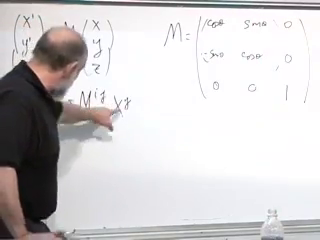
\includegraphics[width=0.82\textwidth]{lecture_05_figure_03.png}\caption{La rotation spatiale écrite à la fois sous forme d’équation matricielle et en notation indicielle.}\lectureframe{01:00:40}\end{figure}

\section{Matrices de Lorentz et composition des vitesses}

Pour un mouvement selon \(x\), la transformation de Lorentz en unités \(c=1\) s’écrit
\begin{align}
x'&=\gamma_v(x-vt), & y'&=y,\nonumber\\
z'&=z, & t'&=\gamma_v(t-vx),
\end{align}
où
\begin{equation}
\gamma_v=\frac{1}{\sqrt{1-v^2}}.
\end{equation}
Avec l’ordre des composantes \((x,y,z,t)\), elle devient
\begin{equation}
\begin{pmatrix}x'\\y'\\z'\\t'\end{pmatrix}
=
\begin{pmatrix}
\gamma_v&0&0&-\gamma_vv\\
0&1&0&0\\
0&0&1&0\\
-\gamma_vv&0&0&\gamma_v
\end{pmatrix}
\begin{pmatrix}x\\y\\z\\t\end{pmatrix}.
\label{eq:l5-lorentz-matrix}
\end{equation}

\begin{figure}[H]\centering
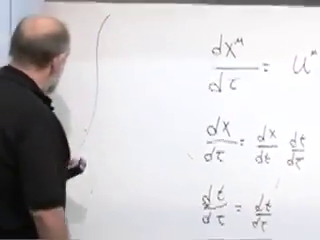
\includegraphics[width=0.82\textwidth]{lecture_05_figure_04.png}\caption{La matrice de Lorentz \(4\times4\). Seules les composantes \(x\) et \(t\) se mélangent ; \(y\) et \(z\) restent inchangées.}\lectureframe{01:04:40}\end{figure}

La multiplication matricielle permet maintenant de répondre à une question physique. Supposons qu’un observateur se déplace à la vitesse \(v\) par rapport à nous, et qu’un troisième se déplace à la vitesse \(u\) par rapport à cet observateur, tous le long du même axe. La cinématique newtonienne donnerait \(w=u+v\), ce qui permettrait de combiner deux vitesses de \(3c/4\) pour obtenir \(3c/2\). La relativité doit donner une autre règle.

La partie active du boost est la matrice \(2\times2\)
\begin{equation}
B(v)=\gamma_v
\begin{pmatrix}1&-v\\-v&1\end{pmatrix}.
\end{equation}
La composition des deux boosts donne
\begin{align}
B(u)B(v)
&=\gamma_u\gamma_v
\begin{pmatrix}1&-u\\-u&1\end{pmatrix}
\begin{pmatrix}1&-v\\-v&1\end{pmatrix}\nonumber\\
&=\gamma_u\gamma_v
\begin{pmatrix}
1+uv&-(u+v)\\
-(u+v)&1+uv
\end{pmatrix}.
\label{eq:l5-composed-boost}
\end{align}
Le rapport d’un élément hors diagonale à un élément diagonal détermine la vitesse du boost résultant :
\begin{equation}
w=\frac{u+v}{1+uv}
\qquad(c=1).
\end{equation}
En rétablissant les dimensions,
\begin{equation}
w=\frac{u+v}{1+uv/c^2}.
\label{eq:l5-velocity-addition}
\end{equation}

\begin{figure}[H]\centering
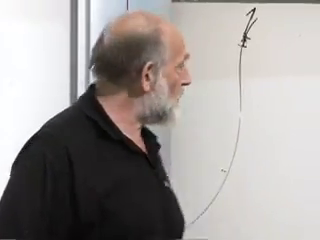
\includegraphics[width=0.82\textwidth]{lecture_05_figure_05.png}\caption{Matrice résultant de la composition de deux boosts et vitesse \(w=(u+v)/(1+uv)\) en unités naturelles.}\lectureframe{01:15:35}\end{figure}

Si \(u\) et \(v\) sont chacune proches de \(c\), le numérateur tend vers \(2c\), tandis que le dénominateur tend vers \(2\) ; ainsi, \(w\) tend vers \(c\), et non vers \(2c\). Plus généralement, l’équation~\eqref{eq:l5-velocity-addition} transforme des vitesses d’entrée inférieures à celle de la lumière en une vitesse résultante qui lui est également inférieure. La multiplication matricielle encode automatiquement la limite de vitesse.

\section{Quadrivecteurs et échec de la vitesse ordinaire}

Un quadrivecteur est un objet quelconque dont les quatre composantes se transforment sous les rotations et les boosts de Lorentz de la même manière que les coordonnées de l’espace-temps. Si \(V^\mu\) est un quadrivecteur, alors, avec notre convention de signe,
\begin{equation}
V_\mu=(-V^1,-V^2,-V^3,V^0),
\end{equation}
et sa norme invariante vaut
\begin{equation}
V_\mu V^\mu=(V^0)^2-(V^1)^2-(V^2)^2-(V^3)^2.
\end{equation}
Pour deux quadrivecteurs \(V^\mu\) et \(W^\mu\), la contraction
\begin{equation}
W_\mu V^\mu
=W^0V^0-W^1V^1-W^2V^2-W^3V^3
\end{equation}
est également invariante. Les composantes changent d’un référentiel à l’autre ; la contraction, elle, ne change pas.

La vitesse ordinaire n’a que trois composantes,
\begin{equation}
\mathbf v=\left(\frac{dx}{dt},\frac{dy}{dt},\frac{dz}{dt}\right).
\end{equation}
Lui ajouter \(dt/dt=1\) ne donne pas un quadrivecteur utile. La quatrième composante serait triviale, et l’objet ainsi obtenu ne se transformerait pas linéairement sous les transformations de Lorentz. Le temps coordonnée \(t\) change d’un référentiel à l’autre ; dériver par rapport à \(t\) compromet donc la loi de transformation recherchée.

Le temps propre apporte la solution. Le long d’une ligne d’univers, définissons
\begin{equation}
u^\mu=\frac{dX^\mu}{d\tau}.
\label{eq:l5-four-velocity}
\end{equation}
Le différentiel \(dX^\mu\) est un quadrivecteur et \(d\tau\) est invariant ; leur rapport est donc un quadrivecteur. L’adjectif ``propre'' renvoie à l’horloge au dénominateur.

La règle de dérivation en chaîne relie cet objet à la vitesse ordinaire :
\begin{equation}
\frac{dx}{d\tau}=\frac{dx}{dt}\frac{dt}{d\tau},
\end{equation}
et de même pour \(y\) et \(z\). D’après l’équation~\eqref{eq:l5-proper-time},
\begin{align}
\left(\frac{d\tau}{dt}\right)^2
&=1-\left(\frac{dx}{dt}\right)^2
    -\left(\frac{dy}{dt}\right)^2
    -\left(\frac{dz}{dt}\right)^2\nonumber\\
&=1-v^2
\qquad(c=1),
\end{align}
et par conséquent
\begin{equation}
\frac{dt}{d\tau}=\gamma_v=\frac{1}{\sqrt{1-v^2}}.
\end{equation}
Les quatre composantes sont
\begin{equation}
u^i=\gamma_v v^i,
\qquad
u^0=\gamma_v
\qquad(c=1).
\label{eq:l5-four-velocity-components}
\end{equation}
À faible vitesse, \(u^i\simeq v^i\) et \(u^0\simeq1\). À l’approche de la vitesse de la lumière, \(\gamma_v\) croît sans borne et la vitesse propre diffère fortement de la vitesse ordinaire.

\begin{figure}[H]\centering
\includegraphics[width=0.82\textwidth]{lecture_05_figure_06.png}\caption{Les quatre composantes de la vitesse propre exprimées en fonction de la vitesse ordinaire et du facteur de Lorentz.}\lectureframe{01:34:40}\end{figure}

En rétablissant les unités usuelles et en utilisant \(X^0=ct\), on obtient la forme standard
\begin{equation}
U^\mu=(\gamma_v\mathbf v,\gamma_v c)
\end{equation}
dans l’ordre spatial d’abord adopté ici. Sa norme invariante est
\begin{equation}
U_\mu U^\mu=c^2.
\end{equation}
Toute particule massive a donc une quadrivitesse de même norme invariante, bien que sa vitesse spatiale dépende du référentiel.

\section{La tangente à une ligne d’univers}

L’équation~\eqref{eq:l5-four-velocity} a un analogue euclidien familier. Le long d’une courbe dans l’espace ordinaire à trois dimensions,
\begin{equation}
ds^2=dx^2+dy^2+dz^2.
\end{equation}
Le déplacement différentiel \((dx,dy,dz)\) pointe dans la direction de la courbe, mais ce n’est pas un vecteur unitaire. En le divisant par la longueur d’arc, on obtient
\begin{equation}
\mathbf T=
\left(\frac{dx}{ds},\frac{dy}{ds},\frac{dz}{ds}\right),
\qquad
\mathbf T\cdot\mathbf T=1.
\end{equation}
La construction relativiste repose sur la même idée, en remplaçant la longueur d’arc euclidienne par le temps propre. Le vecteur \(u^\mu=dX^\mu/d\tau\) est tangent à la ligne d’univers.

\begin{figure}[H]\centering
\includegraphics[width=0.82\textwidth]{lecture_05_figure_07.png}\caption{Construction du vecteur tangent euclidien : diviser le déplacement différentiel par l’élément de longueur d’arc \(ds\). Le temps propre joue un rôle analogue le long d’une ligne d’univers de genre temps.}\lectureframe{01:39:30}\end{figure}

\begin{classroomqa}\audiencequestion{Si \(c=1\), le temps propre et la distance propre sont-ils identiques ?}\lecturerresponse{Poser \(c=1\) met le temps et la distance dans les mêmes unités ; cela n’efface pas les signes moins de la géométrie de l’espace-temps. Dans l’analogie euclidienne, \(s\) est la distance ordinaire mesurée le long d’une courbe spatiale. Le long d’une ligne d’univers de genre temps, \(\tau\) est le temps écoulé mesuré par une horloge. Les constructions sont analogues, mais les géométries sont différentes.}\end{classroomqa}

Une dérivation supplémentaire définit l’accélération propre,
\begin{equation}
a^\mu=\frac{du^\mu}{d\tau}.
\end{equation}
C’est cette grandeur qui doit remplacer \(d^2\mathbf x/dt^2\) lorsque l’on relativise la deuxième loi de Newton. Comme \(u_\mu u^\mu\) est constant,
\begin{equation}
\frac{d}{d\tau}(u_\mu u^\mu)=2u_\mu a^\mu=0,
\end{equation}
l’accélération à quatre dimensions est donc orthogonale, au sens de Minkowski, à la vitesse à quatre dimensions.\editorialnote{Cette orthogonalité découle immédiatement de la norme invariante ; elle est donnée comme conséquence mathématique suivante de la définition.}

\section{Quadrimpulsion et énergie}

La quantité de mouvement est notre dernier exemple, car elle se conserve dans les collisions et les désintégrations. La particule possède une masse intrinsèque fixe \(m\), souvent appelée masse au repos. Elle ne varie pas avec la vitesse. La quantité de mouvement relativiste est le produit de cette masse fixe par la quadrivitesse :
\begin{equation}
p^\mu=mu^\mu.
\label{eq:l5-four-momentum}
\end{equation}
En unités \(c=1\),
\begin{equation}
p^i=\gamma_v m v^i,
\qquad
p^0=\gamma_v m.
\end{equation}
À faible vitesse, \(\gamma_v\simeq1\), et les composantes spatiales se réduisent donc à la quantité de mouvement newtonienne \(m\mathbf v\). À haute vitesse, elles croissent plus rapidement que \(m\mathbf v\).

La composante temporelle est l’énergie. Avec les unités usuelles et \(X^0=ct\),
\begin{equation}
P^\mu=(\mathbf p,E/c)
=(\gamma_v m\mathbf v,\gamma_v mc),
\end{equation}
et donc
\begin{equation}
E=\gamma_v mc^2
=mc^2\left(1-\frac{v^2}{c^2}\right)^{-1/2}.
\label{eq:l5-relativistic-energy}
\end{equation}

Pour retrouver la mécanique ordinaire, posons
\(\epsilon=v^2/c^2\ll1\). Le développement binomial donne
\begin{equation}
(1-\epsilon)^p=1-p\epsilon+O(\epsilon^2).
\end{equation}
En prenant \(p=-1/2\),
\begin{align}
E
&=mc^2\left(1-\frac{v^2}{c^2}\right)^{-1/2}\nonumber\\
&=mc^2\left[1+\frac12\frac{v^2}{c^2}
  +O\!\left(\frac{v^4}{c^4}\right)\right]\nonumber\\
&=mc^2+\frac12mv^2+O\!\left(\frac{mv^4}{c^2}\right).
\label{eq:l5-energy-expansion}
\end{align}

\begin{figure}[H]\centering
\includegraphics[width=0.82\textwidth]{lecture_05_figure_08.png}\caption{Développement de l’énergie relativiste aux faibles vitesses, qui fait apparaître l’énergie au repos et l’énergie cinétique newtonienne.}\lectureframe{01:51:30}\end{figure}

Le premier terme, \(mc^2\), est présent même au repos. Dans un problème newtonien portant sur un ensemble fixe de particules dont les masses ne changent pas, ce terme apporte la même constante avant et après le mouvement ; seul \(\tfrac12mv^2\) intervient donc dans les bilans familiers. La relativité révèle que cette constante écartée était en réalité une énergie physique depuis le début.

L’énergie et la quantité de mouvement ne sont donc pas des lois de conservation sans rapport entre elles. Elles sont les quatre composantes d’un même vecteur conservé. Un boost de Lorentz les mélange : ce qu’un observateur appelle énergie contribue en partie à la quantité de mouvement d’un autre observateur, et réciproquement. Néanmoins, pour un système isolé, la quadrimpulsion totale est la même avant et après toute collision ou désintégration, dans tous les référentiels inertiels.

Nous voici au seuil de la mécanique relativiste. Les étapes suivantes consistent à exprimer la force au moyen de l’accélération propre et à comprendre les équations d’onde relativistes, en particulier celles qui régissent l’électromagnétisme et la lumière.
\chapter{Lois invariantes, quadrivecteurs et tenseur de champ}

Nous commencerons par une loi que la nature aurait pu respecter, mais qu’elle ne respecte pas. Son échec nous indiquera comment une loi physique doit être écrite. Le même critère conduit d’abord des composantes de coordonnées aux vecteurs ordinaires, puis des vecteurs ordinaires aux quadrivecteurs, et enfin des quadrivecteurs aux tenseurs. À la fin, les champs électrique et magnétique ne seront plus des objets séparés : ensemble, ils occuperont les six composantes indépendantes d’un même tenseur antisymétrique.

Sauf indication contraire, nous utilisons des unités telles que \(c=1\), ordonnons les composantes de l’espace-temps selon \((1,2,3,0)=(x,y,z,t)\) et adoptons la signature métrique \((-,-,-,+)\).

\section{Une loi possible, mais dotée d’une mauvaise symétrie}

Fixons définitivement dans l’espace un axe \(x\) et un axe \(y\). Décidons maintenant que deux particules interagissent dès que leurs coordonnées \(x\) coïncident. L’interaction pourrait inverser leur mouvement ou les envoyer dans de nouvelles directions ; sa dynamique détaillée importe peu. Le déclencheur proposé est simplement \begin{equation}
  x_1-x_2=0,
\end{equation} où les indices désignent les particules, et non les composantes de coordonnées. Cette règle ne présente aucune contradiction mathématique. La question est de savoir ce qui la rend physiquement peu plausible.

\begin{classroomqa}\audiencequestion{La règle viole-t-elle l’homogénéité de l’espace ?}\lecturerresponse{Non. Une translation de l’origine modifie les deux coordonnées de la même quantité et laisse \(x_1-x_2\) inchangé. La règle ne désigne aucun lieu privilégié. Son défaut tient à l’isotropie : elle privilégie une direction.}\end{classroomqa}

Faisons tourner les axes de \(90^\circ\). L’ancienne direction \(x\) s’appelle désormais \(y\) ; les mêmes événements physiques seraient donc décrits par l’égalité des coordonnées \(y\). Pour un angle quelconque, la condition ferait intervenir une combinaison linéaire de \(x\) et de \(y\). La forme de la loi dépend donc de l’orientation du tableau. Elle est invariante par translation, mais pas par rotation.

Nous donnons généralement aux lois physiques leur forme la plus simple dans des coordonnées orthogonales. On peut utiliser des coordonnées plus générales, mais la métrique et les formules deviennent alors moins simples. Au sein de la classe des repères cartésiens orthogonaux, aucune orientation ne doit être privilégiée.

La correction est immédiate. En deux dimensions, exigeons que les deux coordonnées coïncident ; en trois dimensions, exigeons que les trois coïncident : \begin{equation}
  x_1=x_2,
  \qquad y_1=y_2,
  \qquad z_1=z_2.
\end{equation} Les particules ne peuvent alors interagir que lorsqu’elles atteignent le même point, même si elles s’en approchent selon des lignes différentes.

\begin{classroomqa}\audiencequestion{Les coordonnées \(z\) et les temps doivent-ils aussi coïncider ?}\lecturerresponse{Dans l’espace à trois dimensions, les coordonnées \(z\) doivent également coïncider. Pour le moment, nous laissons le temps de côté ; nous le réintroduirons dès que l’argument spatial sera terminé.}\end{classroomqa}

Soit \(\boldsymbol r_a\) la position de la particule \(a\). Les trois conditions sur les composantes se ramènent à une équation vectorielle : \begin{equation}
  \boldsymbol r_1-\boldsymbol r_2=\boldsymbol 0.
\end{equation} Une composante peut s’annuler dans un repère tourné et ne pas s’annuler dans un autre. Le vecteur entier est différent : si toutes ses composantes sont nulles dans un repère, elles le sont dans tous les repères obtenus par rotation. De même, si deux vecteurs sont égaux dans un repère, ils le restent après transformation des deux vecteurs.

\begin{figure}[H]\centering
\includegraphics[width=0.78\textwidth]{lecture_06_figure_01.png}\caption{Les trois égalités de coordonnées qui font de la collision une coïncidence spatiale plutôt qu’une coïncidence le long d’un axe privilégié.}\lectureframe{00:09:00}\end{figure}

Voilà pourquoi les équations vectorielles sont utiles. Leurs composantes changent, mais l’objet se transforme de façon cohérente. Une loi écrite pour l’objet entier peut conserver sa forme lorsque les coordonnées subissent une rotation.

\section{Coïncidence dans l’espace-temps}

Remplaçons maintenant l’axe spatial vertical par le temps. Une règle newtonienne pourrait stipuler que deux changements de mouvement ne se produisent qu’à des instants égaux. En mécanique newtonienne, la simultanéité est la même pour tous les observateurs inertiels ; une telle règle est donc possible. En relativité restreinte, elle sélectionne un référentiel privilégié. Des événements simultanés dans un référentiel ne le sont pas nécessairement dans un autre.

Exiger seulement l’égalité des coordonnées spatiales ne convient pas davantage. Un déplacement dans l’espace-temps peut avoir des composantes spatiales nulles et une composante temporelle non nulle : \begin{equation}
  \Delta X^\mu=(0,0,0,\Delta t),
\end{equation} et un boost mélange \(\Delta t\) avec une composante spatiale. L’énoncé local invariant est que les deux changements de mouvement se produisent au même événement. Ainsi, une collision simple exige \begin{equation}
  X_1^\mu=X_2^\mu,
  \qquad\text{or}\qquad
  X_1^\mu-X_2^\mu=0.
\end{equation} Les quatre coordonnées coïncident : les particules occupent le même lieu au même instant.

L’exemple de la collision fournit une règle générale pour écrire la physique. Nous pouvons tout placer d’un côté et égaler un quadrivecteur complet à zéro, ou égaler un quadrivecteur complet à un autre. Égaler des composantes isolées d’un quadrivecteur ne donne pas, à lui seul, un énoncé invariant de Lorentz.

\section{Boosts, rotations et notation matricielle}

Un quadrivecteur est un objet qui se transforme comme un déplacement dans l’espace-temps. Pour rendre cette définition utile, rappelons d’abord les transformations des coordonnées elles-mêmes. Pour un boost de vitesse \(v\) dans la direction \(x\), \begin{align}
  x'&=\gamma(x-vt), & y'&=y, & z'&=z,
  & t'&=\gamma(t-vx),                                      \label{eq:l6-boost}
\end{align} où \begin{equation}
  \gamma(v)=\frac{1}{\sqrt{1-v^2}}.
\end{equation}

\begin{classroomqa}\audiencequestion{La vitesse de la lumière a-t-elle été posée égale à un dans ces formules ?}\lecturerresponse{Oui. Pour rétablir les unités, prenons \(X^0=ct\), remplaçons \(1-v^2\) par \(1-v^2/c^2\) et réintroduisons les facteurs correspondants de \(c\) dans les termes mêlant espace--temps.}\end{classroomqa}

Une rotation autour de l’axe \(z\) mélange \(x\) et \(y\), tout en laissant \(z\) et \(t\) inchangés : \begin{equation}
\begin{pmatrix}
  x'\\ y'\\ z'\\ t'
\end{pmatrix}
=
\begin{pmatrix}
  \cos\theta & \sin\theta & 0 & 0\\
  -\sin\theta & \cos\theta & 0 & 0\\
  0 & 0 & 1 & 0\\
  0 & 0 & 0 & 1
\end{pmatrix}
\begin{pmatrix}
  x\\ y\\ z\\ t
\end{pmatrix}.
\end{equation} Il vaut la peine d’afficher les zéros : ils indiquent explicitement quelles composantes n’interviennent pas dans la coordonnée transformée considérée. Dans le même ordre, le boost de l’équation~\eqref{eq:l6-boost} s’écrit \begin{equation}
\begin{pmatrix}
  x'\\ y'\\ z'\\ t'
\end{pmatrix}
=
\begin{pmatrix}
  \gamma & 0 & 0 & -\gamma v\\
  0 & 1 & 0 & 0\\
  0 & 0 & 1 & 0\\
  -\gamma v & 0 & 0 & \gamma
\end{pmatrix}
\begin{pmatrix}
  x\\ y\\ z\\ t
\end{pmatrix}.
\end{equation}

On peut composer rotations et boosts par multiplication matricielle. Pour effectuer un boost dans une direction qui n’est pas alignée sur l’axe \(x\) initial, on peut d’abord faire tourner cette direction jusqu’à l’axe \(x\), appliquer le boost, puis effectuer les rotations nécessaires. Les produits de ces matrices élémentaires engendrent des transformations de Lorentz plus générales.

\begin{classroomqa}\audiencequestion{L’ordre importe-t-il : faut-il d’abord faire une rotation puis un boost, ou d’abord un boost puis une rotation ?}\lecturerresponse{Oui. Après la première opération, les axes sur lesquels agit la seconde ont changé. Les deux produits matriciels ne sont pas nécessairement égaux ; l’ordre des opérations importe donc.}\end{classroomqa}

On peut écrire toutes ces transformations linéaires en une seule fois : \begin{equation}
  X'^{\mu}=\Lambda^{\mu}{}_{\nu}X^{\nu}.                  \label{eq:l6-vector-transform}
\end{equation} L’indice répété \(\nu\) est sommé sur \(1,2,3,0\). Il s’agit simplement de la somme habituelle, ligne par colonne, de la multiplication matricielle, exprimée en notation indicielle.

\begin{figure}[H]\centering
\includegraphics[width=0.78\textwidth]{lecture_06_figure_02.png}\caption{La transformation de Lorentz indicielle, au-dessus de son expression sous forme de vecteurs colonnes.}\lectureframe{00:31:55}\end{figure}

L’équation~\eqref{eq:l6-vector-transform} est aussi la définition d’un quadrivecteur contravariant général. Si \(A^\mu\) est un tel vecteur, alors \begin{equation}
  A'^{\mu}=\Lambda^{\mu}{}_{\nu}A^{\nu}.
\end{equation} Ses quatre composantes ne représentent pas nécessairement une position. C’est sa loi de transformation qui fait de cet objet un quadrivecteur.

\section{Scalaires, métrique et produits invariants}

Avant d’utiliser d’autres quadrivecteurs, il est utile de revenir à la notion plus simple de scalaire. Sous les rotations spatiales, la température en un point donné est un scalaire, tout comme la distance entre deux points donnés. Chacun est un nombre unique, indépendant de l’orientation des axes. On pourrait même avancer l’affirmation numérique volontairement absurde qu’une distance mesurée en centimètres est égale à la température ambiante mesurée en degrés Fahrenheit. Cette affirmation n’a aucune portée physique profonde, mais puisque ses deux membres sont des scalaires sous les rotations, sa vérité ou sa fausseté ne dépend pas de la rotation des axes.

Les composantes d’un vecteur ne sont pas des scalaires. Il nous faut donc une méthode systématique pour les combiner en scalaires. Écrivons un quadrivecteur contravariant général sous la forme \begin{equation}
  A^\mu=(A^1,A^2,A^3,A^0).
\end{equation} Les composantes covariantes décrivent le même objet géométrique avec un indice inférieur. Avec notre signature, on les obtient au moyen de la métrique de Minkowski : \begin{equation}
  A_\mu=\eta_{\mu\nu}A^\nu,
  \qquad
  \eta_{\mu\nu}=
  \begin{pmatrix}
    -1&0&0&0\\
    0&-1&0&0\\
    0&0&-1&0\\
    0&0&0&1
  \end{pmatrix},                                          \label{eq:l6-metric}
\end{equation} de sorte que \begin{equation}
  A_\mu=(-A^1,-A^2,-A^3,A^0).
\end{equation}

\begin{classroomqa}\audiencequestion{Y a-t-il deux indices et des signes incohérents au tableau ?}\lecturerresponse{Oui. Il faut ajouter le signe moins correspondant à la composante spatiale de la colonne affichée, et les composantes à droite de l’équation d’abaissement d’indice portent des indices supérieurs avant la multiplication par \(\eta_{\mu\nu}\). L’indice temporel est \(0\), et non \(4\).}\end{classroomqa}

\begin{figure}[H]\centering
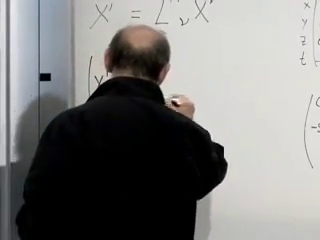
\includegraphics[width=0.8\textwidth]{lecture_06_figure_03.png}\caption{Composantes contravariantes et covariantes, matrice métrique et début de la contraction invariante.}\lectureframe{00:45:00}\end{figure}

L’abaissement d’indice n’est pas une simple convention décorative. Il incorpore les signes nécessaires à la norme invariante de Lorentz : \begin{align}
  A_\mu A^\mu
  &=-(A^1)^2-(A^2)^2-(A^3)^2+(A^0)^2,                    \label{eq:l6-norm}\\
  X_\mu X^\mu
  &=t^2-x^2-y^2-z^2.
\end{align} La seconde expression est l’intervalle d’espace-temps invariant mesuré depuis l’origine. Comme \(A^\mu\) se transforme de la même façon que \(X^\mu\), leur contraction conserve elle aussi son invariance.

La notation nous enseigne également une règle pratique de calcul. Un indice de sommation répété apparaît une fois en position supérieure et une fois en position inférieure. Par exemple, \begin{equation}
  A_\mu A^\mu
  =\eta_{\mu\nu}A^\mu A^\nu.
\end{equation} On peut changer le nom des indices sommés, ou indices muets, sans modifier la quantité.

\begin{classroomqa}\audiencequestion{Faut-il considérer l’un de ces vecteurs comme une ligne et l’autre comme une colonne, et leur ordre importe-t-il ?}\lecturerresponse{Pour le calcul présent, considérons les quantités indicées comme des composantes et laissons la métrique effectuer la contraction ; inutile de ramener la discussion à l’algèbre des opérateurs en lignes et en colonnes. Ce sont des nombres ordinaires, donc leur ordre importe peu. Les opérateurs qui ne commutent pas exigeraient davantage de précautions, mais ce n’est pas le sujet ici.}\end{classroomqa}

La même construction définit un produit scalaire entre deux quadrivecteurs distincts : \begin{equation}
  A\mathbin{\cdot}B=A_\mu B^\mu=A^\mu B_\mu.
\end{equation} Son invariance se démontre sans écrire explicitement une matrice de Lorentz. Puisque \(A+B\) et \(A-B\) sont des quadrivecteurs, leurs normes au carré sont invariantes : \begin{align}
  (A+B)^2&=A^2+B^2+2A\mathbin{\cdot}B,\\
  (A-B)^2&=A^2+B^2-2A\mathbin{\cdot}B.
\end{align} En faisant la différence, on obtient \begin{equation}
  (A+B)^2-(A-B)^2=4A\mathbin{\cdot}B,                    \label{eq:l6-polarization}
\end{equation} ; ainsi \(A\mathbin{\cdot}B\) est également invariant. Le facteur quatre découle directement du développement.\editorialnote{L’argument au tableau donne cette identité de polarisation ; écrire explicitement le facteur lève toute ambiguïté sur la simplification évoquée à l’oral.}

\begin{figure}[H]\centering
\includegraphics[width=0.8\textwidth]{lecture_06_figure_04.png}\caption{Les deux carrés invariants utilisés pour isoler le produit scalaire de quadrivecteurs distincts.}\lectureframe{00:52:20}\end{figure}

Les quantités invariantes sont des ingrédients naturels des lois physiques : contrairement à une composante isolée, elles conservent la même valeur d’un référentiel à l’autre.

\section{Vitesse propre et quadrivecteur énergie-impulsion}

Considérons deux événements voisins sur la ligne d’univers d’une particule. Leur séparation est le quadrivecteur infinitésimal \begin{equation}
  dX^\mu=(dx,dy,dz,dt).
\end{equation} Pour une ligne d’univers de genre temps, le temps propre est défini par \begin{equation}
  d\tau^2=dX_\mu dX^\mu
  =dt^2-dx^2-dy^2-dz^2.                                  \label{eq:l6-proper-time}
\end{equation} Le quadrivecteur vitesse propre est \begin{equation}
  U^\mu=\frac{dX^\mu}{d\tau}.                            \label{eq:l6-four-velocity}
\end{equation} Il mesure le taux de variation de la position dans l’espace-temps par rapport au temps propre de la particule, et non par rapport au temps coordonné d’un référentiel choisi.

Bien que \(U^\mu\) ait quatre composantes, seules trois sont indépendantes. En divisant l’équation~\eqref{eq:l6-proper-time} par \(d\tau^2\), on obtient \begin{equation}
  U_\mu U^\mu=1.
\end{equation} Le quadrivecteur vitesse propre est donc un vecteur unitaire de genre temps. Le choix orienté vers le futur fixe le signe de sa composante temporelle.

\begin{classroomqa}
\audiencequestion{À des vitesses très inférieures à \(c\), la quadrivitesse se réduit-elle à la vitesse ordinaire ?}
\lecturerresponse{Ses trois composantes spatiales tendent vers la vitesse ordinaire, tandis que sa composante temporelle tend vers l’unité dans les unités \(c=1\). Cette relation découle de l’application de la règle de la chaîne et du calcul de \(dt/d\tau\).}
\end{classroomqa}

Pour chaque composante spatiale, \begin{equation}
  U^i=\frac{dx^i}{d\tau}
     =\frac{dx^i}{dt}\frac{dt}{d\tau}
     =v^i\frac{dt}{d\tau}.
\end{equation} Divisons l’équation~\eqref{eq:l6-proper-time} par \(dt^2\) : \begin{equation}
  \left(\frac{d\tau}{dt}\right)^2
  =1-v_x^2-v_y^2-v_z^2
  =1-\boldsymbol v^2.
\end{equation} On en déduit \begin{equation}
  \frac{dt}{d\tau}=\frac{1}{\sqrt{1-\boldsymbol v^2}}
  =\gamma(\lvert\boldsymbol v\rvert),
\end{equation} et \begin{equation}
  U^\mu=(\gamma v_x,\gamma v_y,\gamma v_z,\gamma).
                                                                  \label{eq:l6-u-components}
\end{equation}

\begin{figure}[H]\centering
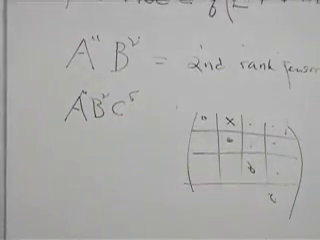
\includegraphics[width=0.8\textwidth]{lecture_06_figure_05.png}\caption{Le calcul du temps propre qui donne \(dt/d\tau=\gamma\) et relie la vitesse propre à la vitesse ordinaire.}\lectureframe{01:02:00}\end{figure}

\begin{classroomqa}\audiencequestion{\(dx^2/dt^2\) désigne-t-il une dérivée seconde, et le carré d’un vecteur doit-il produire des termes croisés ?}\lecturerresponse{Ici, il désigne \((dx/dt)^2\), le carré d’une dérivée première. De plus, \(\boldsymbol v^2\) désigne le produit scalaire euclidien \(v_x^2+v_y^2+v_z^2\), et non le carré de la somme formelle \(v_x+v_y+v_z\) ; il n’y a pas de termes croisés.}\end{classroomqa}

\begin{classroomqa}\audiencequestion{\(v\) dans \(\gamma(v)\) désigne-t-il la vitesse relative de deux référentiels ou la vitesse de la particule ?}\lecturerresponse{Ici, il s’agit de la vitesse de la particule dans le référentiel choisi. La fonction \(\gamma(v)=1/\sqrt{1-v^2}\) peut être évaluée pour n’importe quelle vitesse : dans un boost, on l’évalue à la vitesse relative des référentiels ; dans le quadrivecteur vitesse propre, on l’évalue à la vitesse de la particule.}\end{classroomqa}

Pour \(v\ll1\), \(\gamma\simeq1\), de sorte que les composantes spatiales de \(U^\mu\) tendent vers \(\boldsymbol v\) et que \(U^0\) tend vers un. Lorsque la vitesse ordinaire tend vers la vitesse de la lumière, \(\gamma\) et toutes les composantes non nulles du quadrivecteur vitesse propre croissent sans borne.

\begin{classroomqa}\audiencequestion{\(U^0\) ne devrait-il pas avoir les unités d’une vitesse plutôt que d’être proche du nombre un ?}\lecturerresponse{Les unités ont disparu lorsque \(c\) a été posé égal à un. Avec \(X^0=ct\), on a \(U^\mu=(\gamma\boldsymbol v,\gamma c)\), de sorte que la composante temporelle tend vers \(c\) et \(U_\mu U^\mu=c^2\).}\end{classroomqa}

Pour une particule de masse au repos \(m\), définissons le quadrivecteur énergie-impulsion par \begin{equation}
  P^\mu=mU^\mu.
\end{equation} En unités naturelles, \begin{equation}
  P^\mu=(\gamma m\boldsymbol v,\gamma m).
\end{equation} À faible vitesse, les trois premières composantes tendent vers la quantité de mouvement newtonienne \(m\boldsymbol v\). Le rétablissement des unités donne \begin{equation}
  P^\mu=(\gamma m\boldsymbol v,E/c),
  \qquad E=\gamma mc^2,
\end{equation} et donc \begin{equation}
  E=mc^2+\frac{1}{2}m\boldsymbol v^2+O(mv^4/c^2).
\end{equation} La composante temporelle est l’énergie en unités \(c=1\), ou l’énergie divisée par \(c\) si l’on attribue à toutes les composantes les unités d’une quantité de mouvement.

\begin{classroomqa}\audiencequestion{La vitesse ordinaire \(\boldsymbol v\), à laquelle on ajoute une quatrième composante, constitue-t-elle elle-même un quadrivecteur ?}\lecturerresponse{Non. La vitesse ordinaire à trois composantes ne se transforme pas comme un quadrivecteur. Le facteur \(\gamma\) et la définition par le temps propre sont essentiels ; le quadrivecteur est \(U^\mu\), et non \(\boldsymbol v\).}\end{classroomqa}

\section{Pourquoi les champs électrique et magnétique doivent se mélanger}

Nous allons maintenant faire une brève parenthèse loin de la relativité. Partons de l’équation du mouvement d’avant Einstein et demandons-nous comment la réorganiser pour qu’elle soit valable dans tous les référentiels inertiels. L’accélération ordinaire est la dérivée temporelle de la vitesse ordinaire. Son analogue quadridimensionnel est naturellement \begin{equation}
  A^\mu=\frac{dU^\mu}{d\tau}.
\end{equation} À faible vitesse, ses composantes spatiales tendent vers l’accélération ordinaire. Nous reporterons l’équation relativiste complète ; examinons d’abord l’ancienne loi de force.

Pour une charge \(q\) dans des champs électrique et magnétique, \begin{equation}
  \boldsymbol F=m\boldsymbol a
  =q\left(\boldsymbol E+\boldsymbol v\times\boldsymbol B\right).
                                                                  \label{eq:l6-lorentz-force}
\end{equation} Le terme électrique ne dépend pas de la vitesse de la particule, contrairement au terme magnétique.

\begin{figure}[H]\centering
\includegraphics[width=0.8\textwidth]{lecture_06_figure_06.png}\caption{La forme prérelativiste de la force de Lorentz, qui motive la réunion de \(\boldsymbol E\) et \(\boldsymbol B\).}\lectureframe{01:18:20}\end{figure}

Supposons qu’un observateur ne voie aucun champ électrique, mais détecte un champ magnétique et une charge en mouvement. La charge subit une force magnétique. Dans le référentiel instantanément au repos de la charge, toutefois, \(\boldsymbol v=0\) ; le terme magnétique de l’équation~\eqref{eq:l6-lorentz-force} s’annule donc. La ligne d’univers physique n’est pas devenue inertielle du seul fait que les coordonnées ont changé ; la force dans le nouveau référentiel doit donc comporter une contribution électrique. Plus précisément, une quadraccélération non nulle ne peut pas être transformée en zéro par un changement de référentiel inertiel, même si l’accélération à trois dimensions et ses composantes, elles, se transforment. \editorialnote{Cet énoncé sur la quadraccélération est la formulation invariante de l’argument présenté en cours et évite de traiter l’accélération ordinaire à trois dimensions comme si elle était invariante de référentiel.}

Les champs électrique et magnétique doivent donc se transformer l’un en l’autre. Ensemble, ils ont six composantes : ils ne forment donc ni un scalaire unique ni un quadrivecteur. Il nous faut un nouvel objet transformé.

\section{Tenseurs : une transformation pour chaque indice}

On peut appeler un scalaire un tenseur de rang zéro ; il ne porte aucun indice. Un quadrivecteur est un tenseur de rang un ; il porte un indice qui peut prendre quatre valeurs. L’exemple le plus simple de rang deux est un produit \begin{equation}
  A^\mu B^\nu.
\end{equation} Chaque indice peut prendre quatre valeurs ; l’objet possède donc \(4^2=16\) composantes, que l’on peut représenter dans un tableau \(4\times4\). Un produit de trois vecteurs, \begin{equation}
  A^\mu B^\nu C^\sigma,
\end{equation}, possède \(4^3=64\) composantes et est un tenseur de rang trois. Les rangs supérieurs suivent le même principe. Le nom importe moins que la règle qui définit l’objet.

Si \begin{equation}
  A'^{\mu}=\Lambda^\mu{}_{\nu}A^\nu,
  \qquad
  B'^{\sigma}=\Lambda^\sigma{}_{\tau}B^\tau,
\end{equation} alors leur produit se transforme selon \begin{equation}
  A'^{\mu}B'^{\sigma}
  =\Lambda^\mu{}_{\nu}\Lambda^\sigma{}_{\tau}
   A^\nu B^\tau.
\end{equation} On obtient ainsi la loi définissant un tenseur contravariant de rang deux : \begin{equation}
  T'^{\mu\sigma}
  =\Lambda^\mu{}_{\nu}\Lambda^\sigma{}_{\tau}T^{\nu\tau}.
                                                                  \label{eq:l6-tensor-transform}
\end{equation} Une matrice de Lorentz intervient pour chaque indice. Les indices répétés \(\nu\) et \(\tau\) sont sommés ; les indices libres \(\mu\) et \(\sigma\) désignent la composante calculée dans le référentiel primé.

\begin{figure}[H]\centering
\includegraphics[width=0.82\textwidth]{lecture_06_figure_07.png}\caption{La transformation de deux vecteurs et la loi de transformation à deux matrices qui en résulte pour un tenseur de rang deux.}\lectureframe{01:27:15}\end{figure}

Un tenseur n’est pas nécessairement le produit unique de vecteurs. \(A^\mu B^\nu\) et \(A^\nu B^\mu\) respectent tous deux la loi de transformation d’un tenseur, de même que leur somme et toute somme telle que \begin{equation}
  A^\mu B^\nu+C^\mu D^\nu.
\end{equation} C’est la loi de transformation, et non une factorisation particulière, qui définit le tenseur. Un tenseur de rang trois comporte une troisième matrice de Lorentz, et ainsi de suite.

\section{Tenseurs symétriques et antisymétriques}

Deux classes de tenseurs de rang deux seront particulièrement utiles. Un tenseur symétrique vérifie \begin{equation}
  T^{\mu\nu}=T^{\nu\mu},
\end{equation} ; les éléments symétriques par rapport à la diagonale sont donc égaux. Ses quatre éléments diagonaux et les six éléments situés d’un côté de la diagonale déterminent les autres, ce qui donne \begin{equation}
  4+6=10
\end{equation} composantes indépendantes.

Un tenseur antisymétrique vérifie \begin{equation}
  T^{\mu\nu}=-T^{\nu\mu}.                                \label{eq:l6-antisymmetry}
\end{equation} En posant \(\mu=\nu\) dans l’équation~\eqref{eq:l6-antisymmetry}, on obtient \(T^{\mu\mu}=-T^{\mu\mu}\) ; tous les éléments diagonaux sont donc nuls. Les six éléments d’une moitié triangulaire déterminent les six autres, avec un changement de signe. Il y a donc exactement six composantes indépendantes.

\begin{figure}[H]\centering
\includegraphics[width=0.82\textwidth]{lecture_06_figure_08.png}\caption{Un tableau antisymétrique \(4\times4\) complet : des zéros sur la diagonale et des signes opposés de part et d’autre.}\lectureframe{01:34:25}\end{figure}

Ce dénombrement fournit l’indice recherché. Les trois composantes électriques et les trois composantes magnétiques peuvent se regrouper en un tenseur antisymétrique de rang deux.

\section{Le tenseur électromagnétique}

Faisons courir les indices d’espace-temps sur les lignes et les colonnes dans l’ordre \((1,2,3,0)=(x,y,z,t)\). La disposition écrite au tableau est \begin{equation}
  F_{\mu\nu}=
  \begin{pmatrix}
    0    & -B_3 & B_2  & E_1\\
    B_3  & 0    & -B_1 & E_2\\
    -B_2 & B_1  & 0    & E_3\\
    -E_1 & -E_2 & -E_3 & 0
  \end{pmatrix}.                                         \label{eq:l6-field-tensor}
\end{equation} Les composantes purement spatiales contiennent le champ magnétique ; celles qui portent un indice spatial et un indice temporel contiennent le champ électrique. L’antisymétrie fournit les éléments du triangle inférieur une fois connus ceux du triangle supérieur.

\begin{classroomqa}\audiencequestion{Les composantes magnétiques sont-elles toutes négatives, et les indices correspondent-ils à \(x,y,z\) ?}\lecturerresponse{Dans le triangle spatial supérieur, les signes alternent comme indiqué : \(-B_3,+B_2,-B_1\). Les indices \(1,2,3\) correspondent à \(x,y,z\), tandis que \(0\) désigne le temps. La réflexion par rapport à la diagonale inverse chaque signe.}\end{classroomqa}

\begin{figure}[H]\centering
\includegraphics[width=0.82\textwidth]{lecture_06_figure_09.png}\caption{Le tenseur électromagnétique complété, dans l’ordre des composantes utilisé au cours, avec les coordonnées spatiales en premier.}\lectureframe{01:41:05}\end{figure}

La notation usuelle est \(F_{\mu\nu}\), plutôt qu’un \(T_{\mu\nu}\) générique. Le professeur avance l’hypothèse que la lettre pourrait renvoyer à Faraday, tout en précisant qu’il ne connaît pas l’histoire de cette notation. Ce qui compte ici, c’est l’antisymétrie et les six composantes du champ, et non cette hypothèse sur la lettre.

\begin{classroomqa}\audiencequestion{Chaque élément de la matrice représente-t-il l’intensité du champ dans le plan de coordonnées indiqué ?}\lecturerresponse{C’est une composante du tenseur électromagnétique. Les éléments qui font intervenir le temps sont des composantes électriques, et les éléments spatiaux--spatiaux codent les composantes magnétiques.}\end{classroomqa}

Délimitons la ligne et la colonne portant l’indice temporel. Le bloc antisymétrique restant \(3\times3\) est magnétique. On peut retenir ses composantes indépendantes selon un cycle : \begin{equation}
  F_{12}=-B_3,
  \qquad F_{23}=-B_1,
  \qquad F_{31}=-B_2.                                   \label{eq:l6-magnetic-cycle}
\end{equation} À partir de la première relation, faisons avancer chaque indice dans l’ordre \(1\to2\to3\to1\). De manière équivalente, \begin{equation}
  F_{ij}=-\epsilon_{ijk}B_k,
\end{equation} avec \(\epsilon_{123}=+1\).\editorialnote{La formule de Levi--Civita est la forme compacte usuelle de la règle cyclique explicitée au tableau.}

\begin{figure}[H]\centering
\includegraphics[width=0.82\textwidth]{lecture_06_figure_10.png}\caption{Les composantes spatiales cycliques qui codent le champ magnétique dans le tenseur antisymétrique.}\lectureframe{01:46:20}\end{figure}

Les identifications électriques sont plus directes : \begin{equation}
  E_1=F_{10},
  \qquad E_2=F_{20},
  \qquad E_3=F_{30}.
\end{equation}

Le champ magnétique admet donc deux descriptions utiles. Dans l’espace à trois dimensions, on peut associer un vecteur axial à trois composantes à un tenseur antisymétrique \(3\times3\). Dans l’espace-temps, en revanche, il n’est que la partie spatiale du tenseur à six composantes \(F_{\mu\nu}\). Cette association est propre à trois dimensions : un tenseur antisymétrique \(4\times4\) possède six composantes indépendantes et ne peut pas être identifié à un quadrivecteur. \editorialnote{Sous les rotations propres, le champ magnétique se comporte comme un vecteur ; sous les réflexions, il est plus précisément un vecteur axial, ou pseudovecteur.}

Le but de cette construction n’est pas de compter les composantes pour le seul plaisir du calcul. Puisque \(F_{\mu\nu}\) se transforme comme un tenseur, un boost de Lorentz mélange automatiquement ses composantes électriques et magnétiques. Dans le prochain cours, on pourra le combiner au quadrivecteur vitesse propre et à la quadraccélération pour remplacer l’équation~\eqref{eq:l6-lorentz-force} par une équation covariante du mouvement.

\section{Questions sur Einstein et Minkowski}

Les dernières minutes quittent le formalisme pour revenir à son origine historique. Les réponses sont présentées comme des souvenirs plutôt que comme une histoire établie ; cette réserve fait partie de l’échange.

\begin{classroomqa}\audiencequestion{Einstein recherchait-il une formulation invariante de Lorentz pour des raisons conceptuelles, ou était-il motivé par des observations particulières ?}\lecturerresponse{Le principe selon lequel les lois de la nature doivent avoir la même forme dans tous les référentiels inertiels était au cœur de son raisonnement. Il existait aussi des données expérimentales sur la lumière et sur l’échec de la détection d’un mouvement dans l’éther, mais le professeur précise qu’il ne sait pas exactement quels résultats Einstein connaissait ni dans quelle mesure ils l’ont influencé. L’exigence conceptuelle était que les équations de Maxwell et la force de Lorentz respectent le principe de relativité, ce qui impose aux champs électrique et magnétique ainsi qu’aux composantes de la vitesse de se transformer ensemble.}\end{classroomqa}

Dans son exposé de 1905, Einstein n’utilisait pas la notation compacte des quadrivecteurs employée ici. Il procédait composante par composante et écrivait explicitement les facteurs nécessaires de \(\gamma\) et de vitesse. Minkowski a ensuite organisé géométriquement cette même structure en un espace-temps à quatre dimensions.

\begin{classroomqa}\audiencequestion{Einstein s’est-il opposé à la formulation de l’espace-temps de Minkowski, et combien de temps après Minkowski l’a-t-il introduite ?}\lecturerresponse{Selon le souvenir rapporté en cours, Einstein n’a pas accueilli favorablement au départ le langage géométrique à quatre dimensions, mais en a rapidement reconnu l’intérêt. La date est donnée avec prudence comme étant environ deux ans après l’article de 1905, peut-être en 1907 ; l’intervenant souligne qu’il se souvient de cette histoire, sans prétendre l’établir.}\end{classroomqa}

\begin{classroomqa}\audiencequestion{Minkowski était-il mathématicien ou physicien, à quoi a-t-il contribué d’autre, et a-t-il été influencé par Lorentz ou FitzGerald ?}\lecturerresponse{Aucune réponse catégorique n’est avancée. La distinction entre mathématicien et physicien n’a pas été approfondie, une remarque générale sur les autres travaux de Minkowski est interrompue par une correction du public, et les éventuelles influences restent expressément incertaines. Pour cette discussion, le point établi est que Minkowski a organisé de manière décisive la relativité au moyen d’une notation géométrique à quatre dimensions.}\end{classroomqa}

\begin{classroomqa}\audiencequestion{Les transformations qui mélangent \(\boldsymbol E\) et \(\boldsymbol B\) figuraient-elles déjà dans les travaux d’Einstein de 1905 ?}\lecturerresponse{Oui, mais elles étaient écrites composante par composante plutôt que sous la forme d’une équation unique pour le tenseur de champ. La comparaison faite en cours porte sur les équations de Maxwell écrites composante par composante : le contenu peut exister avant que la notation compacte n’en révèle la structure commune. Minkowski a systématisé cette structure dans le langage de l’espace-temps.}\end{classroomqa}‌

Cela nous ramène au point mathématique par lequel nous avons commencé. Les composantes sont indispensables au calcul, mais la loi devient intelligible lorsqu’on reconnaît qu’elles font partie d’un seul objet soumis à une transformation. La tâche suivante consiste à utiliser \(F_{\mu\nu}\) pour écrire l’équation du mouvement de la particule chargée sous une forme identique dans tous les référentiels inertiels.
\chapter{Particules chargées, transformations des champs et ondes relativistes}

La dernière fois, nous avons commencé à nous demander comment se déplace une particule chargée dans des champs électrique et magnétique lorsque l’on impose les principes de la relativité. La loi de force de Lorentz familière nous en donne déjà l’indice : son terme magnétique dépend de la vitesse de la particule, si bien que des observateurs différents ne peuvent pas s’accorder séparément sur ce qui est électrique et sur ce qui est magnétique. Notre tâche consiste à formuler la loi de façon que tous les observateurs inertiels utilisent la même équation, même si les champs et la vitesse de la particule changent d’un référentiel à l’autre.

Sauf indication contraire, nous utilisons des unités dans lesquelles \(c=1\) et la signature métrique \((-,-,-,+)\). Les composantes de l’espace-temps sont ordonnées en plaçant d’abord les trois composantes spatiales :
\begin{equation}
  \mu=(1,2,3,0)=(x,y,z,t).
\end{equation}
Les indices latins \(m,n\) ne parcourent que les trois directions spatiales.

\section{Ce qui subsiste de la loi de force de Newton}

En mécanique newtonienne,
\begin{equation}
  \boldsymbol F=m\boldsymbol a
\end{equation}
a la même forme dans tous les référentiels inertiels, car les observateurs galiléens s’accordent sur l’accélération. Ils attribuent aussi à la particule la même masse et la même force. Dès lors que la cinématique change, rien ne permet de s’attendre à ce que cette relation particulière entre la force et l’accélération ordinaire demeure inchangée.

L’électromagnétisme et la gravitation nous avertissent déjà que leurs extensions relativistes n’ont pas nécessairement à se ressembler. La loi de Coulomb et la loi de la gravitation de Newton sont toutes deux des lois en inverse du carré, mais la gravitation ne peut être intégrée naturellement à la relativité restreinte sans une modification plus profonde de la géométrie de l’espace-temps. C’est possible pour l’électromagnétisme. En fait, le magnétisme est lui-même un effet relativiste : lorsque l’on réintroduit les facteurs de \(c\), une force magnétique comporte un facteur égal à la vitesse divisée par \(c\), et elle disparaît dans la limite formelle \(c\to\infty\).

La partie durable de la loi de Newton est l’affirmation selon laquelle la force est le taux de variation de la quantité de mouvement. Pour une masse au repos constante,
\begin{equation}
  \boldsymbol F
  =m\frac{d\boldsymbol v}{dt}
  =\frac{d}{dt}(m\boldsymbol v)
  =\frac{d\boldsymbol p}{dt}.
\end{equation}
La relativité modifiera la relation entre la quantité de mouvement et la vitesse, mais préservera cette façon d’organiser l’équation.

\begin{figure}[H]
\centering
\includegraphics[width=0.64\textwidth]{lecture_07_figure_01.png}
\caption{La force réécrite sous la forme \(d\boldsymbol p/dt\), tandis que la partie électrique de la loi de Lorentz est inscrite au tableau.}
\lectureframe{00:08:20}
\end{figure}

Dans les unités \(c=1\), la loi de force de Lorentz prérelativiste s’écrit
\begin{equation}
  \frac{d\boldsymbol p}{dt}
  =q\bigl(\boldsymbol E+\boldsymbol v\times\boldsymbol B\bigr).
  \label{eq:lorentz-three}
\end{equation}
Les deux champs peuvent dépendre de la position et du temps. La limite non relativiste est maintenant la limite \(v\ll 1\), et non une limite dans laquelle la constante numérique \(c=1\) changerait d’une manière ou d’une autre. Le terme électrique de \eqref{eq:lorentz-three} est déjà un vecteur ordinaire. Pour comprendre le terme magnétique sous une forme qui puisse être transposée à l’espace-temps, nous devons réexaminer le produit vectoriel.

\section{Le produit vectoriel comme tenseur antisymétrique}

Considérons deux vecteurs tridimensionnels \(\boldsymbol A\) et \(\boldsymbol B\).
Leur produit tensoriel
\begin{equation}
  T_{mn}=A_mB_n
\end{equation}
est un tenseur de rang deux à neuf composantes. En général, il n’a pas de symétrie. Son antisymétrisation donne
\begin{equation}
  K_{mn}=A_mB_n-A_nB_m,
  \qquad K_{mn}=-K_{nm}.
  \label{eq:antisym-product}
\end{equation}
Ses éléments diagonaux sont nuls, et chaque élément sous la diagonale est déterminé par l’élément correspondant au-dessus de celle-ci. Un tenseur antisymétrique \(3\times3\) ne possède donc que trois composantes indépendantes.

Ce décompte est évocateur, mais il ne suffit pas à lui seul. Trois quantités ne se transforment pas automatiquement comme un vecteur. En trois dimensions, toutefois, on peut identifier les trois éléments indépendants de \eqref{eq:antisym-product} aux composantes du produit vectoriel
\(\boldsymbol C=\boldsymbol A\times\boldsymbol B\). Au tableau, \(C_2\) est d’abord placé provisoirement dans la position supérieure droite :

\begin{figure}[H]
\centering
\includegraphics[width=0.75\textwidth]{lecture_07_figure_02.png}
\caption{Le produit antisymétrique, dont les trois éléments indépendants sont mis en correspondance avec les composantes de \(\boldsymbol C\). L’étiquette en haut à droite est encore provisoire.}
\lectureframe{00:17:33}
\end{figure}

En faisant le cycle \(1\to2\to3\to1\), on obtient les formules des composantes
\begin{align}
  C_3 &= A_1B_2-A_2B_1, \\
  C_1 &= A_2B_3-A_3B_2, \\
  C_2 &= A_3B_1-A_1B_3.
  \label{eq:cross-components}
\end{align}
La dernière ligne montre que l’élément supérieur droit est \(-C_2\), et non \(C_2\). Cette correction fait partie de l’argument ; ce n’est pas un détail à dissimuler.

\begin{figure}[H]
\centering
\includegraphics[width=0.62\textwidth]{lecture_07_figure_03.png}
\caption{Les identités cycliques complètes entre les composantes, qui déterminent le signe provisoire dans le tableau antisymétrique.}
\lectureframe{00:21:54}
\end{figure}

La matrice obtenue est
\begin{equation}
  K_{mn}=
  \begin{pmatrix}
    0 & C_3 & -C_2 \\
    -C_3 & 0 & C_1 \\
    C_2 & -C_1 & 0
  \end{pmatrix}.
  \label{eq:cross-matrix}
\end{equation}

Cette notation repose sur une géométrie utile. Une composante dont les indices sont \(1,2\) appartient naturellement au plan \(xy\) et est identifiée à une composante vectorielle selon l’axe \(z\) qui lui est perpendiculaire. On peut décrire le même objet orienté soit par un plan, soit par une flèche normale à ce plan. La description par une flèche est propre à trois dimensions ; en dimensions supérieures, un tenseur antisymétrique de rang deux existe toujours, mais il n’a plus le même nombre de composantes qu’un vecteur. C’est donc le tenseur, et non la flèche perpendiculaire, qui constitue la forme généralisable du produit vectoriel.

De manière équivalente, après avoir choisi une orientation,
\begin{equation}
  C_k=\frac12\epsilon_{kmn}K_{mn}.
\end{equation}
La nécessité de choisir une orientation est à l’origine de la règle de la main droite et de la distinction familière entre vecteurs polaires et axiaux.
\editorialnote{La formule avec le symbole de Levi--Civita et la terminologie des vecteurs axiaux sont des notations usuelles pour la géométrie qui distingue le plan de sa normale et qui est explicitée dans le cours.}

\section{Le champ magnétique sous forme tensorielle}

La même description duale s’applique au champ magnétique. Nous définissons son tenseur spatial antisymétrique par
\begin{equation}
  B_{mn}=
  \begin{pmatrix}
    0 & -B_3 & B_2 \\
    B_3 & 0 & -B_1 \\
    -B_2 & B_1 & 0
  \end{pmatrix}.
  \label{eq:magnetic-tensor}
\end{equation}
Le signe global supplémentaire par rapport à \eqref{eq:cross-matrix} relève d’une convention. Une fois celle-ci choisie, il faut l’appliquer de manière cohérente ; changer le signe des trois composantes vectorielles décrirait la même identification entre tenseur et vecteur, mais avec la convention d’orientation opposée.

\begin{figure}[H]
\centering
\includegraphics[width=0.72\textwidth]{lecture_07_figure_04.png}
\caption{Le champ magnétique représenté à la fois par un tableau spatial antisymétrique et par ses trois composantes vectorielles.}
\lectureframe{00:24:40}
\end{figure}

Considérons maintenant la troisième composante du produit vectoriel :
\begin{align}
  (\boldsymbol v\times\boldsymbol B)_3
  &=v_1B_2-v_2B_1 \\
  &=v_1B_{13}+v_2B_{23}+v_3B_{33}.
\end{align}
On peut ajouter le dernier terme parce que \(B_{33}=0\). En faisant cycler la composante libre, on obtient la règle compacte
\begin{equation}
  (\boldsymbol v\times\boldsymbol B)_m=v_nB_{nm},
  \label{eq:cross-contraction}
\end{equation}
où l’indice répété \(n\) est sommé. La force magnétique s’écrit donc
\begin{equation}
  F_m^{(B)}=qv_nB_{nm}.
\end{equation}

\begin{figure}[H]
\centering
\includegraphics[width=0.78\textwidth]{lecture_07_figure_05.png}
\caption{La troisième composante de \(\boldsymbol v\times\boldsymbol B\) et son expression générale comme contraction avec \(B_{nm}\).}
\lectureframe{00:28:30}
\end{figure}

\begin{classroomqa}\audiencequestion{L’indice libre \(m\) désigne-t-il une composante magnétique distincte de la force ?}
\lecturerresponse{Non. Il désigne la composante spatiale de la force que l’on calcule. Pour l’argument présent, le champ électrique a simplement été posé égal à zéro, et tous les indices ici ne parcourent que les trois directions spatiales.}
\end{classroomqa}

La notation tensorielle rend presque automatique la propriété selon laquelle un champ magnétique ne fournit aucun travail. Dérivons le carré de la vitesse :
\begin{align}
  \frac{d}{dt}(v_mv_m)
  &=2\dot v_m v_m \\
  &\propto 2(\boldsymbol v\times\boldsymbol B)_m v_m \\
  &=2v_nB_{nm}v_m.
  \label{eq:speed-derivative}
\end{align}
Les termes tels que \(m=n\) s’annulent, car la diagonale de \(B_{nm}\) est nulle. Chaque terme hors diagonale a un terme correspondant dans lequel \(m\) et \(n\) sont intervertis ; les deux s’annulent parce que \(v_nv_m\) est symétrique, tandis que \(B_{nm}\) est antisymétrique. On a donc
\begin{equation}
  \frac{d}{dt}(v_mv_m)=0.
\end{equation}
Une force purement magnétique dévie la trajectoire sans modifier la vitesse ni l’énergie cinétique.

\begin{figure}[H]
\centering
\includegraphics[width=0.68\textwidth]{lecture_07_figure_06.png}
\caption{Les termes associés dans \(v_nB_{nm}v_m\) s’annulent parce que le tenseur magnétique change de signe lorsque l’on intervertit ses indices.}
\lectureframe{00:35:40}
\end{figure}

Cette démonstration est volontairement plus élaborée que le simple énoncé selon lequel un produit vectoriel est perpendiculaire à son premier facteur. Cette dernière propriété est propre à la représentation vectorielle en trois dimensions. La contraction d’une paire symétrique avec un tenseur antisymétrique est l’argument qui se conservera en quatre dimensions.

\begin{classroomqa}\audiencequestion{Le champ magnétique doit-il être indépendant du temps pour que la vitesse reste constante ?}
\lecturerresponse{L’algèbre ci-dessus ne dérive jamais le champ et n’exige pas que \(\partial_t\boldsymbol B=0\). Un terme magnétique seul ne fournit toujours aucun travail. En électrodynamique, cependant, un champ magnétique variable produit un champ électrique, et ce champ électrique peut modifier la vitesse de la particule.}
\end{classroomqa}

\section{Pourquoi les champs électrique et magnétique doivent se mélanger}

Le mélange de \(\boldsymbol E\) et de \(\boldsymbol B\) se voit avant tout calcul en quatre dimensions. Considérons un mouvement lent, de sorte que les énoncés ordinaires de la mécanique newtonienne sur l’accélération restent valables. Supposons qu’un champ magnétique soit dirigé selon l’axe \(y\) et qu’une particule chargée se déplace selon l’axe \(x\). La force magnétique est dirigée selon l’axe \(z\) :
\begin{equation}
  \boldsymbol F=q\boldsymbol v\times\boldsymbol B.
\end{equation}

\begin{figure}[H]
\centering
\includegraphics[width=0.62\textwidth]{lecture_07_figure_07.png}
\caption{Schéma au tableau d’une particule se déplaçant transversalement à un champ magnétique ; les trois directions servent à comparer les descriptions dans le référentiel du laboratoire et dans le référentiel comobile.}
\lectureframe{00:42:20}
\end{figure}

On peut redessiner la géométrie sans la perspective de la salle de cours :
\begin{figure}[H]
\centering
\begin{tikzpicture}[scale=1.05,>=Stealth]
  \draw[->] (0,0) -- (3.8,0) node[right] {\(x\)};
  \draw[->] (0,0) -- (-1.9,2.4) node[above left] {\(y\)};
  \draw[->] (0,0) -- (0,3.1) node[above] {\(z\)};
  \draw[->,very thick] (0,0) -- (2.7,0)
    node[midway,below] {\(\boldsymbol v\)};
  \draw[->,very thick] (0,0) -- (-1.35,1.7)
    node[midway,above left] {\(\boldsymbol B\)};
  \draw[->,very thick] (0,0) -- (0,2.35)
    node[midway,right] {\(\boldsymbol F,\ \boldsymbol E'\)};
\end{tikzpicture}
\caption{Au laboratoire, la force dirigée selon \(z\) est magnétique ; dans le référentiel comobile instantané, cette même force doit être électrique.}
\end{figure}

Introduisons maintenant un observateur qui se déplace avec la particule à cet instant. La vitesse de la particule dans le nouveau référentiel est nulle, de sorte que le terme magnétique \(q\boldsymbol v'\times\boldsymbol B'\) s’annule. Pourtant, dans la limite des faibles vitesses, les deux observateurs doivent s’accorder sur le fait que la particule a une accélération selon \(z\). Si la loi de force de Lorentz a la même forme dans les deux référentiels, l’observateur comobile doit attribuer la force à un champ électrique \(\boldsymbol E'\) selon \(z\). Un champ qui était purement magnétique au laboratoire n’est donc pas purement magnétique dans le référentiel en mouvement.

Voilà pourquoi il faut chercher un objet unique dont les composantes comprennent les deux champs. Un changement de référentiel ne se contente pas de faire tourner \(\boldsymbol E\) parmi ses propres trois composantes et \(\boldsymbol B\) parmi ses propres trois composantes ; il mélange les deux ensembles.

\section{Le tenseur électromagnétique}

Les champs électrique et magnétique ont ensemble six composantes. Un tenseur antisymétrique en quatre dimensions possède lui aussi six composantes indépendantes, puisque
\begin{equation}
  \frac{4(4-1)}{2}=6.
\end{equation}
Cela ne signifie pas qu’un tenseur antisymétrique soit littéralement le seul ensemble de six quantités que l’on puisse imaginer : six scalaires, ou un vecteur et deux scalaires, contiendraient eux aussi six nombres. C’est l’objet géométrique naturel dont les composantes peuvent se mélanger de la manière requise.

Pour expliciter la convention du tableau, nous affichons le tenseur contravariant dans l’ordre où les composantes spatiales précèdent la composante temporelle, \((1,2,3,0)\) :
\begin{equation}
  F^{\mu\nu}=
  \begin{pmatrix}
    0 & -B_3 & B_2 & E_1 \\
    B_3 & 0 & -B_1 & E_2 \\
    -B_2 & B_1 & 0 & E_3 \\
    -E_1 & -E_2 & -E_3 & 0
  \end{pmatrix}.
  \label{eq:l07-field-tensor}
\end{equation}
Le bloc \(3\times3\) en haut à gauche est précisément le tenseur magnétique \eqref{eq:magnetic-tensor} ; les composantes ayant un indice spatial et un indice temporel contiennent le champ électrique. L’antisymétrie fournit les autres éléments.

\begin{figure}[H]
\centering
\includegraphics[width=0.72\textwidth]{lecture_07_figure_08.png}
\caption{Le bloc spatial magnétique et la colonne spatio-temporelle électrique sont assemblés pour former le tenseur du champ en quatre dimensions.}
\lectureframe{00:46:35}
\end{figure}

\begin{classroomqa}\audiencequestion{Quand ces composantes du champ doivent-elles porter des indices supérieurs plutôt qu’inférieurs ?}
\lecturerresponse{Pour les seuls indices spatiaux, le tableau omet parfois la distinction lorsqu’il identifie les champs de Maxwell--Faraday familiers. Dans un calcul covariant, il faut rétablir cette distinction : avec la convention de métrique choisie, la montée ou la descente d’un indice spatial change un signe.}
\end{classroomqa}

Ce qui est invariant, ce n’est pas un arrangement particulier de signes au tableau, mais le tenseur antisymétrique de l’espace-temps, associé à une métrique et à une convention d’indices cohérentes. La notation \(F\) peut évoquer Faraday, même si le cours ne présente pas cette attribution historique comme certaine. Einstein a établi la transformation des composantes électriques et magnétiques en 1905 ; le langage compact des tenseurs quadridimensionnels est venu avec la formulation ultérieure de l’espace-temps associée à Minkowski.

\section{Quadrivitesse et quadri-force}

Il faut aussi rendre covariante la partie de l’équation qui décrit la particule. Le temps propre \(\tau\) est invariant ; dériver le quadrivecteur position par rapport à celui-ci donne donc un autre quadrivecteur :
\begin{equation}
  u^\mu=\frac{dx^\mu}{d\tau}
  =\gamma(v_x,v_y,v_z,1),
  \qquad
  \gamma=\frac{1}{\sqrt{1-v^2}}.
  \label{eq:four-velocity}
\end{equation}
La dernière composante découle de \(dt/d\tau=\gamma\). Le quadrivecteur quantité de mouvement est
\begin{equation}
  p^\mu=mu^\mu,
\end{equation}
dont la partie spatiale est la quantité de mouvement relativiste
\(\boldsymbol p=m\gamma\boldsymbol v\).

\begin{figure}[H]
\centering
\includegraphics[width=0.75\textwidth]{lecture_07_figure_09.png}
\caption{Quadrivitesse, ses composantes, facteur de Lorentz et quadrivecteur quantité de mouvement.}
\lectureframe{00:50:30}
\end{figure}

Puisque \(p^\mu\) est un quadrivecteur et que \(\tau\) est un scalaire, le membre de gauche relativiste naturel est
\begin{equation}
  f^\mu\equiv\frac{dp^\mu}{d\tau}.
  \label{eq:four-force-def}
\end{equation}
La quadri-force ne peut pas être choisie arbitrairement. La quadrivitesse a une norme fixée,
\begin{equation}
  u_\mu u^\mu=1.
\end{equation}
En dérivant le long de la ligne d’univers, on obtient
\begin{align}
  0
  &=\frac{d}{d\tau}(u_\mu u^\mu) \\
  &=\frac{du_\mu}{d\tau}u^\mu
    +u_\mu\frac{du^\mu}{d\tau} \\
  &=2u_\mu\frac{du^\mu}{d\tau}.
\end{align}
Pour une masse constante, cela implique
\begin{equation}
  f^\mu u_\mu=0.
  \label{eq:force-orthogonal}
\end{equation}
La quadri-force est donc orthogonale, au sens de Minkowski, à la quadrivitesse. Il s’agit d’une contrainte purement cinématique, qui découle de la normalisation de \(u^\mu\), et non d’une propriété particulière de l’électromagnétisme.

\begin{figure}[H]
\centering
\includegraphics[width=0.64\textwidth]{lecture_07_figure_10.png}
\caption{La norme unitaire de la quadrivitesse et l’orthogonalité qui en résulte entre la quadri-force et la quadrivitesse.}
\lectureframe{00:56:50}
\end{figure}

Le calcul magnétique en trois dimensions nous a déjà fourni l’astuce qui permet de satisfaire \eqref{eq:force-orthogonal}. Contractons un tenseur antisymétrique avec un exemplaire de la quadrivitesse :
\begin{equation}
  \boxed{
  \frac{dp^\mu}{d\tau}=qF^{\mu\nu}u_\nu.}
  \label{eq:covariant-lorentz}
\end{equation}
En effet,
\begin{equation}
  f^\mu u_\mu
  =qF^{\mu\nu}u_\nu u_\mu=0,
\end{equation}
car \(F^{\mu\nu}\) est antisymétrique et \(u_\nu u_\mu\) est symétrique. Ce n’est pas la seule loi de force relativiste concevable, mais c’est la plus simple qui soit linéaire à la fois dans le champ électromagnétique et dans la quadrivitesse.

\begin{figure}[H]
\centering
\includegraphics[width=0.72\textwidth]{lecture_07_figure_11.png}
\caption{L’équation covariante de la force de Lorentz à gauche et sa contraction nulle avec une seconde quadrivitesse à droite.}
\lectureframe{01:00:00}
\end{figure}

\section{Retrouver la force de Lorentz ordinaire}

Une équation qui semble covariante doit néanmoins reproduire la loi de force connue. Avec la convention de métrique énoncée au début,
\begin{equation}
  u_\mu=\gamma(-v_x,-v_y,-v_z,1).
\end{equation}
Pour la composante \(x\), \eqref{eq:l07-field-tensor} et \eqref{eq:covariant-lorentz} donnent
\begin{align}
  \frac{dp^1}{d\tau}
  &=q\bigl(F^{12}u_2+F^{13}u_3+F^{10}u_0\bigr) \\
  &=q\gamma\bigl(B_3v_y-B_2v_z+E_1\bigr) \\
  &=q\gamma\bigl[\boldsymbol E+\boldsymbol v\times
    \boldsymbol B\bigr]_x.
  \label{eq:x-force}
\end{align}
Les autres composantes spatiales s’obtiennent en faisant cycler les indices.

\begin{classroomqa}\audiencequestion{Où se trouve le terme \(qE_x\) dans le développement en composantes ?}
\lecturerresponse{C’est le terme \(qF^{10}u_0\). Une composante du tenseur de champ ayant un indice spatial et un indice temporel est une composante du champ électrique, et \(u_0=\gamma\).}
\end{classroomqa}

Le facteur \(\gamma\) au membre de droite n’est pas une force supplémentaire. Comme
\begin{equation}
  \frac{dp^i}{d\tau}=\frac{dt}{d\tau}\frac{dp^i}{dt}
  =\gamma\frac{dp^i}{dt},
\end{equation}
il se simplifie dans les deux membres de \eqref{eq:x-force}. L’équation spatiale exacte est donc de nouveau
\begin{equation}
  \frac{d\boldsymbol p}{dt}
  =q\bigl(\boldsymbol E+\boldsymbol v\times\boldsymbol B\bigr),
  \qquad
  \boldsymbol p=m\gamma\boldsymbol v.
  \label{eq:exact-three-force}
\end{equation}
La forme familière est préservée, mais la relativité se trouve dans la quantité de mouvement.

\begin{figure}[H]
\centering
\includegraphics[width=0.75\textwidth]{lecture_07_figure_12.png}
\caption{La loi de Lorentz tridimensionnelle retrouvée après simplification du facteur commun de temps propre ; la quantité de mouvement conserve son facteur \(\gamma\).}
\lectureframe{01:06:30}
\end{figure}

La composante temporelle porte l’énoncé correspondant sur l’énergie,
\begin{equation}
  \frac{dp^0}{dt}=q\boldsymbol E\cdot\boldsymbol v,
\end{equation}
de sorte qu’un champ magnétique ne fournit aucun travail, tandis qu’un champ électrique peut modifier l’énergie de la particule.
\editorialnote{La vérification de la composante temporelle est le pendant direct du calcul spatial du cours ; elle est incluse pour mettre en évidence la même propriété d’absence de travail dans la notation quadridimensionnelle.}

\begin{classroomqa}\audiencequestion{Cette dérivation relève-t-elle des mathématiques ou de la physique ?}
\lecturerresponse{Des deux. L’algèbre tensorielle fournit la forme compacte, mais des considérations physiques substantielles interviennent dans le principe selon lequel les lois sont les mêmes dans tous les référentiels inertiels et dans l’hypothèse que les équations du mouvement sont du second ordre. Une loi du second ordre prédit l’avenir à partir de la position et de la vitesse ; une loi du troisième ordre exigerait l’accélération comme donnée initiale supplémentaire. C’est l’expérience, et non la notation, qui nous indique quel type de loi la nature utilise.}
\end{classroomqa}

\section{Comment se transforment les champs}

L’équation \eqref{eq:covariant-lorentz} a la même forme dans tous les référentiels parce que ses deux membres sont des quadrivecteurs. Le tenseur de champ lui-même se transforme par l’application d’une matrice de Lorentz à chacun de ses indices :
\begin{equation}
  F'^{\mu\nu}
  =\Lambda^\mu{}_{\rho}\Lambda^\nu{}_{\sigma}F^{\rho\sigma}.
  \label{eq:tensor-transform}
\end{equation}
Au tableau, cette règle est dérivée en transformant d’abord un produit simple \(A^\mu B^\nu\). Une fois la règle connue pour un produit de vecteurs, la linéarité permet de l’étendre à tout tenseur de rang deux.

Pour une transformation de Lorentz selon l’axe \(1\), les coordonnées se transforment comme suit :
\begin{align}
  x'^1&=\gamma(x^1-vx^0), &
  x'^0&=\gamma(x^0-vx^1), \\
  x'^2&=x^2, & x'^3&=x^3.
\end{align}
Appliquons la même transformation séparément aux deux indices du tenseur. Pour la composante parallèle à la transformation, le tableau commence par un produit :
\begin{align}
  (A'^0B'^1)
  =\gamma^2\bigl(
     A^0B^1-vA^0B^0-vA^1B^1+v^2A^1B^0
   \bigr).
\end{align}
En remplaçant chaque produit par la composante tensorielle correspondante, puis en utilisant l’antisymétrie, \(F^{00}=F^{11}=0\) et \(F^{10}=-F^{01}\), on obtient
\begin{equation}
  F'^{01}
  =\gamma^2(1-v^2)F^{01}
  =F^{01}.
\end{equation}
La composante du champ électrique parallèle au mouvement reste donc inchangée. La composante magnétique parallèle se comporte de façon analogue.

Les composantes transversales sont différentes. En suivant la convention de signe et celle du référentiel primé utilisées au tableau,
\begin{align}
  F'^{02}
  &=\gamma\bigl(F^{02}-vF^{12}\bigr), \\
  E'_2
  &=\gamma(E_2+vB_3).
  \label{eq:e-transform}
\end{align}
Une composante électrique transversale acquiert une partie d’une composante magnétique. Les autres lois de transformation découlent de la même règle à deux indices et sont laissées en exercice dans le cours.

\begin{figure}[H]
\centering
\includegraphics[width=0.76\textwidth]{lecture_07_figure_13.png}
\caption{La transformation tensorielle transversale au moment où l’on voit que la composante \(E'_2\) contient un terme proportionnel à \(vB_3\).}
\lectureframe{01:23:40}
\end{figure}

Le signe dans \eqref{eq:e-transform} dépend du référentiel que l’on déclare en mouvement à la vitesse \(+v\), ainsi que des conventions relatives aux indices et à la métrique. Son contenu invariant, lui, ne dépend pas de ces conventions : les composantes électriques et magnétiques transversales se mélangent, et l’équation covariante de la force reste valable après la transformation.

\begin{classroomqa}\audiencequestion{Dans le cas d’un courant dans un fil, peut-on se déplacer à une certaine vitesse de sorte que le champ magnétique s’annule ?}
\lecturerresponse{Se déplacer avec les électrons de conduction ne suffit pas, car les charges positives du réseau cristallin sont alors en mouvement dans le nouveau référentiel. Un fil neutre parcouru par un courant est donc plus subtil qu’un seul amas de charges en mouvement. Il est impossible d’éliminer complètement un champ purement magnétique par transformation. Si des champs électrique et magnétique sont tous deux présents, leurs composantes transformées peuvent s’annuler dans certaines circonstances ; pour une charge en mouvement uniforme, le référentiel où elle est au repos est le cas simple dans lequel son champ magnétique s’annule.}
\end{classroomqa}

Le critère invariant précis fait appel à
\begin{equation}
  \boldsymbol B^2-\boldsymbol E^2,
  \qquad
  \boldsymbol E\cdot\boldsymbol B.
\end{equation}
Un référentiel tel que \(\boldsymbol B'=0\) ne peut exister que pour un champ à dominante électrique, avec \(\boldsymbol E\cdot\boldsymbol B=0\) ; un champ purement magnétique dans un référentiel est à dominante magnétique et ne peut satisfaire cette condition.
\editorialnote{Ces critères invariants énoncent précisément la réserve formulée dans la discussion en cours ; leur dérivation est reportée.}

\begin{classroomqa}\audiencequestion{Le potentiel scalaire électrique et le potentiel vecteur magnétique forment-ils un quadrivecteur ?}
\lecturerresponse{Oui. À des signes près selon la convention choisie, ils se combinent pour former le quadripotentiel \(A^\mu\). Les équations de Maxwell feront un usage systématique de cet objet.}
\end{classroomqa}

\section{Dérivées des champs}

Nous quittons maintenant la trajectoire d’une particule pour considérer un champ défini dans tout l’espace-temps. Soit
\begin{equation}
  \phi=\phi(x^1,x^2,x^3,x^0)
\end{equation}
un champ scalaire. Ses quatre dérivées forment les composantes covariantes d’un quadrivecteur :
\begin{equation}
  \partial_\mu\phi
  \equiv\frac{\partial\phi}{\partial x^\mu}
  =\left(
    \frac{\partial\phi}{\partial x},
    \frac{\partial\phi}{\partial y},
    \frac{\partial\phi}{\partial z},
    \frac{\partial\phi}{\partial t}
  \right).
\end{equation}
La règle de dérivation en chaîne, appliquée à la transformation de Lorentz des coordonnées, démontre cette loi de transformation covariante. La montée de l’indice inverse les signes spatiaux, mais laisse inchangé le signe temporel :
\begin{equation}
  \partial^\mu\phi
  =\left(
    -\frac{\partial\phi}{\partial x},
    -\frac{\partial\phi}{\partial y},
    -\frac{\partial\phi}{\partial z},
    \frac{\partial\phi}{\partial t}
  \right).
\end{equation}

Chaque dérivation ajoute un indice inférieur. Ainsi,
\(\partial_\nu V^\mu\)est un tenseur de rang deux ayant un indice supérieur et un indice inférieur, et la dérivation d’un tenseur produit un objet auquel s’ajoute un indice inférieur. C’est la règle fondamentale pour écrire les équations de champ sans choisir de référentiel inertiel privilégié.

\section{L’équation scalaire des ondes invariante}

Les équations d’onde les plus simples contiennent deux dérivées. Pour que l’équation ait la même forme dans tous les référentiels inertiels, son membre de gauche doit être un scalaire. La contraction des indices de dérivation donne le choix le plus simple, et unique :
\begin{equation}
  \boxed{\partial^\mu\partial_\mu\phi=0.}
  \label{eq:wave-covariant}
\end{equation}
En développant les composantes avec la signature utilisée ici,
\begin{equation}
  \frac{\partial^2\phi}{\partial t^2}
  -\frac{\partial^2\phi}{\partial x^2}
  -\frac{\partial^2\phi}{\partial y^2}
  -\frac{\partial^2\phi}{\partial z^2}=0.
  \label{eq:wave-components}
\end{equation}
La contraction dans \eqref{eq:wave-covariant} rend manifeste l’invariance de Lorentz ; l’équation \eqref{eq:wave-components} exprime la même chose en détaillant les composantes.

\begin{figure}[H]
\centering
\includegraphics[width=0.75\textwidth]{lecture_07_figure_14.png}
\caption{La forme contractée de l’équation scalaire des ondes et son développement en composantes, avec le terme temporel moins les termes spatiaux.}
\lectureframe{01:39:40}
\end{figure}

\begin{classroomqa}\audiencequestion{Le membre de droite de l’équation d’onde doit-il être nul ?}
\lecturerresponse{Non. Il peut s’agir de n’importe quel scalaire compatible avec le problème. Une constante multipliée par \(\phi\), ou une fonction scalaire non linéaire telle qu’une fonction proportionnelle à \(\phi^2\), préserve encore la covariance. Le choix zéro donne l’équation d’onde libre la plus simple.}
\end{classroomqa}

Cet exemple scalaire sert de préparation. Les équations de Maxwell mélangent les champs électrique et magnétique de manière plus complexe, mais elles aussi peuvent s’écrire de façon que leur structure indicielle rende visible l’invariance de Lorentz. C’est à ce problème que nous reviendrons la prochaine fois.
\chapter{Métrique, expansion et premiers éléments de cosmologie}

À la fin du cours précédent, nous étions parvenus à une équation d’onde invariante de Lorentz et nous nous apprêtions à écrire les équations de Maxwell sous forme spatiotemporelle. Une question du public apporte maintenant un avertissement utile avant d’aborder la gravitation : dans quelle mesure la symétrie peut-elle déterminer à elle seule une théorie physique ? La réponse est sans équivoque : dans une large mesure, mais pas entièrement. L’invariance de Lorentz constitue un puissant filtre pour les lois possibles. Elle ne remplace ni les autres hypothèses physiques ni l’expérience.

\section{Ce que la symétrie ne détermine pas}

\begin{classroomqa}
\audiencequestion{Dès lors que l’on sait que les champs électrique et magnétique se transforment ensemble sous les transformations de Lorentz, les équations de Maxwell découlent-elles de la seule relativité ?}
\lecturerresponse{Non. La relativité contraint la forme des équations, mais leur construction fait aussi intervenir leur linéarité, le faible ordre de leurs dérivées, la manière dont les champs se transforment et des données expérimentales. Sans ces éléments supplémentaires, de nombreuses équations de champ covariantes de Lorentz resteraient possibles.}
\end{classroomqa}

La plus importante de ces hypothèses supplémentaires pour commencer est la linéarité. Si \(A(x,t)\) est une solution d’une équation de champ linéaire, alors \(\lambda A(x,t)\) est également une solution pour toute constante \(\lambda\). Si \(A\) et \(B\) sont des solutions, alors \begin{equation}
  C(x,t)=A(x,t)+B(x,t).
  \label{eq:superposition}
\end{equation}
C’est le principe de superposition. Deux ondes électromagnétiques sans source peuvent se croiser et ressortir inchangées. Elles n’entrent pas directement en collision comme le font des objets matériels. Elles peuvent interagir indirectement par l’intermédiaire de matière chargée, car chaque onde met les charges en mouvement et ces charges en mouvement rayonnent, mais les équations du champ dans le vide sont elles-mêmes linéaires.

\begin{figure}[H]
\centering
\includegraphics[width=0.64\textwidth]{lecture_08_figure_01.png}
\caption{Deux profils d’onde au tableau pendant la discussion sur la superposition. Leur somme est encore une onde sans source admissible.}
\lectureframe{00:05:30}
\end{figure}

L’oscillateur harmonique rend l’algèbre transparente. Supposons que \begin{equation}
  m\ddot x=-kx.
  \label{eq:linear-oscillator}
\end{equation}
Si \(x_1\) et \(x_2\) sont solutions de \eqref{eq:linear-oscillator}, alors \begin{equation}
  m(\ddot x_1+\ddot x_2)
  =-k(x_1+x_2),
\end{equation}
donc \(x_1+x_2\) est une solution. Ajoutons toutefois un terme non linéaire, \begin{equation}
  m\ddot x=-kx+p x^2,
  \label{eq:nonlinear-oscillator}
\end{equation}
et la somme ne convient plus :
\begin{equation}
  (x_1+x_2)^2=x_1^2+x_2^2+2x_1x_2.
\end{equation}
Le terme croisé \(2x_1x_2\) n’a pas d’équivalent dans les deux équations prises séparément. Les deux mouvements s’influencent désormais l’un l’autre.

\begin{figure}[H]
\centering
\includegraphics[width=0.73\textwidth]{lecture_08_figure_02.png}
\caption{Comparaison des équations de deux oscillateurs distincts avec l’équation de leur somme. Le terme quadratique fait apparaître le terme croisé supplémentaire qui rompt la superposition.}
\lectureframe{00:10:10}
\end{figure}

Cet exemple fixe le point méthodologique qui restera valable tout au long de la discussion sur la cosmologie. La symétrie nous indique quelles quantités peuvent être combinées et quelles équations sont admissibles. La dynamique et l’observation nous indiquent laquelle de ces équations admissibles la nature réalise.

\section{L’intervalle comme géométrie}

Nous quittons maintenant l’électromagnétisme pour emprunter une voie brève vers la relativité générale et la cosmologie. Le point de départ est l’intervalle entre deux événements voisins. Repérons un événement par les quatre coordonnées \(x^\mu\) et un événement proche par \(x^\mu+dx^\mu\). Dans des coordonnées cartésiennes inertielles, avec \(c=1\) et la convention \((+,-,-,-)\),
\begin{equation}
  d\tau^2
  =dt^2-dx^2-dy^2-dz^2
  =dx^\mu dx_\mu
  =\eta_{\mu\nu}\,dx^\mu dx^\nu.
  \label{eq:minkowski-interval}
\end{equation}
La quantité \(d\tau^2\), et non une différence de coordonnées particulière, est invariante. Les transformations de Lorentz modifient \(dt,dx,dy,dz\) tout en préservant cette combinaison quadratique. On peut donc comprendre la relativité restreinte comme la géométrie de l’espace-temps de Minkowski.

\begin{figure}[H]
\centering
\includegraphics[width=0.72\textwidth]{lecture_08_figure_03.png}
\caption{L’intervalle de Minkowski écrit successivement en notation par composantes, à indices contractés et avec le tenseur métrique.}
\lectureframe{00:14:50}
\end{figure}

La simplicité de \eqref{eq:minkowski-interval} dépend des coordonnées. Même un plan plat peut se voir attribuer des coefficients inhabituels si l’on choisit mal ses coordonnées. Supposons que \(x\) soit mesuré en centimètres tandis que \(y\) l’est en mètres. Pour un déplacement physique,
\begin{equation}
  ds^2=dx^2+\left(\frac{dy}{100}\right)^2
      =dx^2+10^{-4}dy^2.
  \label{eq:mixed-units}
\end{equation}
Le facteur \(10^{-4}\) ne dit rien sur la courbure. Il traduit simplement un changement d’unités.

\begin{figure}[H]
\centering
\includegraphics[width=0.59\textwidth]{lecture_08_figure_04.png}
\caption{Un plan plat décrit avec des centimètres sur un axe et des mètres sur l’autre. Les coefficients métriques inégaux encodent les unités, pas la courbure.}
\lectureframe{00:20:10}
\end{figure}

Des coordonnées obliques introduisent un terme mixte. En deux dimensions, la forme quadratique locale la plus générale peut s’écrire
\begin{align}
  ds^2
  &=a_{11}\,dx^2+a_{12}\,dx\,dy\notag\\
  &\quad+a_{21}\,dy\,dx+a_{22}\,dy^2,
  \qquad a_{12}=a_{21}.
  \label{eq:quadratic-form}
\end{align}
Comme les différentielles ordinaires commutent, \(dx\,dy=dy\,dx\), seule la partie symétrique du tableau des coefficients contribue. Regroupons les coefficients dans la matrice
\begin{equation}
  g=
  \begin{pmatrix}
    a_{11} & a_{12}\\
    a_{21} & a_{22}
  \end{pmatrix}.
  \label{eq:metric-matrix}
\end{equation}
Cette matrice est la \emph{métrique}. Elle donne la règle locale qui convertit les différences de coordonnées en intervalles physiques.

\begin{figure}[H]
\centering
\includegraphics[width=0.71\textwidth]{lecture_08_figure_05.png}
\caption{La forme quadratique différentielle et sa matrice des coefficients symétrique \(2\times2\) au moment où cette matrice est identifiée à la métrique.}
\lectureframe{00:24:07}
\end{figure}

Les grilles rectangulaires ou obliques uniformes donnent des coefficients constants. Si les lignes de coordonnées sont courbes, se resserrent ou s’écartent, ces coefficients deviennent des fonctions de la position, même si la surface sous-jacente reste plate. La notation générale de l’espace-temps est
\begin{equation}
  ds^2=g_{\mu\nu}(x)\,dx^\mu dx^\nu.
  \label{eq:general-metric}
\end{equation}

\begin{figure}[H]
\centering
\includegraphics[width=0.66\textwidth]{lecture_08_figure_06.png}
\caption{La métrique générale dépendant de la position, une fois que la grille de coordonnées peut varier d’un point à l’autre.}
\lectureframe{00:28:10}
\end{figure}

Connaître \(g_{\mu\nu}\) dans un système de coordonnées donné détermine les distances, les durées et les angles locaux, et donc la géométrie. La réciproque n’est pas unique : une même géométrie admet une infinité de descriptions en coordonnées, donc une infinité de tableaux de fonctions de coefficients reliés par des transformations de coordonnées.

\section{Complexité des coordonnées et courbure intrinsèque}

Nous devons maintenant distinguer une métrique compliquée d’un espace courbe. Enroulons une feuille de papier en cylindre sans l’étirer. Son apparence dans la pièce change, mais toutes les distances mesurées sur la feuille restent les mêmes. Une créature confinée au papier ne peut détecter cette déformation par aucune mesure intrinsèque. Il s’agit d’une déformation extrinsèque, et non de la courbure dont il est question ici.

Une hémisphère, c’est différent. On ne peut pas l’aplatir sans l’étirer, la déchirer ou la comprimer. Une carte plane de la Terre doit déformer les distances, les aires, les angles, ou une combinaison de ces éléments. Cet obstacle est intrinsèque et peut être détecté sans regarder dans une dimension environnante.

Les coordonnées polaires fournissent le contre-exemple plat indispensable. Dans un plan, un déplacement radial infinitésimal a pour longueur \(dr\), tandis qu’un déplacement angulaire \(d\theta\) à la distance radiale \(r\) a pour longueur \(r\,d\theta\). Ainsi,
\begin{equation}
  ds^2=dr^2+r^2d\theta^2,
  \qquad
  g_{\text{polar}}=
  \begin{pmatrix}
    1&0\\
    0&r^2
  \end{pmatrix}.
  \label{eq:polar-metric}
\end{equation}
Le coefficient \(r^2\) varie dans le plan, et pourtant celui-ci est plat. Le changement de variables
\begin{equation}
  x=r\cos\theta,\qquad y=r\sin\theta
\end{equation}
ramène la métrique constante \(ds^2=dx^2+dy^2\).

\begin{figure}[H]
\centering
\includegraphics[width=0.70\textwidth]{lecture_08_figure_07.png}
\caption{La métrique polaire et son retour à la métrique cartésienne. La matrice dépendant de la position à gauche décrit tout de même un plan plat.}
\lectureframe{00:39:20}
\end{figure}

\begin{classroomqa}
\audiencequestion{La distance angulaire en coordonnées polaires doit-elle comporter un sinus ?}
\lecturerresponse{Pas dans le plan. L’élément de longueur d’arc y vaut \(r\,d\theta\). Un sinus apparaît sur la sphère, où un cercle de latitude a pour rayon \(R\sin\theta\).}
\end{classroomqa}

Considérons une sphère de rayon \(R\). Soit \(\theta\) l’angle polaire mesuré depuis le pôle Nord et \(\phi\) l’angle azimutal. Un déplacement le long d’un méridien a pour longueur \(R\,d\theta\). À l’angle polaire \(\theta\), le cercle de latitude a pour rayon \(R\sin\theta\), de sorte qu’un déplacement azimutal a pour longueur \(R\sin\theta\,d\phi\). Le théorème de Pythagore local donne
\begin{align}
  ds^2
  &=R^2\left(d\theta^2+\sin^2\theta\,d\phi^2\right),
  \label{eq:sphere-metric}\\
  g_{\text{sphere}}=
  &\begin{pmatrix}
    R^2&0\\
    0&R^2\sin^2\theta
  \end{pmatrix}.
\end{align}

\begin{figure}[H]
\centering
\includegraphics[width=0.72\textwidth]{lecture_08_figure_08.png}
\caption{La sphère, son élément de ligne angulaire et la matrice métrique correspondante. Le facteur \(\sin^2\theta\) rend compte du rétrécissement des cercles de latitude.}
\lectureframe{00:45:15}
\end{figure}

\begin{figure}[H]
\centering
\begin{tikzpicture}[scale=1.05]
  \draw (0,0) circle (2.1);
  \draw[dashed] (-2.1,0) arc (180:360:2.1 and 0.52);
  \draw (2.1,0) arc (0:180:2.1 and 0.52);
  \coordinate (P) at (48:2.1);
  \fill (P) circle (1.5pt);
  \draw (0,0) -- (0,2.1);
  \draw (0,0) -- (P);
  \draw (0,0.82) arc (90:48:0.82);
  \node at (0.47,1.03) {\(\theta\)};
  \draw[->] (P) -- ++(-0.34,0.36)
    node[midway,left] {\(R\,d\theta\)};
  \draw[->] (P) -- ++(0.76,0)
    node[midway,above] {\(R\sin\theta\,d\phi\)};
\end{tikzpicture}
\caption{Reconstitution nette des éléments différentiels locaux utilisés pour obtenir \eqref{eq:sphere-metric}.}
\end{figure}

Aucun changement global de coordonnées ne transforme \eqref{eq:sphere-metric} en une matrice euclidienne constante. Un observateur bidimensionnel peut le découvrir de manière intrinsèque : la somme des angles d’un triangle suffisamment grand formé de géodésiques dépasse \(180^\circ\). Nous voici donc parvenus au critère utile. Des coefficients variables n’impliquent pas à eux seuls une courbure. La courbure est l’obstacle à l’existence de coordonnées qui rendraient la métrique constante dans toute la région considérée.

\section{De l’espace-temps courbe à la cosmologie}

La relativité générale permet à l’espace-temps lui-même de posséder cette courbure intrinsèque. Une métrique \(g_{\mu\nu}\) dépendant de la position peut encore être un artefact des coordonnées, comme en coordonnées polaires, mais dans un espace-temps véritablement courbe, aucune transformation de coordonnées ne permet d’éliminer globalement cette variation.

\begin{figure}[H]
\centering
\includegraphics[width=0.70\textwidth]{lecture_08_figure_09.png}
\caption{Passage des exemples de coordonnées particuliers à l’élément de ligne général de l’espace-temps \(ds^2=g_{\mu\nu}(x)dx^\mu dx^\nu\).}
\lectureframe{00:48:40}
\end{figure}

Nous n’aborderons pas tout l’appareil des équations d’Einstein. Nous nous limiterons plutôt aux géométries adaptées à la cosmologie : on suppose l’espace homogène à suffisamment grande échelle, tandis que sa géométrie peut évoluer au cours du temps. Homogène signifie qu’aucun lieu ne se distingue des autres. Cela ne signifie pas plat : chaque point d’une sphère est équivalent, et pourtant la sphère est courbe. Cela ne signifie pas non plus que l’espace soit dépourvu de structure à toute échelle.

\begin{classroomqa}
\audiencequestion{Comment l’Univers peut-il être homogène alors que les galaxies forment des amas, des feuillets et des filaments ?}
\lecturerresponse{Cette affirmation concerne les échelles où l’on considère des grandeurs moyennées. Les étoiles, les galaxies et les amas présentent de fortes inhomogénéités. Lorsqu’on compare des régions de plusieurs centaines de millions d’années-lumière de diamètre, ces structures tendent, en moyenne, vers une distribution uniforme. Le principe cosmologique est une hypothèse de travail empirique, et non une nécessité logique ; des différences systématiques suffisamment importantes, notamment selon la direction dans le fond diffus cosmologique, pourraient le réfuter.}
\end{classroomqa}

La seconde hypothèse à grande échelle de ce cours est la platitude spatiale. À un instant cosmique donné, les triangles suffisamment grands semblent euclidiens : la somme de leurs angles vaut \(180^\circ\). Il s’agit d’une affirmation sur la géométrie de l’espace tridimensionnel, et non encore sur la courbure de l’espace-temps quadridimensionnel.

\begin{classroomqa}
\audiencequestion{Que signifie la simultanéité pour des points séparés par des distances cosmologiques, puisque leur lumière nous parvient à des époques différentes ?}
\lecturerresponse{Nous ne pouvons ni placer des règles entre des galaxies lointaines ni les observer instantanément. Nous recevons leurs signaux plus tard et reconstruisons, au moyen d’un modèle d’espace-temps, la géométrie des événements qui les ont émis. La démarche est indirecte, mais c’est aussi le cas de nombreuses mesures géométriques en astronomie. La platitude signifie que les grands triangles reconstruits ne présentent aucun excès ni déficit angulaire détectable à l’échelle étudiée.}
\end{classroomqa}

\section{Coordonnées comobiles et facteur d’échelle}

Imaginons une grille cartésienne peinte sur l’écoulement à grande échelle des galaxies. Chaque galaxie conserve son étiquette de coordonnées à mesure que la grille s’étend. Cette étiquette n’est pas une distance en mètres : c’est une adresse. Un facteur de conversion dépendant du temps transforme les séparations en coordonnées en séparations physiques.

\begin{figure}[H]
\centering
\begin{tikzpicture}[>=Latex,scale=0.86]
  \foreach \x in {0,0.65,1.3,1.95,2.6} {
    \draw[gray!65] (\x,0) -- (\x,2.2);
  }
  \foreach \y in {0,0.55,1.1,1.65,2.2} {
    \draw[gray!65] (0,\y) -- (2.6,\y);
  }
  \fill[blue!65!black] (0.65,0.55) circle (2pt);
  \fill[red!70!black] (1.95,1.65) circle (2pt);
  \node[below] at (1.3,-0.2) {comoving labels at \(t_1\)};
  \draw[->,very thick] (3.0,1.1) -- (4.0,1.1)
    node[midway,above] {\(a(t)\) grows};
  \foreach \x in {4.4,5.5,6.6,7.7,8.8} {
    \draw[gray!65] (\x,0) -- (\x,2.2);
  }
  \foreach \y in {0,0.55,1.1,1.65,2.2} {
    \draw[gray!65] (4.4,\y) -- (8.8,\y);
  }
  \fill[blue!65!black] (5.5,0.55) circle (2pt);
  \fill[red!70!black] (7.7,1.65) circle (2pt);
  \node[below] at (6.6,-0.2) {same labels at \(t_2\)};
\end{tikzpicture}
\caption{Les adresses comobiles restent fixes tandis que l’espacement physique de la grille de coordonnées augmente.}
\end{figure}

L’homogénéité spatiale exige que le facteur de conversion soit le même partout à un instant donné. La platitude spatiale permet d’écrire la partie spatiale de la métrique sous forme cartésienne. L’élément de ligne qui en résulte est
\begin{equation}
  d\tau^2
  =dt^2-a^2(t)\left(dx^2+dy^2+dz^2\right).
  \label{eq:flrw-flat}
\end{equation}
C’est la métrique cosmologique spatialement plate et homogène en coordonnées comobiles. On peut choisir \(x,y,z\) sans dimension et attribuer à \(a(t)\) la dimension d’une longueur. Une autre convention peut attribuer les dimensions aux coordonnées et rendre \(a\) sans dimension ; seul le produit importe.

\begin{figure}[H]
\centering
\includegraphics[width=0.76\textwidth]{lecture_08_figure_10.png}
\caption{La métrique cosmologique spatialement plate, achevée au tableau, avec le facteur commun \(a^2(t)\) qui multiplie les trois directions spatiales.}
\lectureframe{01:03:15}
\end{figure}

Si \(a\) était constant, nous pourrions l’absorber en redimensionnant \(x,y,z\), et \eqref{eq:flrw-flat} décrirait un espace-temps de Minkowski ordinaire exprimé dans d’autres unités. Sa dépendance temporelle est l’élément non trivial.

\begin{classroomqa}
\audiencequestion{Si la grille de coordonnées est en expansion, pourquoi les règles graduées, les atomes et les galaxies ne s’étendent-ils pas avec elle ?}
\lecturerresponse{La métrique décrit le mouvement d’ensemble à l’échelle cosmique ; elle n’est pas une force qui contraint chaque système lié à suivre ce mouvement. Les forces électromagnétiques maintiennent ensemble les constituants d’une règle graduée et d’un atome ; l’autogravitation maintient une galaxie liée. À petite échelle, ces effets de liaison dominent l’expansion de fond, extrêmement faible. Les galaxies proches peuvent aussi s’écarter du flot de Hubble : Andromède est attirée vers la Voie lactée. Des études détaillées de la liaison galactique montrent que la matière visible ne suffit pas à l’expliquer ; c’est l’un des arguments en faveur de la matière noire.}
\end{classroomqa}

\begin{classroomqa}
\audiencequestion{Pourquoi le facteur d’échelle n’est-il pas lui-même une force qui repousse les galaxies ?}
\lecturerresponse{Dans la convention actuelle, il a la dimension d’une longueur, et non d’une force. Prenons l’exemple d’un boulet de canon lancé vers le haut. Une fois lancé, son mouvement vers l’extérieur est inertiel ; la gravité le modifie en diminuant sa vitesse ou en le faisant retomber. De même, l’expansion est un état de mouvement. La question dynamique est de savoir comment la gravité et les autres sources font évoluer \(\dot a\) et \(\ddot a\), et non quelle force est nécessaire pour maintenir \(a\) en mouvement.}
\end{classroomqa}

On s’attendait autrefois à ce que l’attraction gravitationnelle ralentisse l’expansion. Au moment de ce cours, les données astronomiques avaient montré que l’expansion récente accélère au contraire, ce qui signifie que la dynamique complète fait intervenir davantage que de la matière ordinaire attractive. Nous remettons cette question à plus tard, une fois le cadre géométrique établi.

\section{La loi de Hubble}

Considérons deux galaxies comobiles dont la séparation fixe en coordonnées est \(\Delta x\). À un même instant cosmique, leur distance physique est
\begin{equation}
  D(t)=a(t)\,\Delta x.
  \label{eq:physical-distance}
\end{equation}
Dérivons en maintenant fixes les étiquettes comobiles :
\begin{align}
  V(t)
    &=\dot D(t)
      =\dot a(t)\,\Delta x \nonumber\\
    &=\frac{\dot a(t)}{a(t)}D(t).
  \label{eq:hubble-derivation}
\end{align}
Définissons
\begin{equation}
  H(t)=\frac{\dot a(t)}{a(t)}.
  \label{eq:hubble-parameter}
\end{equation}
Alors,
\begin{equation}
  V(t)=H(t)D(t).
  \label{eq:hubble-law}
\end{equation}
À un instant cosmique donné, le même \(H(t)\) vaut partout ; sinon, l’espace ne serait pas homogène. La vitesse d’éloignement est proportionnelle à la distance parce que chaque intervalle de la grille comobile est étiré au même taux fractionnaire.

\begin{figure}[H]
\centering
\includegraphics[width=0.73\textwidth]{lecture_08_figure_11.png}
\caption{Distance physique \(D=a\Delta x\) et sa dérivée temporelle, menant à \(V=(\dot a/a)D\).}
\lectureframe{01:16:45}
\end{figure}

\begin{classroomqa}
\audiencequestion{Pour une galaxie lointaine, faut-il évaluer le paramètre de Hubble aujourd’hui ou à l’époque où la lumière observée a été émise ?}
\lecturerresponse{À l’époque considérée. La lumière d’une galaxie lointaine nous renseigne sur une valeur antérieure de l’expansion. Une analyse sérieuse doit tenir compte de la dépendance temporelle de \(H\) ; utiliser partout sa valeur actuelle n’est qu’une approximation locale.}
\end{classroomqa}

\begin{classroomqa}
\audiencequestion{Où se trouvent les unités dans \(D=a\Delta x\) ?}
\lecturerresponse{On peut, par commodité, considérer l’étiquette comobile \(\Delta x\) comme sans dimension et attribuer une longueur à \(a\). L’autre convention est également possible. Dans les deux cas, \(H=\dot a/a\) a la dimension de l’inverse d’un temps.}
\end{classroomqa}

\section{La lumière dans les coordonnées en expansion}

La lumière suit une trajectoire nulle. Le long d’une telle trajectoire, l’intervalle de temps propre s’annule :
\begin{equation}
  d\tau^2=0.
\end{equation}

\begin{classroomqa}
\audiencequestion{Pourquoi l’intervalle est-il nul pour la lumière ?}
\lecturerresponse{C’est la géométrie qui définit un rayon lumineux en relativité. Tout observateur local en chute libre mesure la vitesse de la lumière comme étant \(c=1\) ; par conséquent, \(dt^2=d\ell^2\) localement et l’intervalle d’espace-temps s’annule. Cela ne signifie pas qu’aucun temps coordonné ne s’écoule pour l’observateur qui reçoit la lumière.}
\end{classroomqa}

Pour un rayon qui se déplace uniquement dans la direction \(x\),
\begin{equation}
  0=dt^2-a^2(t)\,dx^2.
\end{equation}
En choisissant le rayon qui se déplace vers les valeurs croissantes de \(x\),
\begin{equation}
  dt=a(t)\,dx,
  \qquad
  dx=\frac{dt}{a(t)},
  \qquad
  \frac{dx}{dt}=\frac{1}{a(t)}.
  \label{eq:null-ray}
\end{equation}

\begin{figure}[H]
\centering
\includegraphics[width=0.64\textwidth]{lecture_08_figure_12.png}
\caption{La condition de nullité dans la métrique en expansion et l’équation qui en résulte pour un rayon lumineux comobile \(dx=dt/a(t)\).}
\lectureframe{01:23:45}
\end{figure}

La vitesse coordonnée \(dx/dt\) diminue à mesure que le facteur d’échelle augmente. Cela ne signifie pas que la lumière ralentit localement. Une unité de distance comobile représente une distance physique toujours plus grande ; la valeur numérique de la vitesse coordonnée change donc, alors que toute mesure locale donne toujours \(c=1\).

\section{Pourquoi la dépendance temporelle importe}

La question géométrique centrale s’impose désormais : comment \(a(t)\) varie-t-il ? L’analogie est celle d’un projectile dont on connaît la position à un instant donné. Pour déterminer sa trajectoire future, il faut une équation du mouvement. En cosmologie, la dynamique gravitationnelle fournira l’équation pour \(a(t)\).

\begin{classroomqa}
\audiencequestion{Pourquoi privilégier la question de savoir si \(a(t)\) varie plutôt que celle, tout aussi légitime, de savoir si, par exemple, la charge de l’électron varie avec le temps ?}
\lecturerresponse{Il n’y a aucune hiérarchie logique entre ces questions. Une variation mesurée de la charge de l’électron serait d’une importance considérable. Nous nous concentrons sur \(a(t)\) parce que les observations nous indiquent déjà que les distances cosmiques varient, tandis que la charge de l’électron semble constante. Du point de vue géométrique, une valeur constante de \(a\) pourrait être éliminée par un changement d’unité de longueur et laisserait un espace-temps plat ; une valeur de \(a\) qui dépend du temps ne peut pas être éliminée de cette façon.}
\end{classroomqa}

Avant de mesurer l’éloignement des galaxies lointaines, il faut disposer de ce cadre géométrique pour savoir ce que l’on mesure. Dans une approximation très grossière, une source de luminosité connue paraît moins brillante à mesure que sa distance augmente, car sa lumière se répartit sur une aire plus grande ; le décalage des raies spectrales atomiques connues fournit un décalage vers le rouge, et donc un indicateur de l’éloignement. Hubble a combiné des estimations de distance et des décalages vers le rouge pour mettre au jour la proportionnalité \eqref{eq:hubble-law}, bien que la première valeur numérique du coefficient ait été très erronée. Les échelles de distance modernes et les calculs relativistes de propagation de la lumière sont bien plus élaborés, mais le duo conceptuel reste le même : distance et décalage vers le rouge.

\section{Le temps de Hubble et l’estimation de l’âge}

La loi de Hubble recèle une estimation simple. Figeons la vitesse d’éloignement actuelle d’une galaxie et extrapolons uniformément le mouvement à rebours. Le temps nécessaire pour parcourir la distance actuelle serait
\begin{equation}
  t=\frac{D}{V}.
\end{equation}
En utilisant \(V=HD\),
\begin{equation}
  t=\frac{D}{HD}=\frac{1}{H}.
  \label{eq:hubble-time}
\end{equation}
La distance s’élimine ; chaque paire de galaxies comobiles donne donc la même durée approximative. Susskind repère et corrige ici une erreur de formulation facile à commettre. L’hypothèse n’est pas que \(H\) reste constant. Elle consiste à extrapoler en arrière la vitesse d’éloignement considérée comme si elle était constante.

\begin{figure}[H]
\centering
\includegraphics[width=0.66\textwidth]{lecture_08_figure_13.png}
\caption{Estimation du temps de Hubble \(H^{-1}=D/(HD)=D/V\), la distance s’éliminant dans l’extrapolation à rebours.}
\lectureframe{01:33:45}
\end{figure}

L’inverse du paramètre de Hubble est donc une échelle de temps, et non automatiquement l’âge exact de l’Univers. Dans un modèle où l’expansion ralentit sous l’effet d’une matière dominante, inversons la vitesse actuelle et laissons la gravité rapprocher les galaxies. Elles se rencontrent plus tôt qu’en cas de mouvement uniforme ; le \(H^{-1}\) actuel surestime donc l’âge. Le cours donne une estimation affinée de l’âge d’environ \(13.5\) milliards d’années, proche du temps de Hubble sans lui être identique.

\begin{classroomqa}
\audiencequestion{S’il n’y a pas d’expansion de Hubble à l’intérieur de notre galaxie, que signifie l’idée de remonter le temps pour toutes les galaxies jusqu’à leur effondrement ?}
\lecturerresponse{La description homogène finit par ne plus rendre compte de l’histoire réelle des structures liées. Au cours de l’évolution vers l’avenir, de petites fluctuations croissent sous l’effet de la gravitation et forment des galaxies et des amas. Pour inverser littéralement le film, il faudrait inverser chaque mouvement microscopique et faire décroître l’entropie ; inverser simplement le flot moyen de Hubble ne défait pas la formation des structures. L’extrapolation vers le passé est une estimation cosmologique à grande échelle, et non un film où chaque étoile retrace son parcours.}
\end{classroomqa}

\begin{classroomqa}
\audiencequestion{Une expérience peut-elle distinguer l’augmentation de la distance intergalactique du rétrécissement d’une règle ?}
\lecturerresponse{Seuls les rapports sans dimension sont observables. Ce que l’on mesure, c’est que le rapport entre la distance séparant des galaxies et une longueur étalon atomique ou de laboratoire augmente. Par convention, nous considérons les paramètres de la physique atomique et moléculaire comme fixes, et disons que l’Univers est en expansion. On pourrait prendre la distance intergalactique comme étalon et décrire les atomes, les protons et les règles graduées comme étant en train de rétrécir. La physique du rapport resterait inchangée.}
\end{classroomqa}

Cette convention est naturelle parce que les règles sont faites d’atomes et que leur taille est déterminée par des paramètres qui semblent constants. En dernière analyse, un mètre correspond à un grand nombre de longueurs microscopiques. En maintenant fixes ces étalons microscopiques, on obtient l’énoncé familier selon lequel \(a(t)\) augmente.

\begin{classroomqa}\audiencequestion{\eqref{eq:flrw-flat} est-elle la seule métrique compatible avec l’homogénéité et la platitude spatiales ?}
\lecturerresponse{À une transformation de coordonnées près. Plus précisément, sous ces hypothèses et avec un choix approprié du temps cosmique et des coordonnées spatiales comobiles, la métrique peut être mise sous cette forme. Un autre système de coordonnées peut donner une apparence très différente au même espace-temps.}
\end{classroomqa}

\begin{classroomqa}
\audiencequestion{Lorsque la distance extrapolée vers le passé atteint zéro, la loi de Hubble donne également une vitesse nulle. Cela empêche-t-il les galaxies de se rencontrer ?}
\lecturerresponse{Non. La valeur de \(H\) déduite aujourd’hui n’est pas maintenue constante jusqu’au passé. Dans les solutions usuelles en expansion, \(H(t)\) était bien plus grand aux époques antérieures. L’estimation \(H_0^{-1}\) s’obtient en prolongeant uniformément la vitesse actuelle, uniquement pour obtenir un ordre de grandeur ; il faut déterminer \(a(t)\), \(H(t)\) et les vitesses réelles à partir de la dynamique.}
\end{classroomqa}

\section{Théorème des coquilles de Newton et dynamique cosmologique}

Pour découvrir la dynamique, répartissons les galaxies en un milieu homogène. Choisissons une galaxie comme origine et une autre, d’étiquette comobile \(x\). Ce choix n’a aucun privilège physique ; l’homogénéité exige que l’équation finale soit la même autour de chaque galaxie. Le rayon physique de la seconde galaxie est
\begin{equation}
  R(t)=a(t)x.
  \label{eq:radius-ax}
\end{equation}

Au premier abord, déterminer son accélération gravitationnelle semble exiger de sommer l’attraction de chaque galaxie dans un univers immense. Le théorème des coquilles de Newton simplifie le problème :

\begin{proposition}[Newton's shell theorem]Pour une force en inverse du carré de la distance et une distribution de masse à symétrie sphérique, la matière située à l’extérieur d’une sphère passant par le point d’essai n’exerce aucune force nette. La matière située à l’intérieur de cette sphère agit sur le point d’essai comme si toute la masse enfermée était concentrée au centre.\end{proposition}

\begin{figure}[H]
\centering
\includegraphics[width=0.70\textwidth]{lecture_08_figure_14.png}
\caption{La distribution homogène de galaxies, une galaxie d’essai à l’étiquette comobile \(x\) et la sphère dont seule la masse enfermée détermine le mouvement radial de cette galaxie.}
\lectureframe{01:50:05}
\end{figure}

\begin{figure}[H]
\centering
\begin{tikzpicture}[scale=0.94,>=Latex]
  \draw[gray!65] (0,0) circle (2.35);
  \foreach \p in {
    (-1.5,0.8),(-1.2,-0.8),(-0.8,1.5),(-0.6,0.35),(-0.3,-1.45),
    (0.15,1.05),(0.35,-0.55),(0.7,1.65),(0.9,0.45),(1.25,-0.9),
    (1.65,0.95),(-1.75,-0.2),(1.8,-0.15)} {
    \fill[black!55] \p circle (1.15pt);
  }
  \fill[blue!65!black] (0,0) circle (2pt)
    node[below left] {chosen origin};
  \fill[red!70!black] (2.35,0) circle (2.2pt)
    node[right] {test galaxy};
  \draw[->,thick] (0,0) -- (2.32,0)
    node[midway,above] {\(R=a(t)x\)};
  \draw[<->] (-2.35,-2.55) -- (2.35,-2.55)
    node[midway,below=4pt] {only the enclosed mass contributes};
\end{tikzpicture}
\caption{Reconstitution nette du dispositif du théorème des coquilles. L’origine est un choix commode, pas le centre de l’Univers.}
\end{figure}

Le problème cosmologique à plusieurs corps est ainsi devenu un problème familier à un seul corps : un projectile se déplaçant radialement sous l’attraction de la masse enfermée dans la sphère qui l’entoure. L’équation de Newton déterminera comment \(R=a x\), et donc \(a(t)\), accélère. Le cours s’arrête délibérément avant d’effectuer ce calcul. La prochaine séance dérivera le modèle cosmologique le plus simple dominé par la matière, au lieu d’introduire subrepticement son résultat dans le cadre géométrique.

\section{Questions finales : lumière, Big Bang et courbure}

Le cours officiel est terminé, mais les dernières questions mettent en évidence plusieurs images trompeuses et relèvent de la physique elle-même, plutôt que d’une annexe.

\begin{classroomqa}
\audiencequestion{Si la lumière d’objets très lointains a été émise lorsque
l’Univers était beaucoup plus petit, pourquoi semble-t-elle aujourd’hui
venir de si loin ? Et si l’Univers primitif était compact, pourquoi n’en
est-il pas observable dans sa totalité ?}
\lecturerresponse{Il faut résoudre l’équation des rayons lumineux nuls dans les
coordonnées en expansion. Lorsque \(a(t)\) est très petit, \(dx/dt=1/a(t)\) est très grand :
la lumière parcourt un grand intervalle comobile tout en se déplaçant
localement à \(c=1\). À mesure que \(a(t)\) augmente, sa vitesse de coordonnée comobile diminue. Le point d’émission précis et la taille de la région observable dépendent de toute l’histoire de \(a(t)\) ; le calcul numérique est donc reporté jusqu’à ce qu’un modèle cosmologique précis ait été résolu.}
\end{classroomqa}

\begin{figure}[H]
\centering
\includegraphics[width=0.72\textwidth]{lecture_08_figure_15.png}
\caption{Un rayon lumineux dans le plan \((x,t)\) : presque horizontal dans les coordonnées comobiles lorsque \(a(t)\) est petit, puis de plus en plus incliné à mesure que le facteur d’échelle augmente.}
\lectureframe{01:56:20}
\end{figure}

L’intégration de \eqref{eq:null-ray} explicite le calcul différé :
\begin{equation}
  \Delta x
  =\int_{t_{\mathrm e}}^{t_0}\frac{dt}{a(t)}.
  \label{eq:comoving-light-distance}
\end{equation}
Le fait que l’intégrale atteigne des distances comobiles arbitrairement
grandes lorsque \(t_{\mathrm e}\) tend vers l’origine dépend de la forme de \(a(t)\) aux premiers temps.\editorialnote{L’équation \eqref{eq:comoving-light-distance} est
la forme intégrée de l’équation écrite au tableau \(dx=dt/a(t)\). Elle explicite
le calcul que le cours reporte à la prochaine séance, sans choisir de
facteur d’échelle particulier.}

\begin{figure}[H]
\centering
\begin{tikzpicture}[scale=0.92,>=Latex]
  \draw[->] (0,0) -- (6.4,0) node[right] {\(x\)};
  \draw[->] (0,0) -- (0,4.6) node[above] {\(t\)};
  \draw[thick,blue!65!black]
    plot[smooth] coordinates {(0,0.18) (1.65,0.42) (2.65,1.05)
      (3.35,2.05) (3.85,3.25) (4.05,4.25)};
  \fill[red!70!black] (4.05,4.25) circle (2pt)
    node[right] {reception today};
  \draw[dashed] (4.05,0) -- (4.05,4.25);
  \node[align=left] at (1.65,3.25)
    {\(\displaystyle \frac{dx}{dt}=\frac1{a(t)}\)\\
     large when \(a\) is small};
\end{tikzpicture}
\caption{Représentation épurée du rayon lumineux en coordonnées comobiles. La pente variable est un effet des coordonnées, et non une variation de la vitesse locale de la lumière.}
\end{figure}

\begin{classroomqa}
\audiencequestion{Le Big Bang a-t-il projeté la matière depuis un point, de sorte
qu’elle devrait maintenant se trouver sur une coquille ou un anneau en
expansion ?}
\lecturerresponse{Non. Le modèle commence par un espace homogène extrêmement dense.
Toutes les distances à grande échelle augmentent ; la matière n’est pas
lancée depuis un centre privilégié à travers un espace vide préexistant.
Un ballon uniformément couvert de points constitue une analogie utile en
deux dimensions : lorsqu’il se dilate, les distances entre tous les points
augmentent tandis que la surface reste uniformément peuplée. L’espace peut
même être infini à tout instant positif ; l’expansion n’implique pas qu’il
ait commencé sous la forme d’une boule finie à l’intérieur d’autre chose.}
\end{classroomqa}

\begin{classroomqa}
\audiencequestion{La gravité elle-même était-elle plus faible ou plus forte pendant
l’expansion ?}
\lecturerresponse{Dans cette discussion, la constante de Newton \(G\) est maintenue fixe. La force change néanmoins parce que les distances et les densités de matière contenue dans les régions considérées changent. À une époque antérieure, la même galaxie comobile était physiquement plus proche et la matière homogène était plus dense ; la décélération gravitationnelle était donc plus importante. C’est précisément ce que le calcul fondé sur le théorème des coquilles doit quantifier.}
\end{classroomqa}

Enfin, il ne faut pas confondre courbure spatiale et expansion. Une petite portion de la Terre paraît plane, car sa taille est minuscule par rapport au rayon de la Terre. En mesurant des triangles suffisamment grands, on peut détecter un excès angulaire ou établir une borne inférieure du rayon de courbure. L’astronomie réalise une expérience analogue avec des triangles immenses. Dans le langage observationnel utilisé dans le cours de 2006, aucune courbure n’a été détectée à l’échelle de la région visible ; tout rayon de courbure devait donc être nettement supérieur à cette région. Cela ne prouve pas que l’Univers soit exactement plat ; cela borne le degré de courbure de la partie accessible.

Pour une sphère, la courbure intrinsèque varie comme \(R^{-2}\). Une sphère qui grandit devient donc localement plus plate. De même, si un Univers homogène présente une courbure spatiale non nulle, l’expansion augmente son rayon de courbure et réduit la courbure perceptible dans toute région locale de taille fixe.
\editorialnote{La loi d’échelle \(R^{-2}\) est la formulation quantitative standard de l’affirmation du cours selon laquelle la courbure numérique diminue à mesure que la sphère grandit.}

\begin{classroomqa}
\audiencequestion{Si l’espace est courbe, faut-il qu’une composante de l’Univers
se contracte tandis qu’une autre est en expansion ?}
\lecturerresponse{Non. Une courbure spatiale positive, nulle ou négative décrit
la géométrie de chaque tranche à temps cosmique fixé. L’expansion ou la
contraction est déterminée par l’évolution de \(a(t)\). Un Univers courbe peut être en expansion ; un Univers plat peut se contracter. L’expansion peut ensuite s’inverser, tout comme un projectile lancé vers le haut peut retomber, mais la courbure ne dissimule pas une contraction simultanée. La question dynamique est de savoir si le mouvement vers l’extérieur échappe à l’attraction de la masse contenue, retombe ou se trouve à la limite critique.}
\end{classroomqa}

Cette comparaison avec la vitesse de libération est la dernière idée développée au tableau dans ce cours. La géométrie a fourni la métrique, la loi de Hubble et l’équation des rayons lumineux. Le théorème de Newton a ramené la dynamique à la masse contenue dans une sphère. Le cours suivant commencera précisément là où celui-ci doit s’achever : avec l’équation qui détermine \(a(t)\), et avec la question de savoir si l’expansion échappe à l’attraction, s’inverse et conduit à un effondrement, ou se maintient à la limite critique.

\chapter{Dynamique de Friedmann : matière, rayonnement et énergie du vide}

\lectureoverview{La cinématique d’un univers en expansion peut se résumer en une ligne : les distances physiques croissent avec un facteur d’échelle \(a(t)\). Il s’agit maintenant de déterminer cette fonction. Nous retrouverons l’équation de Friedmann de l’espace plat à partir de la conservation newtonienne de l’énergie, la résoudrons d’abord pour la matière ordinaire, puis verrons pourquoi le rayonnement et l’énergie du vide conduisent à des histoires cosmiques entièrement différentes.}

\section{La géométrie à expliquer}

À un instant cosmique donné, l’Univers à grande échelle paraît homogène et isotrope. Les galaxies, les amas et les superamas sont bien des structures réelles, mais à des échelles de centaines de millions ou de milliards d’années-lumière, leur répartition devient remarquablement uniforme. Cette régularité empirique est appelée principe cosmologique. Ce nom n’en fait pas un théorème ; le principe tire sa force de l’observation.

Il existe un second fait empirique. Dans les limites de la précision actuelle, les grands triangles spatiaux se comportent comme des triangles euclidiens. L’analogie avec l’arpentage d’un terrain de football est utile. Si des lignes bien tendues forment des triangles dont la somme des angles vaut \(180^\circ\), cela ne prouve pas que la Terre est globalement plate. Cela montre que son rayon de courbure est grand par rapport au terrain. L’arpentage cosmique suit la même logique : l’espace peut avoir un très grand rayon de courbure, mais, dans la région observable, il est bien approximé par un espace plat.

La géométrie de référence est l’espace-temps de Minkowski,
\begin{equation}
  d\tau^2=dt^2-\left(dx^2+dy^2+dz^2\right).
  \label{eq:l09-minkowski}
\end{equation}
Le crochet désigne simplement l’élément de distance euclidienne en trois dimensions. En relativité générale, en revanche, les coefficients des différentielles de coordonnées sont des champs. Ils peuvent varier avec la position et le temps, et des termes croisés peuvent aussi apparaître. Ces coefficients métriques sont les successeurs relativistes du champ gravitationnel newtonien.

\begin{figure}[H]
  \centering
  \includegraphics[width=0.72\textwidth]{lecture_09_figure_01.png}
  \caption{L’élément de temps propre de Minkowski écrit au début du cours. Référentiel source à 00:01:50.}
  \label{fig:l09-minkowski-board}
\end{figure}

Pour un univers en expansion spatialement plat, l’homogénéité et l’isotropie ne laissent qu’un facteur d’échelle dépendant du temps :
\begin{equation}
  d\tau^2=dt^2-a^2(t)\left(dx^2+dy^2+dz^2\right).
  \label{eq:l09-flat-frw}
\end{equation}
Nous utilisons des unités dans lesquelles \(c=1\), de sorte que le temps et la longueur ont les mêmes dimensions. Deux conventions cohérentes sont possibles. On peut donner à \(x,y,z\) les dimensions d’une longueur et prendre \(a\) sans dimension, ou traiter \(x,y,z\) comme des coordonnées sans dimension et laisser \(a\) porter les dimensions d’une longueur. Le cours adopte la seconde convention, car elle rend manifeste le sens physique de \(a(t)\).

\begin{figure}[H]
  \centering
  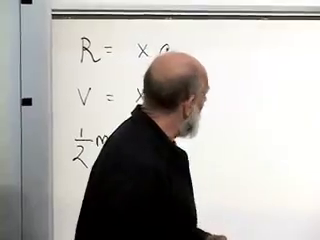
\includegraphics[width=0.72\textwidth]{lecture_09_figure_02.png}
  \caption{La métrique plate en expansion, où le facteur d’échelle multiplie l’élément de ligne spatiale euclidien. Référentiel source à 00:09:12.}
  \label{fig:l09-expanding-metric-board}
\end{figure}

Imaginons des coordonnées peintes sur une feuille de caoutchouc. Les repères de coordonnées restent attachés à la feuille tandis que la distance physique entre eux augmente. Ainsi, une différence de coordonnées telle que « de \(x=0\) à \(x=1\) » n’est qu’une paire de repères. La distance représentée par cet intervalle est \(a(t)\). Trouver l’équation qui régit ce facteur d’échelle est le problème dynamique du cours.

\section{Géométries spatiales fermées, plates et ouvertes}

La platitude est une simplification observationnelle, et non une conséquence de l’homogénéité. Il existe trois géométries spatiales homogènes et isotropes : à courbure positive, nulle et négative. Pour comprendre le cas positif, il est utile de préciser la dimension.

Le lieu
\begin{equation}
  X_1^2+X_2^2=R^2
\end{equation}
est un cercle, ou une sphère de dimension un \(S^1\). Son intérieur rempli est un disque, également appelé boule de dimension deux. En ajoutant une coordonnée d’immersion, on obtient
\begin{equation}
  X_1^2+X_2^2+X_3^2=R^2,
\end{equation}
la sphère ordinaire de dimension deux \(S^2\). En ajoutant une quatrième coordonnée d’immersion, on obtient
\begin{equation}
  X_1^2+X_2^2+X_3^2+X_4^2=R^2,
  \label{eq:l09-three-sphere}
\end{equation}
une sphère de dimension trois \(S^3\), qui est elle-même un espace à trois dimensions. Nous ne pouvons pas nous représenter son immersion en quatre dimensions, mais sa géométrie intrinsèque n’a pas besoin de cette immersion pour exister.

\begin{figure}[H]
  \centering
  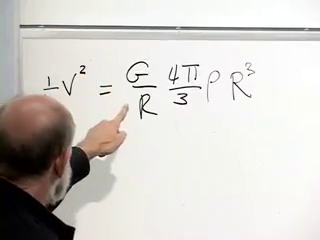
\includegraphics[width=0.72\textwidth]{lecture_09_figure_03.png}
  \caption{L’équation d’immersion utilisée pour introduire la sphère de dimension trois. Référentiel source à 00:16:40.}
  \label{fig:l09-three-sphere-board}
\end{figure}

Tous les points d’une sphère idéale sont géométriquement équivalents, et toutes les directions en un point le sont également. Une sphère est donc à la fois homogène et isotrope. Si son rayon est multiplié par \(a(t)\), tout l’espace se dilate ou se contracte sans qu’un centre soit privilégié sur la sphère. Remonter le cours du temps dans un tel univers ne ramène pas toute la matière à un lieu particulier dans un vide extérieur. L’espace entier devient petit, si bien que chaque paire de points se rapproche. Le Big Bang n’est pas une explosion à partir d’un point de l’espace.

Sur une sphère à courbure positive, la somme des angles d’un triangle géodésique est supérieure à \(180^\circ\). Dans un triangle plat, elle vaut exactement \(180^\circ\). Dans une géométrie homogène à courbure négative, imparfaitement représentée par une selle, elle est inférieure à \(180^\circ\). Ces tests intrinsèques distinguent les trois cas.

\begin{figure}[H]
  \centering
  \includegraphics[width=0.72\textwidth]{lecture_09_figure_07.png}
  \caption{Courbures positive, nulle et négative, représentées par les formes caractéristiques de leurs triangles. Référentiel source à 00:37:30.}
  \label{fig:l09-curvature-board}
\end{figure}

Une métrique parfaitement plate localement ne prouve pas à elle seule que l’espace est topologiquement infini. Des topologies plates compactes sont mathématiquement possibles, même si le cours adopte le modèle euclidien infini le plus simple.
\editorialnote{Cette réserve sur la topologie globale n’est nécessaire pour aucune des dynamiques locales qui suivent.}

\section{Repères comobiles et loi de Hubble}

Revenons à la feuille plate en expansion et traçons-y un quadrillage de coordonnées. En coordonnées comobiles, la grille se dilate avec le flux de matière à grande échelle. Une galaxie, ou plus précisément un amas de galaxies défini à une échelle suffisamment grossière, conserve un repère de coordonnées approximativement fixe, même si sa distance physique à un autre objet comobile varie.

\begin{figure}[H]
  \centering
  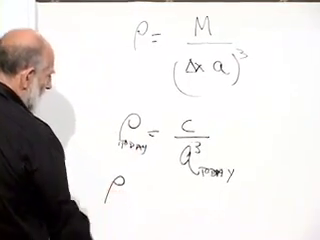
\includegraphics[width=0.72\textwidth]{lecture_09_figure_04.png}
  \caption{Un quadrillage de coordonnées entraîné par une feuille spatiale en expansion. Référentiel source à 00:22:20.}
  \label{fig:l09-comoving-grid-board}
\end{figure}

Pour deux objets séparés le long de l’axe \(x\) par un intervalle comobile fixe \(\Delta x\), leur distance physique est
\begin{equation}
  D(t)=a(t)\,\Delta x.
  \label{eq:l09-physical-distance}
\end{equation}
En dérivant par rapport au temps à \(\Delta x\) constant, on obtient
\begin{equation}
  v(t)=\dot a(t)\,\Delta x
      =\frac{\dot a(t)}{a(t)}D(t).
\end{equation}
En définissant
\begin{equation}
  H(t)\equiv\frac{\dot a(t)}{a(t)},
  \label{eq:l09-hubble-parameter}
\end{equation}
on obtient la loi de Hubble,
\begin{equation}
  v=H(t)D.
  \label{eq:l09-hubble-law}
\end{equation}
Dans l’expression « constante de Hubble », le mot « constante » signifie qu’elle est la même dans tout l’espace à un instant cosmique donné. Cela ne signifie pas qu’elle reste constante au cours de l’histoire cosmique.

\begin{figure}[H]
  \centering
  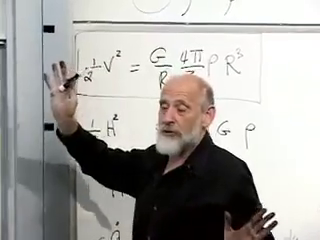
\includegraphics[width=0.72\textwidth]{lecture_09_figure_05.png}
  \caption{La dérivation au tableau \(D=a\Delta x\),
  \(v=(\dot a/a)D=HD\). Référentiel source à 00:26:40.}
  \label{fig:l09-hubble-board}
\end{figure}

\begin{classroomqa}
\audiencequestion{Si l’on observe une galaxie lointaine à une époque antérieure, son paramètre de Hubble inféré devrait-il vraiment être égal à la valeur mesurée aujourd’hui dans notre voisinage ?}
\lecturerresponse{Seulement si le temps rétrospectif est faible devant l’âge de l’Univers. Sur des distances modérées, \(H(t)\) varie assez peu pour qu’une seule valeur soit utile. À des distances véritablement cosmologiques, nous observons des époques plus anciennes, et il faut tenir compte de la dépendance temporelle de \(a\) et de \(H\). C’est l’une des raisons pour lesquelles nous avons besoin d’une équation dynamique pour le facteur d’échelle.}
\end{classroomqa}

\section{Rayons lumineux nuls dans un système de coordonnées en expansion}

\begin{classroomqa}
\audiencequestion{Le facteur d’échelle affecte-t-il la propagation de la lumière entre des galaxies lointaines ?}
\lecturerresponse{Un rayon lumineux suit une trajectoire nulle, donc \(d\tau=0\). Pour un rayon se propageant le long de l’axe positif \(x\), on a \(dy=dz=0\), et la métrique en expansion donne
\begin{align}
  0&=dt^2-a^2(t)dx^2,
  &dt&=a(t)dx,\notag\\
  &&\frac{dx}{dt}&=\frac{1}{a(t)}.
  \label{eq:l09-null-ray}
\end{align}
La vitesse coordonnée diminue à mesure que \(a(t)\) augmente, mais la vitesse physique locale de la lumière reste égale à \(c=1\). Un intervalle de coordonnées fixe représente une distance physique croissante.}
\end{classroomqa}

\begin{figure}[H]
  \centering
  \includegraphics[width=0.72\textwidth]{lecture_09_figure_06.png}
  \caption{La condition de nullité et \(dt=a(t)dx\) pour la propagation radiale de la lumière. Référentiel source à 00:30:54.}
  \label{fig:l09-null-board}
\end{figure}

On pourrait choisir des coordonnées dans lesquelles ce même fait se formulerait ainsi : « la lumière ralentit à mesure qu’on s’éloigne », mais les longueurs et les horloges prendraient alors des descriptions tout aussi peu commodes. Le langage de l’espace en expansion est plus clair, car il préserve l’énoncé local selon lequel tout observateur en chute libre mesure la même vitesse de la lumière.

\begin{classroomqa}
\audiencequestion{Existe-t-il des indices montrant que la propagation locale de la lumière et la physique atomique sont les mêmes dans les galaxies lointaines ?}
\lecturerresponse{Seules les comparaisons sans dimension ont un sens opérationnel. Prenons la taille d’un atome comme unité de longueur et une période atomique ou nucléaire comme unité de temps, puis demandons combien de telles périodes la lumière met à parcourir la longueur choisie. Les observations spectrales étayent l’affirmation selon laquelle ces rapports sans dimension sont les mêmes dans des régions lointaines. Les indices sont indirects, mais c’est précisément par ce type de comparaison que l’on vérifie l’uniformité des lois locales.}
\end{classroomqa}

Lorsque l’Univers observable était extrêmement petit, la lumière pouvait traverser rapidement une région physique donnée, si l’on mesure le temps en temps de traversée de la lumière correspondant à cette région. Cela ne signifie pas que \(c\) était différent. Cela signifie que la région elle-même était petite.

\section{Une sphère newtonienne dans l’Univers}

Passons maintenant de la cinématique à la dynamique. Plaçons-nous à l’origine et traçons une sphère assez grande pour contenir de nombreuses galaxies et de nombreux amas. Choisissons une galaxie sur sa frontière. Dans un univers homogène, la distribution de masse est sphériquement symétrique autour de nous, et le théorème des coquilles de Newton donne deux résultats essentiels :
\begin{enumerate}
  \item toute la matière distribuée sphériquement à l’extérieur du rayon choisi exerce une force newtonienne nette nulle sur la galaxie située à la frontière ;
  \item toute la matière contenue dans la sphère agit, pour ce mouvement radial, comme si elle était concentrée au centre.
\end{enumerate}
Nous choisissons un référentiel dans lequel nous sommes au repos ; les vitesses et les accélérations de l’argument qui suit sont donc mesurées par rapport à nous.

\begin{figure}[H]
  \centering
  \includegraphics[width=0.72\textwidth]{lecture_09_figure_08.png}
  \caption{La construction fondée sur le théorème des coquilles : nous sommes au centre et une galaxie test se trouve sur la frontière d’une grande sphère homogène. Référentiel source à 00:41:10.}
  \label{fig:l09-shell-board}
\end{figure}

\begin{figure}[H]
  \centering
  \begin{tikzpicture}[scale=0.92,>=Latex]
    \draw[thick] (0,0) circle (2.35);
    \fill (0,0) circle (2pt) node[below left] {us};
    \fill (2.35,0) circle (2.2pt) node[right] {test galaxy \(m\)};
    \draw[->,thick,blue!65!black] (0.18,0) -- (2.15,0)
      node[midway,above] {\(R=a(t)x\)};
    \draw[->,thick,red!65!black] (2.35,0.12) -- (3.25,0.12)
      node[midway,above] {\(v=\dot a(t)x\)};
    \node[align=center,text width=7cm] at (0,-2.85)
      {outside shells cancel;\\enclosed mass acts at the center};
  \end{tikzpicture}
  \caption{Reconstitution propre de la construction newtonienne.}
  \label{fig:l09-shell-clean}
\end{figure}

Si la galaxie a pour coordonnée comobile fixe \(x\), son rayon physique et sa vitesse sont
\begin{equation}
  R(t)=x a(t),
  \qquad
  v(t)=x\dot a(t)=H(t)R(t).
  \label{eq:l09-radius-velocity}
\end{equation}
Soit \(M\) la masse contenue dans la sphère et \(m\) la masse de la galaxie test. L’énergie newtonienne est
\begin{equation}
  E=\frac12 m v^2-\frac{GMm}{R}.
  \label{eq:l09-newtonian-energy}
\end{equation}

\begin{figure}[H]
  \centering
  \includegraphics[width=0.72\textwidth]{lecture_09_figure_09.png}
  \caption{La séquence complète au tableau \(R=xa\), \(v=x\dot a\), ainsi que l’équation de l’énergie newtonienne dans le cas particulier \(E=0\). Référentiel source à 00:48:40.}
  \label{fig:l09-energy-board}
\end{figure}

L’énergie peut être positive, nulle ou négative. Commençons à la frontière entre échappement et recollapse, \(E=0\), pour laquelle
\begin{equation}
  \frac12 v^2=\frac{GM}{R}.
  \label{eq:l09-zero-energy}
\end{equation}

\begin{classroomqa}
\audiencequestion{Que signifie une énergie totale nulle pour la galaxie qui s’éloigne ?}
\lecturerresponse{C’est exactement le cas de la vitesse de libération. Une énergie positive correspond à une vitesse supérieure à la vitesse de libération ; une énergie négative, à une vitesse inférieure, et, dans le cadre newtonien où seule la matière intervient, à un retour éventuel. Nous commençons à la frontière entre ces possibilités et reviendrons aux autres signes après avoir dérivé l’équation du cas plat.}
\end{classroomqa}

\begin{classroomqa}
\audiencequestion{La masse contenue \(M\) varie-t-elle à mesure que la sphère s’étend ?}
\lecturerresponse{Non. La sphère est comobile, de sorte que les mêmes particules restent à l’intérieur. Son volume physique augmente et sa densité diminue, mais sa masse totale contenue reste constante. Cette distinction entre \(M\) et \(\rho(t)\) est essentielle.}
\end{classroomqa}

Pour une densité homogène \(\rho(t)\),
\begin{equation}
  M=\frac{4\pi}{3}\rho(t)R^3.
  \label{eq:l09-enclosed-mass}
\end{equation}
La substitution dans \eqref{eq:l09-zero-energy} donne
\begin{equation}
  \frac12 v^2
  =\frac{G}{R}\left(\frac{4\pi}{3}\rho R^3\right).
  \label{eq:l09-enclosed-energy}
\end{equation}

\begin{figure}[H]
  \centering
  \includegraphics[width=0.72\textwidth]{lecture_09_figure_10.png}
  \caption{La substitution de la masse contenue dans l’équation à énergie nulle. Référentiel source à 00:54:16.060.}
  \label{fig:l09-enclosed-mass-board}
\end{figure}

En utilisant \(v=HR\), on trouve
\begin{align}
  \frac12 H^2R^2
    &=\frac{4\pi G}{3}\rho R^2,\\
  H^2
    &=\frac{8\pi G}{3}\rho.
\end{align}
La loi d’expansion plate à énergie nulle est donc
\begin{equation}
  \boxed{\left(\frac{\dot a}{a}\right)^2
  =\frac{8\pi G}{3}\rho(t)}.
  \label{eq:l09-flat-friedmann}
\end{equation}
L’élimination de \(R^2\) n’est pas fortuite. Dans un univers homogène, \(H(t)\) doit être le même quel que soit l’objet comobile choisi comme objet test.

\begin{figure}[H]
  \centering
  \includegraphics[width=0.72\textwidth]{lecture_09_figure_11.png}
  \caption{L’élimination du rayon et la relation de Friedmann qui en résulte au tableau pour le cas plat. Référentiel source à 00:57:30.}
  \label{fig:l09-friedmann-board}
\end{figure}

\begin{classroomqa}
\audiencequestion{Existe-t-il des indices en faveur de la relation à énergie nulle ?}
\lecturerresponse{On peut inférer les deux membres de la relation à partir des observations : \(H\) à partir des données sur la récession et \(\rho\) en tenant compte des étoiles, du gaz, de la matière noire et de l’énergie du vide. La comparaison à l’époque du cours trouvait les deux membres compatibles à environ un pour cent près. Cette réserve est importante : il faut inclure toutes les formes d’énergie, et la discussion ultérieure de l’énergie du vide modifie l’interprétation naïve en termes de vitesse de libération.}
\end{classroomqa}

Dans les unités \(c=1\), la densité de masse et la densité d’énergie ont les mêmes unités. Le symbole \(\rho\) désignera donc la densité d’énergie totale pertinente pour le composant considéré.

\section{La matière ordinaire et la loi en deux tiers}

L’équation \eqref{eq:l09-flat-friedmann} ne forme pas un système fermé tant que nous ne savons pas comment \(\rho(t)\) varie. Remplissons d’abord une boîte rectangulaire comobile de particules lentes et non relativistes. Ses dimensions en coordonnées restent fixes, tandis que son volume physique augmente comme
\begin{equation}
  V(t)=a^3(t)\,\Delta x\,\Delta y\,\Delta z.
\end{equation}
Le nombre de particules et leur masse au repos dans la boîte restent fixes, donc
\begin{equation}
  \rho_{\mathrm m}(t)=\frac{C_{\mathrm m}}{a^3(t)}.
  \label{eq:l09-matter-dilution}
\end{equation}
En normalisant à l’époque actuelle \(t_0\),
\begin{equation}
  \frac{\rho_{\mathrm m}(t)}{\rho_{\mathrm m,0}}
  =\left(\frac{a_0}{a(t)}\right)^3.
  \label{eq:l09-matter-normalized}
\end{equation}

\begin{figure}[H]
  \centering
  \includegraphics[width=0.72\textwidth]{lecture_09_figure_12.png}
  \caption{La densité de matière, sa dilution en \(a^{-3}\) et la normalisation à l’époque actuelle. Référentiel source à 01:04:47.940.}
  \label{fig:l09-density-board}
\end{figure}

\begin{classroomqa}
\audiencequestion{Quelle est l’ordre de grandeur de la densité d’énergie actuelle de l’Univers, et les atomes ordinaires peuvent-ils à eux seuls la fournir ?}
\lecturerresponse{Un décompte de la matière baryonique visible ne donne qu’une partie de la réponse. Il faut aussi représenter la matière noire et l’énergie noire comme des équivalents masse-énergie. Le cours cite un ordre de grandeur allant d’un atome à quelques dizaines d’équivalents de masse de l’hydrogène par mètre cube, en soulignant qu’il s’agit d’un ordre de grandeur et non d’un inventaire précis.}
\end{classroomqa}

Introduisons \eqref{eq:l09-matter-dilution} dans \eqref{eq:l09-flat-friedmann} et regroupons tous les facteurs indépendants du temps dans une constante positive \(C\) :
\begin{equation}
  \left(\frac{\dot a}{a}\right)^2=\frac{C}{a^3},
  \qquad
  \dot a^2=\frac{C}{a}.
  \label{eq:l09-matter-ode}
\end{equation}
Deux méthodes simples permettent de la résoudre. Une solution d’essai en loi de puissance \(a=K t^p\) impose
\begin{equation}
  p-1=-\frac{p}{2},
  \qquad p=\frac23.
\end{equation}
On peut aussi prendre la branche de la racine carrée correspondant à l’expansion et intégrer :
\begin{equation}
  a^{1/2}\frac{da}{dt}=\sqrt C,
  \qquad
  \int a^{1/2}da=\sqrt C\int dt,
\end{equation}
Ainsi, en choisissant l’origine des temps au Big Bang,
\begin{equation}
  a^{3/2}\propto t,
  \qquad
  \boxed{a(t)\propto t^{2/3}}.
  \label{eq:l09-matter-solution}
\end{equation}
Pendant la dérivation en direct, un facteur est brièvement perdu lors de l’identification des coefficients ; l’intégrale est ensuite reprise pour vérifier l’exposant. Les notes conservent cette vérification, mais ne présentent que l’algèbre corrigée.

\begin{figure}[H]
  \centering
  \includegraphics[width=0.72\textwidth]{lecture_09_figure_13.png}
  \caption{La solution d’essai en loi de puissance et l’exposant encadré \(p=2/3\). Référentiel source à 01:13:05.}
  \label{fig:l09-matter-solution-board}
\end{figure}

La dérivation de la solution donne
\begin{equation}
  H(t)=\frac{\dot a}{a}=\frac{2}{3t}.
  \label{eq:l09-matter-hubble}
\end{equation}
Le paramètre de Hubble était plus grand dans le passé. Par conséquent, quand on regarde assez loin pour que le temps rétrospectif soit appréciable, il ne faut pas prolonger la relation linéaire locale en utilisant sans modification le \(H_0\) d’aujourd’hui.

\begin{figure}[H]
  \centering
  \includegraphics[width=0.72\textwidth]{lecture_09_figure_14.png}
  \caption{En prenant \(\dot a/a\) pour \(a\propto t^{2/3}\), on obtient
  \(H=2/(3t)\). Référentiel source à 01:20:42.}
  \label{fig:l09-hubble-time-board}
\end{figure}

\section{Signe de l’énergie et courbure spatiale}

Le raisonnement newtonien nous a menés jusqu’au cas plat à énergie nulle. La relativité générale ajoute un fait que le seul théorème des coquilles ne permet pas d’obtenir : le signe de l’énergie spécifique de type newtonien correspond au signe de la courbure spatiale.
\begin{center}
\begin{tabular}{@{}>{\raggedright\arraybackslash}p{0.20\linewidth}
                    >{\raggedright\arraybackslash}p{0.29\linewidth}
                    >{\raggedright\arraybackslash}p{0.37\linewidth}@{}}
  \toprule
  Énergie totale & Courbure spatiale & Évolution avec la matière seule \\
  \midrule
  positive & négative (ouverte) & expansion éternelle \\
  nulle & nulle (plate) & tend vers la limite d’échappement \\
  négative & positive (fermée) & expansion, retournement, recollapse \\
  \bottomrule
\end{tabular}
\end{center}
La dernière colonne suppose l’absence d’énergie du vide. Dans l’analogie du projectile, une énergie positive correspond à une vitesse supérieure à la vitesse de libération, une énergie nulle à une vitesse exactement égale à celle-ci, et une énergie négative à une vitesse inférieure. Les équations d’Einstein associent respectivement ces trois cas aux géométries spatiales ouverte, plate et fermée.

\section{Photons et loi en un demi}

La loi de la matière \(\rho\propto a^{-3}\) suppose que l’énergie de chaque particule est approximativement constante tandis que la densité numérique diminue. Les photons ne satisfont pas cette hypothèse. Pour un photon,
\begin{equation}
  E=h\nu=\frac{hc}{\lambda}.
\end{equation}
L’expansion étire sa longueur d’onde proportionnellement au facteur d’échelle,
\begin{equation}
  \lambda\propto a,
  \qquad E\propto a^{-1}.
\end{equation}
La densité numérique de photons diminue toujours comme \(a^{-3}\), et l’énergie de chaque photon apporte un facteur supplémentaire \(a^{-1}\). Par conséquent,
\begin{equation}
  \boxed{\rho_{\mathrm r}(t)\propto a^{-4}(t)}.
  \label{eq:l09-radiation-dilution}
\end{equation}

L’analogie avec une corde de guitare rend l’image physique intuitive. On pince une corde, puis on allonge la partie qui vibre : la longueur d’onde augmente et le son devient plus grave. Un mode photonique dans une boîte comobile en expansion se comporte de façon analogue. En remontant le cours du temps, la compression raccourcit les longueurs d’onde et augmente l’énergie des photons.

\begin{figure}[H]
  \centering
  \includegraphics[width=0.72\textwidth]{lecture_09_figure_15.png}
  \caption{La relation pour la densité de matière prolongée au tableau jusqu’à la loi d’échelle du rayonnement \(\rho_{\mathrm r}\propto a^{-4}\). Référentiel source à 01:29:20.}
  \label{fig:l09-radiation-board}
\end{figure}

En utilisant \(\rho_{\mathrm r}\propto a^{-4}\) dans l’équation de Friedmann pour le cas plat, on obtient
\begin{equation}
  \left(\frac{\dot a}{a}\right)^2=\frac{C_{\mathrm r}}{a^4},
  \qquad
  \dot a\propto a^{-1},
\end{equation}
puis
\begin{equation}
  \boxed{a(t)\propto t^{1/2}}.
  \label{eq:l09-radiation-solution}
\end{equation}
Cette croissance est plus lente que \(t^{2/3}\). Assez loin dans le passé, le rayonnement doit dominer la matière ordinaire, car \(a^{-4}\) augmente plus vite que \(a^{-3}\) à mesure que \(a\) diminue. Le cours situe le passage entre les dominations du rayonnement et de la matière à l’époque où le facteur d’échelle était environ mille fois plus petit qu’aujourd’hui. Avant ce passage, l’Univers était dominé par le rayonnement ; après, il a été dominé par la matière pendant une longue période.

\section{Énergie du vide et expansion exponentielle}

L’énergie du vide suit une loi d’échelle opposée. Sa densité est une propriété de l’espace vide et ne se dilue pas avec l’expansion de l’Univers :
\begin{equation}
  \rho_\Lambda=\text{constant}.
  \label{eq:l09-vacuum-density}
\end{equation}
La matière ordinaire et le rayonnement deviennent plus denses quand on remonte vers le passé, tandis que ce terme ne varie pas. Il était donc moins important dans l’Univers primordial et devient plus important à mesure que les autres composantes se diluent. Le cours reprend l’estimation alors en vigueur, selon laquelle l’énergie du vide fournit environ \(70\%\) de la densité d’énergie cosmique actuelle.

Pour \(\rho_\Lambda\) constant, l’équation \eqref{eq:l09-flat-friedmann} donne un taux d’expansion constant
\begin{equation}
  H_\Lambda=\sqrt{\frac{8\pi G}{3}\rho_\Lambda},
  \qquad
  \frac{\dot a}{a}=H_\Lambda.
\end{equation}
Par conséquent,
\begin{equation}
  \boxed{a(t)=a(t_i)e^{H_\Lambda(t-t_i)}}.
  \label{eq:l09-vacuum-solution}
\end{equation}

\begin{figure}[H]
  \centering
  \includegraphics[width=0.72\textwidth]{lecture_09_figure_16.png}
  \caption{L’équation à densité constante qui conduit à l’expansion exponentielle. Référentiel source à 01:35:48.}
  \label{fig:l09-vacuum-board}
\end{figure}

À l’échelle observée citée dans le cours, l’Univers double de taille linéaire en environ dix à douze milliards d’années. L’origine de cette faible densité du vide, mais non nulle, reste inexpliquée ; son existence et son effet sur l’expansion sont des faits empiriques.

\begin{classroomqa}
\audiencequestion{L’énergie du vide désigne-t-elle la même chose que l’énergie noire dans cette discussion ?}
\lecturerresponse{Oui. Ici, « énergie noire » désigne une densité constante d’énergie du vide, équivalente à une constante cosmologique. On peut imaginer des modèles plus généraux d’énergie noire dépendant du temps, mais ils ne font pas partie du calcul présenté dans ce cours.}
\end{classroomqa}

\section{Comment l’expansion de l’Univers décale la lumière vers le rouge}

\begin{classroomqa}
\audiencequestion{Comment les photons peuvent-ils savoir que nous avons choisi des coordonnées comobiles en expansion et donc qu’ils doivent perdre de l’énergie ?}
\lecturerresponse{Ils ne réagissent pas à nos repères. Ils se propagent dans une géométrie où les distances physiques varient. Un train d’ondes occupant une région dont la taille physique double voit sa longueur d’onde doubler. Les coordonnées comobiles ne font que décrire efficacement cet étirement ; elles ne le provoquent pas.}
\end{classroomqa}

\begin{classroomqa}
\audiencequestion{D’où viennent les photons du rayonnement de fond qui nous parviennent aujourd’hui ?}
\lecturerresponse{Regarder plus loin, c’est regarder plus tôt. Nous finissons par observer l’époque où la matière cosmique était un plasma ionisé, opaque parce que les photons étaient diffusés à répétition par des particules chargées libres. La frontière d’où les photons ont pu voyager librement jusqu’à nous apparaît comme une sphère entourant l’observateur : la surface de dernière diffusion.}
\end{classroomqa}

\begin{figure}[H]
  \centering
  \includegraphics[width=0.72\textwidth]{lecture_09_figure_17.png}
  \caption{Schéma centré sur l’observateur, montrant la surface de dernière diffusion et des coquilles de plus en plus éloignées. Référentiel source à 01:42:05.}
  \label{fig:l09-last-scattering-board}
\end{figure}

\begin{figure}[H]
  \centering
  \begin{tikzpicture}[scale=0.9,>=Latex]
    \fill (0,0) circle (2pt) node[below] {observer};
    \draw[thick,orange!70!black] (0,0) circle (2.55);
    \node[orange!70!black,align=center] at (0,3.05)
      {surface of last scattering};
    \foreach \a in {25,75,145,210,285,335}{
      \draw[->,blue!60!black] ({2.55*cos(\a)},{2.55*sin(\a)}) --
        ({1.7*cos(\a)},{1.7*sin(\a)});
    }
    \draw[decorate,decoration={snake,amplitude=1.5pt,segment length=7pt},
      red!65!black,thick,->] (-2.5,0) -- (-0.15,0);
    \node[red!65!black,below] at (-1.35,-0.15)
      {redshifted photon};
  \end{tikzpicture}
  \caption{Reconstitution propre de la représentation de la dernière diffusion.}
  \label{fig:l09-last-scattering-clean}
\end{figure}

Le rayonnement a été émis avec un spectre caractéristique d’un plasma chaud et nous parvient avec des longueurs d’onde environ mille fois plus grandes. Dans le vocabulaire Doppler du cours, la surface émettrice lointaine s’éloigne rapidement et son rayonnement est fortement décalé vers le rouge. Dans la description géométrique, l’onde s’étire au cours de sa propagation. Les deux représentations expriment la même relation,
\begin{equation}
  1+z=\frac{\lambda_0}{\lambda_{\mathrm{em}}}
      =\frac{a_0}{a_{\mathrm{em}}}.
  \label{eq:l09-cosmological-redshift}
\end{equation}
\editorialnote{L’équation \eqref{eq:l09-cosmological-redshift} donne la forme quantitative usuelle des descriptions de l’étirement et de l’effet Doppler présentées dans le cours.}

À une époque d’observation antérieure, la sphère de dernière diffusion aurait été plus proche dans la représentation correspondante, et les photons du rayonnement de fond observés auraient été moins décalés vers le rouge et donc plus énergétiques. Au fil du temps cosmique, les photons qui parviennent à un observateur comobile depuis ce plasma primordial ont des longueurs d’onde de plus en plus grandes.

\section{Où va l’énergie d’un photon décalé vers le rouge ?}

\begin{classroomqa}
\audiencequestion{Un photon est émis avec une énergie \(h\nu_{\mathrm{em}}\) et arrive, décalé vers le rouge, avec une énergie plus faible. Qu’est-il advenu de la différence ?}
\lecturerresponse{La dérivation newtonienne commençait par une équation d’énergie. Sa forme cosmologique relie le taux d’expansion à la densité d’énergie de la matière ; l’énergie de la matière et l’expansion ne peuvent donc pas être considérées comme des bilans conservés séparément. Le cours décrit l’énergie perdue par les photons comme entrant dans le bilan cinétique de l’expansion. Un piston rempli de rayonnement concrétise l’analogie : la pression du rayonnement pousse le piston vers l’extérieur, les longueurs d’onde des photons augmentent et leur énergie perdue devient le travail mécanique et l’énergie cinétique du piston.}
\end{classroomqa}

\begin{figure}[H]
  \centering
  \includegraphics[width=0.72\textwidth]{lecture_09_figure_18.png}
  \caption{Le tableau place l’équation d’énergie newtonienne encadrée au-dessus de l’équation de Friedmann correspondante. Référentiel source à 01:44:42.}
  \label{fig:l09-energy-bookkeeping-board}
\end{figure}

\begin{classroomqa}
\audiencequestion{Qu’est-ce qui couple l’énergie du rayonnement à l’expansion ?}
\lecturerresponse{La pression. Dans un cylindre muni d’un piston mobile, les photons transmettent leur quantité de mouvement à la paroi. Lorsque le piston se déplace, le rayonnement fournit un travail ; sa longueur d’onde augmente et son énergie diminue. L’Univers homogène en expansion n’a pas de piston extérieur au sens littéral, mais l’analogie \(p\,dV\) explique pourquoi la densité d’énergie du rayonnement diminue plus vite que ne le ferait la seule dilution numérique.}
\end{classroomqa}

\begin{figure}[H]
  \centering
  \includegraphics[width=0.72\textwidth]{lecture_09_figure_19.png}
  \caption{Le piston mobile rempli de photons, utilisé pour illustrer le travail de la pression. Référentiel source à 01:46:40.}
  \label{fig:l09-piston-board}
\end{figure}

\begin{figure}[H]
  \centering
  \begin{tikzpicture}[scale=0.92,>=Latex]
    \draw[thick] (0,0) rectangle (5.3,2.6);
    \draw[very thick] (4.25,0) -- (4.25,2.6);
    \draw[very thick] (4.25,1.3) -- (5.25,1.3);
    \draw[->,thick,red!65!black] (5.25,1.3) -- (6.2,1.3)
      node[right] {moving piston};
    \foreach \y in {0.55,1.3,2.05}{
      \draw[decorate,decoration={snake,amplitude=1.4pt,segment length=6pt},
        blue!65!black,->] (0.35,\y) -- (3.9,\y);
    }
    \node at (2.15,-0.45) {radiation does \(p\,dV\) work};
  \end{tikzpicture}
  \caption{Reconstitution propre de l’analogie du piston rempli de rayonnement.}
  \label{fig:l09-piston-clean}
\end{figure}

L’énergie en relativité générale demande quelques précautions. Dans un espace-temps en expansion quelconque, il n’existe pas nécessairement d’énergie globale conservée unique, analogue à l’énergie d’un système newtonien isolé. La conservation locale du tenseur énergie-impulsion reste valable et, pour un fluide homogène, elle conduit à l’équation de continuité
\begin{equation}
  \dot\rho+3H(\rho+p)=0,
  \label{eq:l09-continuity}
\end{equation}
qui contient le terme de travail de pression à l’origine des lois d’évolution de la matière et du rayonnement.\editorialnote{L’équation \eqref{eq:l09-continuity} est l’énoncé local précis de la relativité générale qui sous-tend l’analogie, délibérément newtonienne, entre l’énergie cosmologique et un bilan comptable.}

L’énergie du vide rend le problème particulièrement aigu. Sa densité restant constante tandis que le volume augmente, l’énergie totale du vide dans une région comobile croît. Sa pression négative contribue à la source gravitationnelle et provoque une expansion accélérée. Il ne faut donc pas exiger la conservation séparée de la naïve « énergie de la matière dans une boîte comobile » sans tenir compte de la géométrie et du travail de pression.

\section{Pourquoi peut-on éliminer le facteur d’échelle du terme temporel}

\begin{classroomqa}
\audiencequestion{Pourquoi le facteur d’échelle multiplie-t-il la partie spatiale de la métrique, mais pas sa partie temporelle ?}
\lecturerresponse{C’est un choix de coordonnée temporelle. Supposons que l’on parte d’une coordonnée de temps conforme \(t\), avec
\begin{equation}
  d\tau^2=A^2(t)\left(dt^2-dx^2\right).
\end{equation}
Définissons un nouveau temps cosmique \(T\) par
\begin{equation}
  dT=A(t)\,dt.
\end{equation}
On obtient alors
\begin{equation}
  d\tau^2=dT^2-A^2\bigl(t(T)\bigr)dx^2.
\end{equation}
Le facteur commun qui multipliait le différentiel temporel a disparu, tandis que le facteur d’échelle physique demeure dans le terme spatial.}
\end{classroomqa}

\begin{figure}[H]
  \centering
  \includegraphics[width=0.72\textwidth]{lecture_09_figure_20.png}
  \caption{La redéfinition du temps \(dT=A(t)dt\) qui transforme le temps conforme en temps cosmique. Image source à 01:51:05.}
  \label{fig:l09-time-reparam-board}
\end{figure}

\section{Courbure, énergie du vide et destin cosmique}

\begin{classroomqa}
\audiencequestion{Si l’Univers était positivement courbé, devrait-on déjà voir des galaxies venir vers nous ?}
\lecturerresponse{Pas nécessairement. Un projectile lancé à une vitesse inférieure à la vitesse de libération se déplace d’abord vers l’extérieur, atteint un point de rebroussement, puis seulement retombe. Nous observons l’Univers pendant une phase d’expansion. En l’absence d’énergie du vide, un univers de matière à courbure positive finirait par s’effondrer à nouveau. Une énergie du vide positive suffisamment grande empêche ce retournement, et sa valeur observée semble assez élevée pour entraîner une expansion exponentielle à long terme, même si la courbure spatiale est faible.}
\end{classroomqa}

L’avenir exponentiel n’est pas un paradis énergétique. Les étoiles finissent par s’éteindre, les densités de matière et de rayonnement diminuent de façon exponentielle et les régions lointaines sortent du contact causal. L’énergie du vide persiste tandis que les structures ordinaires deviennent progressivement plus froides et plus diffuses.

\begin{classroomqa}
\audiencequestion{En remontant plus loin dans le passé, y avait-il davantage de photons que de particules ordinaires ?}
\lecturerresponse{Le rapport entre le nombre de photons et celui des baryons est déjà immense : selon l’estimation du cours, il y a environ \(10^{10}\) photons par baryon, et ces deux nombres restent approximativement constants dans un volume comobile. En remontant vers le passé, c’est principalement l’énergie de chaque photon qui change. L’énergie des photons augmente comme \(a^{-1}\), tandis que les masses au repos non relativistes, elles, ne changent pas. Le rayonnement domine donc la densité d’énergie aux premiers instants, même si le rapport entre les nombres de particules n’a pas besoin de changer.}
\end{classroomqa}

La leçon essentielle est que la géométrie, à elle seule, ne détermine pas l’histoire cosmique. L’équation de Friedmann pour un univers plat établit la relation entre l’expansion et la densité d’énergie, mais c’est le contenu matériel qui en détermine l’évolution temporelle. La matière non relativiste donne \(a\propto t^{2/3}\), le rayonnement donne \(a\propto t^{1/2}\) et une énergie du vide constante entraîne une expansion exponentielle. Ces trois lois organisent les ères successives de l’Univers et expliquent pourquoi le même facteur d’échelle détermine les distances, les décalages vers le rouge et l’évolution du paramètre de Hubble.

\end{document}